\documentclass{report}

%%%%%%%%%%%%%%%%%%%%%%%%%%%%%%%%%%%%%%%%

\usepackage[utf8]{inputenc}

%%%%%%%%%%%%%%%%%%%%%%%%%%%%%%%%%%%%%%%%

\usepackage{tikz}
\usepackage{pgfplots}
\pgfplotsset{compat=1.5}

\usetikzlibrary{external}
\tikzexternalize
\tikzsetexternalprefix{tikzexternal/}

%%%%%%%%%%%%%%%%%%%%%%%%%%%%%%%%%%%%%%%%

\usepackage{amsmath,amsfonts,amssymb}
\renewcommand{\baselinestretch}{1.0}
\usepackage{graphicx}
\usepackage[colorlinks=true, allcolors=blue]{hyperref}
\definecolor{gray}{gray}{0.75}
\definecolor{ligray}{gray}{0.9}
\usepackage{lscape}
\usepackage{enumitem}

\usepackage{chngcntr}
\counterwithin{figure}{section}
\counterwithin{table}{section}

%%%%%%%%%%%%%%%%%%%%%%%%%%%%%%%%%%%%%%%%

\setlength{\parindent}{0pt}
\setlength{\parskip}{\medskipamount}
\usepackage{setspace}

%%%%%%%%%%%%%%%%%%%%%%%%%%%%%%%%%%%%%%%%

\usepackage{newtxtext,newtxmath}

% Instead of the above, use this for arXiv:

%\usepackage{txfonts}
%\usepackage{textcomp}
%\usepackage{eurosym}
%\let\texteuro\euro

%%%%%%%%%%%%%%%%%%%%%%%%%%%%%%%%%%%%%%%%

\newcommand{\unit}[1]{\ensuremath{\mathrm{#1}}}
\newcommand{\micron}{\mbox{$\mu$m}}
\newcommand{\mm}{\mbox{mm}}
\newcommand{\sqmm}{\mbox{mm$^2$}}
\renewcommand{\deg}{\mbox{deg}}
\newcommand{\sqdeg}{\mbox{$\deg^2$}}
\newcommand{\persqdeg}{\mbox{$\deg^{-2}$}}
\newcommand{\arcmin}{\mbox{arcmin}}
\newcommand{\sqarcmin}{\mbox{\arcmin$^2$}}
\newcommand{\persqarcmin}{\mbox{\arcmin$^{-2}$}}
\newcommand{\arcsec}{\mbox{arcsec}}
\newcommand{\sqarcsec}{\mbox{\arcsec$^2$}}
\newcommand{\persqarcsec}{\mbox{\arcsec$^{-2}$}}
\newcommand{\Hs}{\mbox{$H_\mathrm{s}$}}
\newcommand{\CaF}{\ensuremath{\mathrm{CaF_2}}}

\newcommand{\TODO}[1]{\textcolor{red}{TODO: #1}}

%%%%%%%%%%%%%%%%%%%%%%%%%%%%%%%%%%%%%%%%

\begin{document}

\pagestyle{empty}

\begin{center}
\Large \bfseries
DDRAGO and WOB\\Mechanical Design
\end{center}

\vspace{2cm}

\begin{center}

\begin{center}
\begin{tabular}{ll}
Prepared by:&Rosalía Langarica\\
&Alejandro Farah\\
&Silvio Tinoco\\
&Jaime Ruíz\\
&Jorge Fuentes-Fernández\\
&Salvador Cuevas\\
&Alan M. Watson\\
Reviewed by:&Alan M. Watson\\
&Rosalía Langarica\\
Approved by:&Alan M. Watson\\
&Rosalía Langarica\\
Reference&GFT-MD-A3135-041-UNAM\\
Version:& 3.3\\
Date:&30 March 2022\\
\end{tabular}
\end{center}

\vspace{\fill}

%\begin{center}
DDRAGO Project\\
Instituto de Astronomí­a\\
Universidad Nacional Autónoma de México
\end{center}

\clearpage
\section*{Document Change Record}

\begin{itemize}
\item Version 3.3 of 30 March 2022.

\begin{itemize}
\item Added a section on the counterweights.
\item Added information on the lifting eye-bolts.

\end{itemize}

\item Version 3.2 of 25 January 2022.

Minor updates in preparation for the FDR

\item Version 3.1 of 19 January 2022.

Extensive updates in preparation for the FDR

\item Version 3.0 of 16 April 2021.

\begin{itemize}
\item Update after DDRAGUITO.
\end{itemize}

\item Version 2.0 of 15 September 2017.

{\it Modifications from the previous version}

\begin{itemize}
\item Updated the design and analysis of the support structure.
\item Removed passive ventilation of the support structure.
\item Updated the designs of the lens mounts to use silicone O-rings for thermal compensation.
\item We will use black anodizing type II.
\end{itemize}

{\it New material}
\begin{itemize}
\item Analysis of birefringence in the DDRAGO lenses.
\end{itemize}

\item Version 1.0 of 22 January 2017.

Initial version.
\end{itemize}

\clearpage

\section*{Applicable Documents}

\begin{enumerate}[label={AD\arabic*}]
\item \label{FPRD} Vives, S., and R\'egal, X.,Floriot, J. “Functional and Performance Requirements Documents”, GFT-FPRD-6.6
\item \label{product-tree} Watson, A. M., “DDRAGO Product Tree”
\item \label{optics} Fuentes-Fernández,~J., Watson, A. M., \& Cuevas, S., “COLIBRI Optical Design”, GFT-OD-A3135-040-UNAM-5.1
\item \label{aiv} Cuevas,~S., Fuentes-Fernández,~J., Watson,~A.~M., \& Ángeles,~F., “DDRAGO and CAGIRE WOB AIV Plan”, GFT-OD-A3135-043-UNAM-2.0
\item \label{aivDDRAGUITO} Fuentes-Férnandez,~J., Langarica,~R., Tinoco,~S., Álvarez,~L.~C. \& Cuevas,~S., ``Assembly and Verification of the DDRAGUITO Lens Systems''.
\end{enumerate}

\section*{Reference Documents}

\begin{enumerate}[label={RD\arabic*}]
\item \label{yoder15} Yoder, P. R and Vukobratovich, D., ``Opto-mechanical Systems Design", CRC Press, Fourth Ed., Vol. 1, Section 11.4.3. (2015)

\item \label{karow} Karow, H.H., [Fabrication methods for Precision Optics], Wiley, New York (1993).

\item \label{hopkins} Hopkins, R.E., “Lens Mounting and Centering”, chap. 2, [Applied Optics and Optical Engineering], Vol. VIII, Academic Press, New York (1980).
\item \label{ino} http://www.ino.ca/en/examples/lens-auto-centering-technology/

\item \label{parker} Parker O-Ring Handbook. 2001 Edition. Catalog 5700A/US, Section II, p.27.
Parker Hannifin Corporation, Cleveland, OH.

\item \label{black} Robinson,~F.~D., “RATIR Black Paint”, unpublished technical report, 2010.

\end{enumerate}

\clearpage

\pagestyle{plain}

\tableofcontents
\clearpage

\listoffigures
\clearpage

\listoftables
\clearpage

\chapter{Introduction}

This document describes the mechanical design of the DDRAGO instrument and the CAGIRE instrument WOB (warm optical bench).

\section{DDRAGO and CAGIRE}

DDRAGO is a wide-field, two-channel optical imager, with one blue channel observing in $gri$ and the other red channel in $zy$. Both channels are equipped with $\mathrm{4k} \times \mathrm{4k}$ CCDs covering a field of $26\times26$ arcmin.

The DDRAGO instrument works in conjunction with the CAGIRE infrared imager, which has one channel observing in $JH$. This channel has an ALFA $\mathrm{2k}\times\mathrm{2k}$ detector covering a field of $22\times22$ arcmin centered on the DDRAGO field. DDRAGO provides reimaging to CAGIRE through ambient-temperature optics mounted on the WOB (“warm optical bench”) and supports the CAGIRE cryostat, filter mechanism, and close electronics.

The DDRAGO/CAGIRE combination mounts on one of the Nasmyth ports of the COLIBRÍ 1.3-meter telescope. A derotator will compensate for field rotation, but only through a limited range of $\pm65$ deg, which is enough to allow us to align North with either the detector rows or columns.

\section{DDRAGUITO}

DDRAGUITO is a test instrument for the COLIBRÍ telescope. It consists essentially of the blue channel of DDRAGO unfolded and packages in a simple support structure. It was shipped to LAM in March 2021 and is currently awaiting installation on the telescope.

The relevance of DDRAGUITO to the mechanical design of DDRAGO is that we propose to reuse the OML1L2 optomechanics from DDRAGUITO without modification in DDRAGO. This assemblage holds the large L1 and L2 lenses, and we desire to reuse it since it thoroughly satisfies the optical requirements.

We also propose to reuse the OML3 barrel from DDRAGUITO that hosts the blue channel L3 field lens. Nevertheless, the original lens (L3) will be replaced with a new one since the coatings of the original lens were slightly damaged during the grinding of its bevel.


%DDRAGUITO is a test instrument for the COLIBRÍ telescope. It consists essentially of the blue channel of DDRAGO unfolded and packages in a simple support structure. It was shipped to LAM in March 2021 and is currently awaiting installation on the telescope.

%The relevance of DDRAGUITO to the mechanical design of DDRAGO is that we propose to reuse the OML1L2 barrel from DDRAGUITO without modification in DDRAGO. This barrel holds the large L1 and L2 lenses, and we desire to reuse it since human resources for manufacturing are likely to be limited. We are using it without modification to avoid having to remove the lenses, since the large $\mathrm{CaF_2}$ L1 lens is the most expensive lens in the whole instrument, surpassing even the aspherical L8 lens. As we shall see, this complicates the optomechanics of DDRAGO somewhat. We also propose to reuse the OML3 barrel from DDRAGUITO that hosts the small L3 field lens. 

%The mechanical design is at different levels of maturity. 

%We consider the support structure and the main optomechanics of DDRAGO (the supports for L1 to L4, D1 and D2, the filter wheels, and the detectors) to be almost at the level CDR. These are the most critical items in terms of our schedule for delivering a test camera to OHP early 2019.

%However, we have not worked on the CAGIRE WOB since PDR. Furthermore the interfaces between the support structure and CAGIRE (the cryostat, close electronics, and wiring) and the external wiring of DDRAGO are also immature. We have also not yet propagated the design change seen in the optomechanics for D1 and D2 into those for CP. We expect most of these items will improve before the full CDR in November 2017, but the detailed design of the CAGIRE WOB will likely be delayed to 2018.

\section{Optical Design}

The optical design is described in detail in \ref{optics}. However, for convenience we describe it briefly here with reference to Figures~\ref{figure:optics-layout-3d}, \ref{figure:optics-schematic},  and \ref{figure:optics-layout-2d}, which are taken from \ref{optics}.

The beam from M3 enters the instrument through the doublet L1L2. It then encounters the inclined dichroic D1, which reflects $grizy$ light towards the blue and red channels and transmits $JH$ light to the infrared channel.

The $grizy$ light reflected by D1 then encounters a second inclined dichroic D2 (inclined at 90 degrees to D1), which reflects the $gri$ light into the blue channel and transmits the $zy$ light into the red channel. In both channels, the light then encounters a field lens (L3 in the blue channel and L4 in the red channel), a filter wheel, and finally the detector. The astigmatism introduced by transmission through D1 is compensated by a wedge in D2 and by a tilt in L4.

The $JH$ light transmitted by D1 subsequently encounters the inclined corrector plate CP. The astigmatism introduced by transmission through D1 is compensated by a wedge in D1 and by CP. The beam is then folded by fold mirrors FM1, FM2, and FM3 through the WOB optics and into the cryostat. The powered WOB optics consists of three singlets L5, L6, and L7 and a quadruplet L8L9L10L11 (which is formally a cemented doublet L8L9 and two singles L10 and L11, but we mount them in one barrel as if they were a quadruplet). After L11, the beam passes through the filter and then the cryostat window. Within the cryostat, there is a cold pupil mask and a field lens L12, but these are beyond the consideration of our design here. We account for chromatic aberration in CAGIRE by moving L7 on a linear stage. There is a warm field stop just before L5 and a warm shutter just after L5.

\begin{figure}
\centering
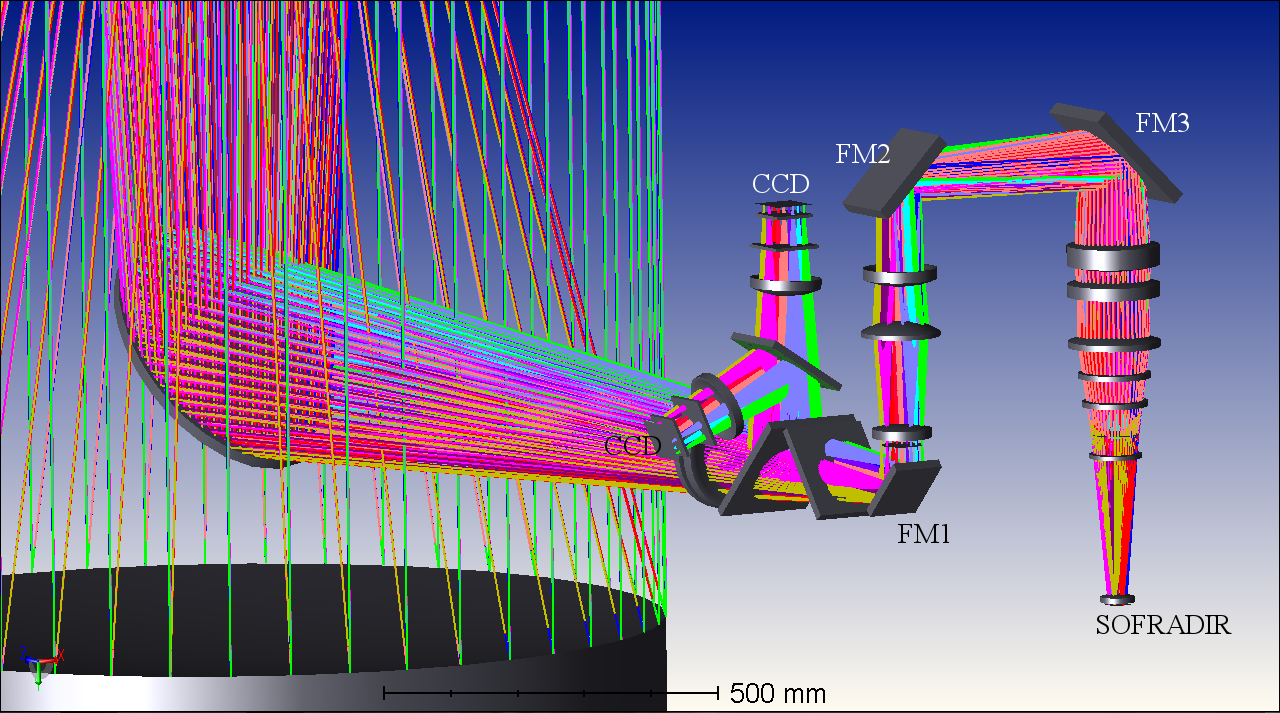
\includegraphics[width=0.7\linewidth]{figures/LAYOUT_3D.png}
\caption{A 3D view of the optics.}
\label{figure:optics-layout-3d}
\end{figure}

\begin{figure}
\centering
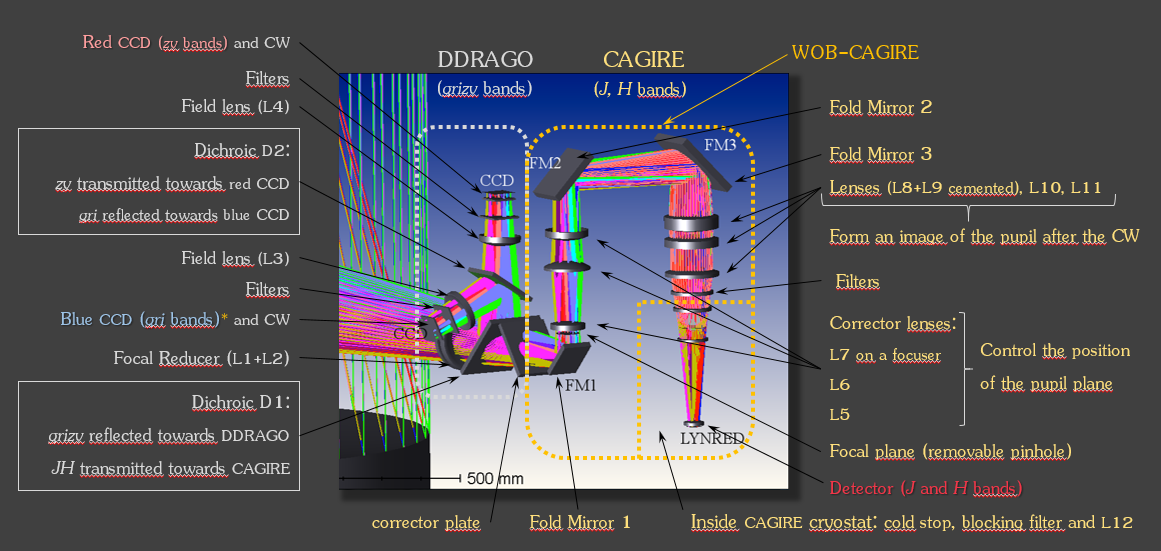
\includegraphics[width=1.0\linewidth]{figures/optics.png}
\caption{A schematic of the optics.}
\label{figure:optics-schematic}
\end{figure}

\begin{figure}
\centering
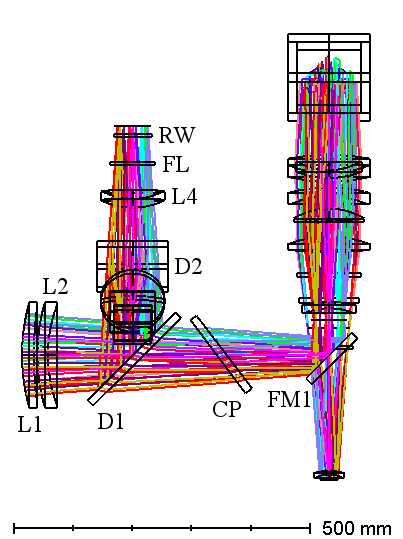
\includegraphics[width=0.3\linewidth]{figures/LAYOUT_lateral.png}%
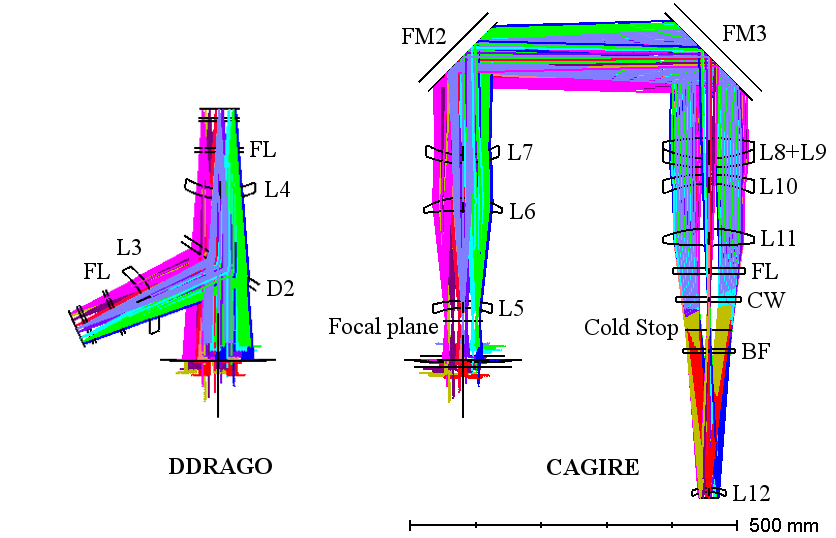
\includegraphics[width=0.7\linewidth]{figures/LAYOUT_front.png}
\caption{2D views of the optics. Left: a lateral view of the optics. Middle: an axial view of the DDRAGO optics for the blue and red channels. Right: an axial view of the WOB and CAGIRE optics.}
\label{figure:optics-layout-2d}
\end{figure}


\clearpage
\chapter{Telescope}

We are working to the CAD file “6960 GFT 2018-12-07\_R1.stp” provided by LAM. The DDRAGO and CAGIRE instruments are designed to mount at one of the Nasmyth focus of the COLIBRI telescope supplied by ASTELCO. Preliminary plans for the telescope (with nominal optics) are shown in Figures~\ref{figure:telescopeA} and \ref{figure:telescopeB}.

\begin{figure}
\begin{center}
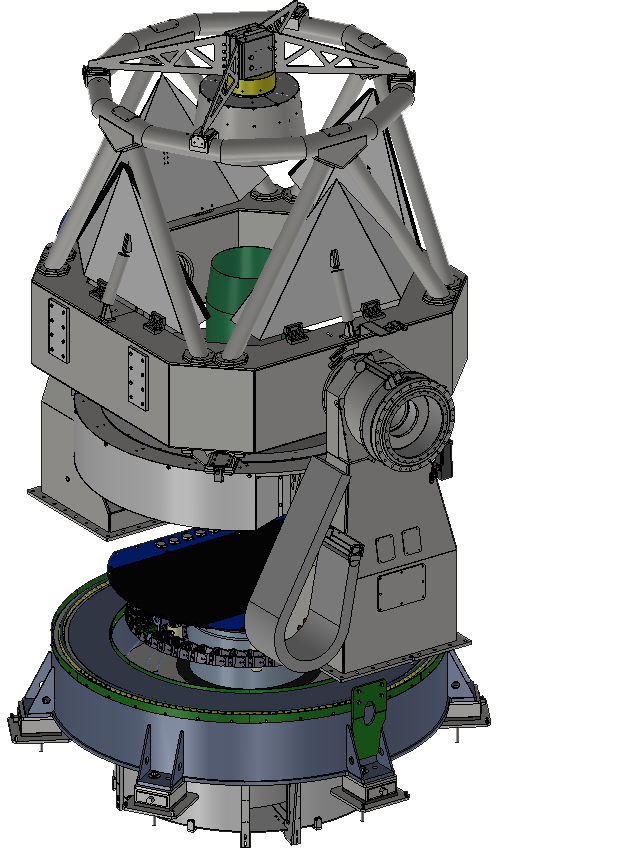
\includegraphics[width=\linewidth]{figures/Telescope-000.png}
\end{center}
\caption{The COLIBRI Telescope (6960 GFT 2018-12-07\_R1).}
\label{figure:telescopeA}
\end{figure}

\begin{figure}
\begin{center}
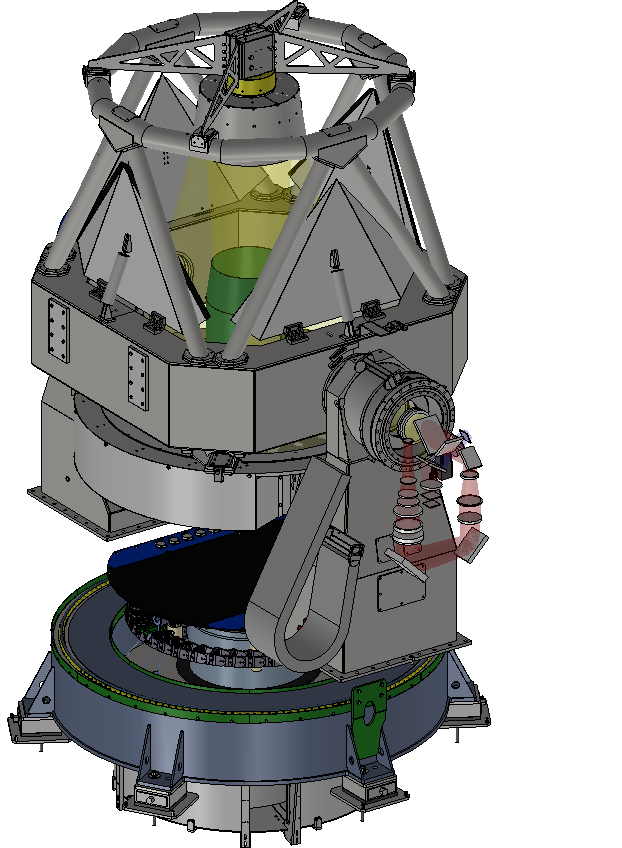
\includegraphics[width=\linewidth]{figures/Telescope-DD-Cg-Optics-000.png}
\end{center}
\caption{The Nasmyth Focus of the COLIBRI Telescope with DDRAGO, WOB and Cagire optical components.}
\label{figure:telescopeB}
\end{figure}

%\TODO{Confirm telescope interface with LAM.}

%We currently do not have a formal interface specification with the telescope. Therefore, our interface is designed according to our understanding of the telescope preliminary design. This is obviously unsatisfactory, and this uncertainty must be resolved quickly.

The definition of the interface with the telescope is defined by the derotator drawing provided by Astelco. The derotator flange is at a distance of 1.4384~m from the optical axis of M1 and M2 (Figure~\ref{figure:telescopeC}). The instrument is secured to the flange by eight M12 bolts with nuts whose centers are equally spaced on a circle of diameter 368~mm. 

The reference origin of the instrument for structural design is at the intersection of the optical axis and the derotator flange. Also, the derotator range angles of operation between $-65$° to $+65$° have been checked about possible mechanical interference with the instrument. The instrument at the derotator is free of interference with the derotator and the telescope.

\begin{figure}
\begin{center}
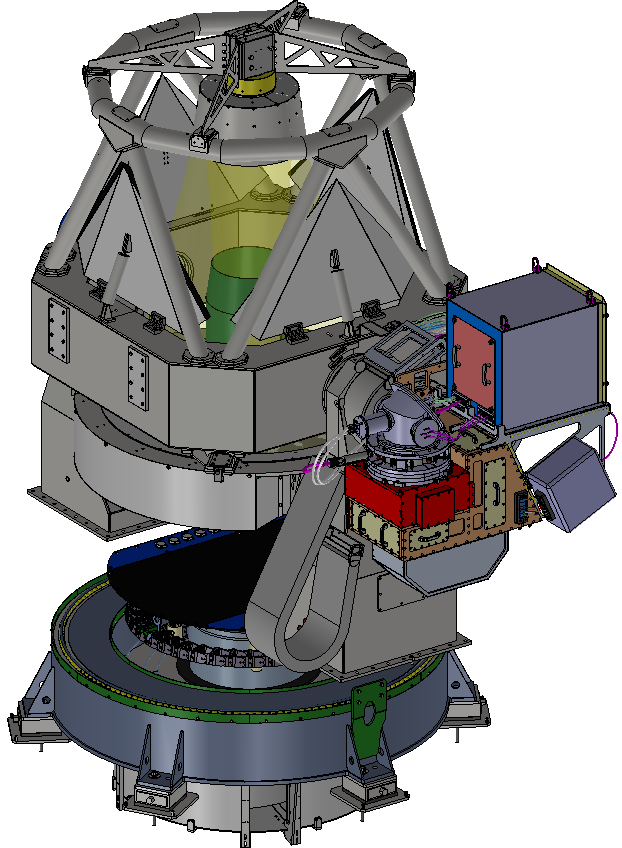
\includegraphics[width=\linewidth]{figures/Telescope-DD-Cg-Optics-Mechanics-000.png}
\end{center}
\caption{Instrument mounted at the derotator in the telescope.}
\label{figure:telescopeC}
\end{figure}

\clearpage
\chapter{Support Structure}

\section {General methodology}

The mechanical design of the support structure for DDRAGO and the WOB is based on the work done for the interim instrument DDRAGUITO. The design guidelines were:

\begin{itemize}
\item The structural plates are made out of high quality aluminium AluMold F500 (although an equivalent 7000-series alloy could be substituted if need be). This is important to achieve a compact instrument with the required stiffness.
\item Large and continuous plates can be manufactured with cut-outs where necessary, in order to give stiffness or to reduce mass.
\item The plates will be attached to each other using M8 bolts. A manufacturing tolerances for the holes of 0.500 micrometers is good enough to guarantee the feasibility for assembling the structure and the subsystems.
\item Flat surfaces on the structural plates can be used for bolting the optomechanics components. Threaded inserts are required between the structure and the optomechanics supports.
\item The support structure requires removable covers to allow the installation and calibration of all optomechanical and electronic components, however, these removable plates are considered not structural.
\end{itemize}

Figure \ref{figure:SSsubsystems} shows the components that need to be supported by the Support Structure, and Figure \ref{figure:SS} shows the complete Support Structure of DDRAGO.

\begin{figure}
\centering
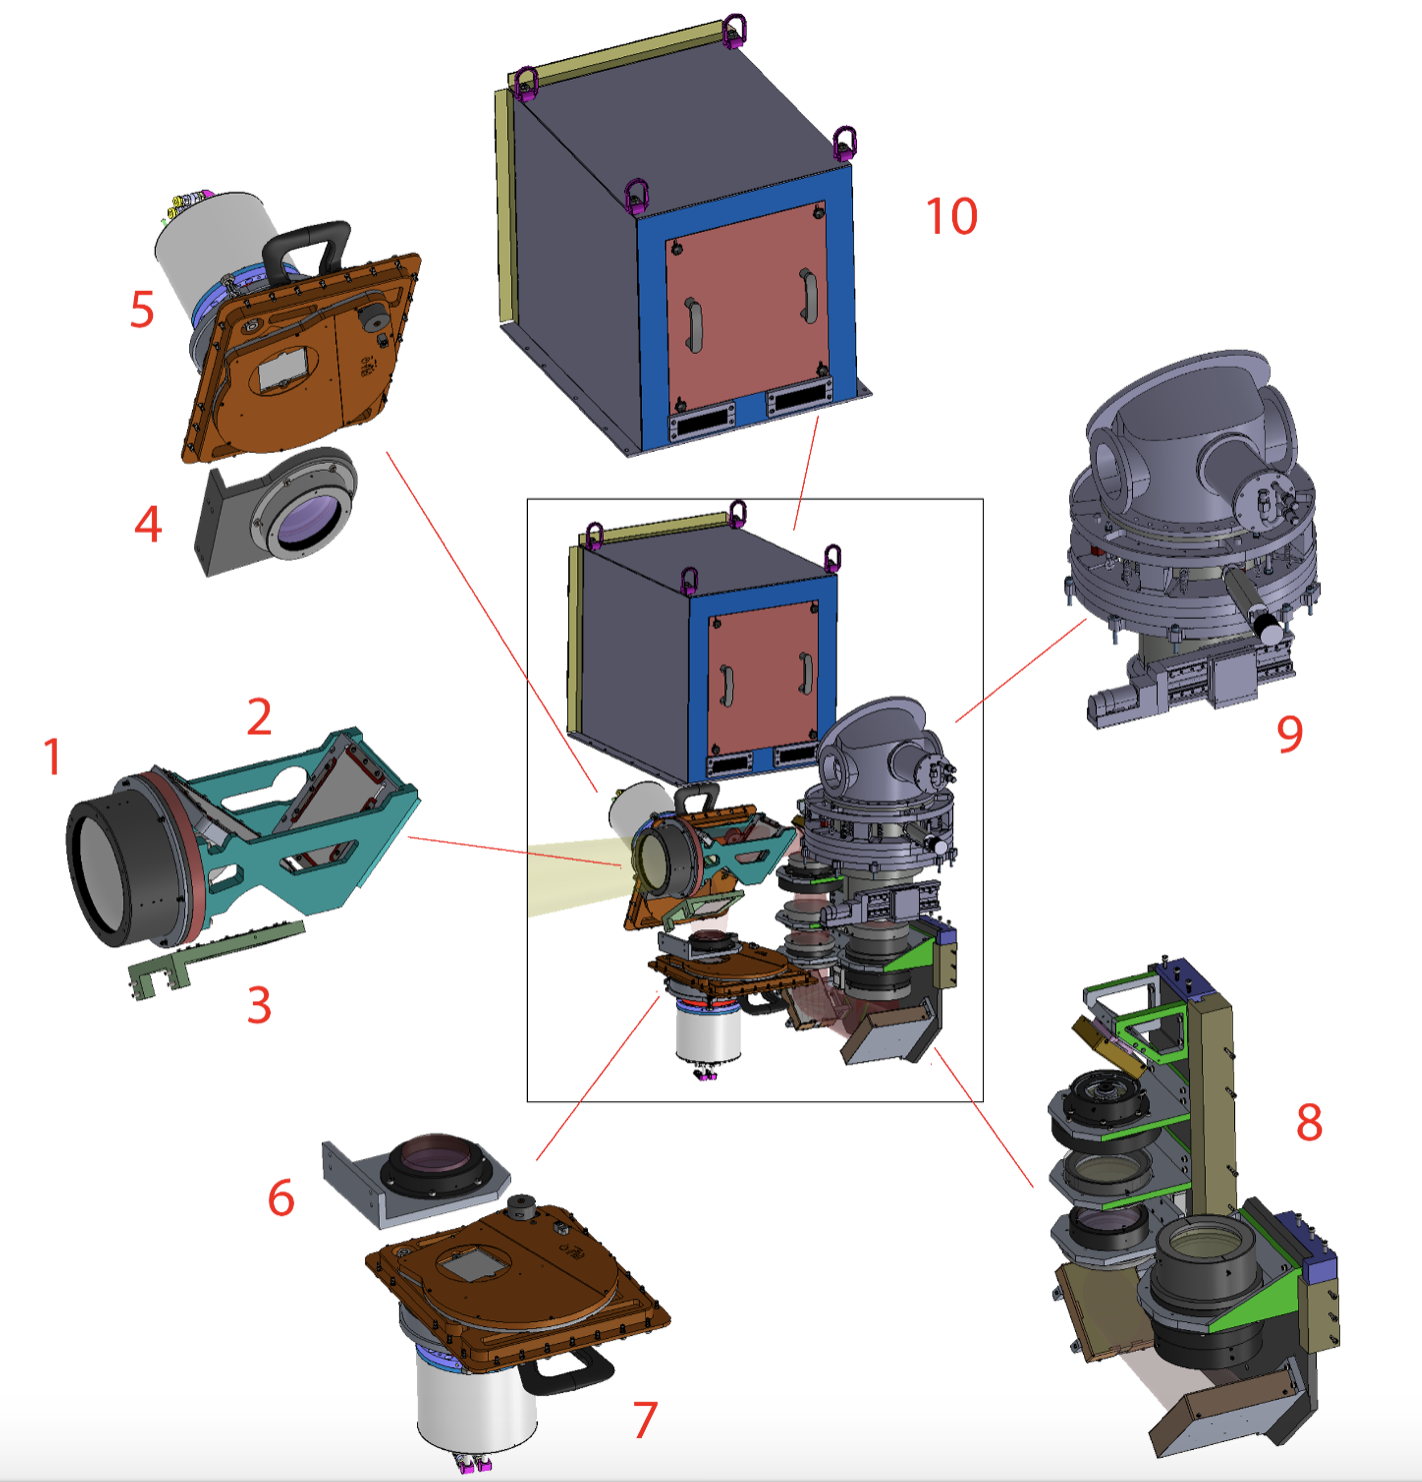
\includegraphics[width=1.0\linewidth]{figures/SSsubsystems.png}
\caption{Components supported by the DDRAGO Support Structure: (1) L1L2 barrel, (2) D1 and CP module, (3) D2 support, (4) L3 bracket, (5) blue detector with Tip/Tilt mechanism, (6) L4 bracket, (7) red detector with Tip/Tilt mechanism, (8) Warm Optical Bench, (9) CAGIRE cryostat, and (10) CAGIRE close electronics.}
\label{figure:SSsubsystems}
\end{figure}

\begin{figure}
\centering
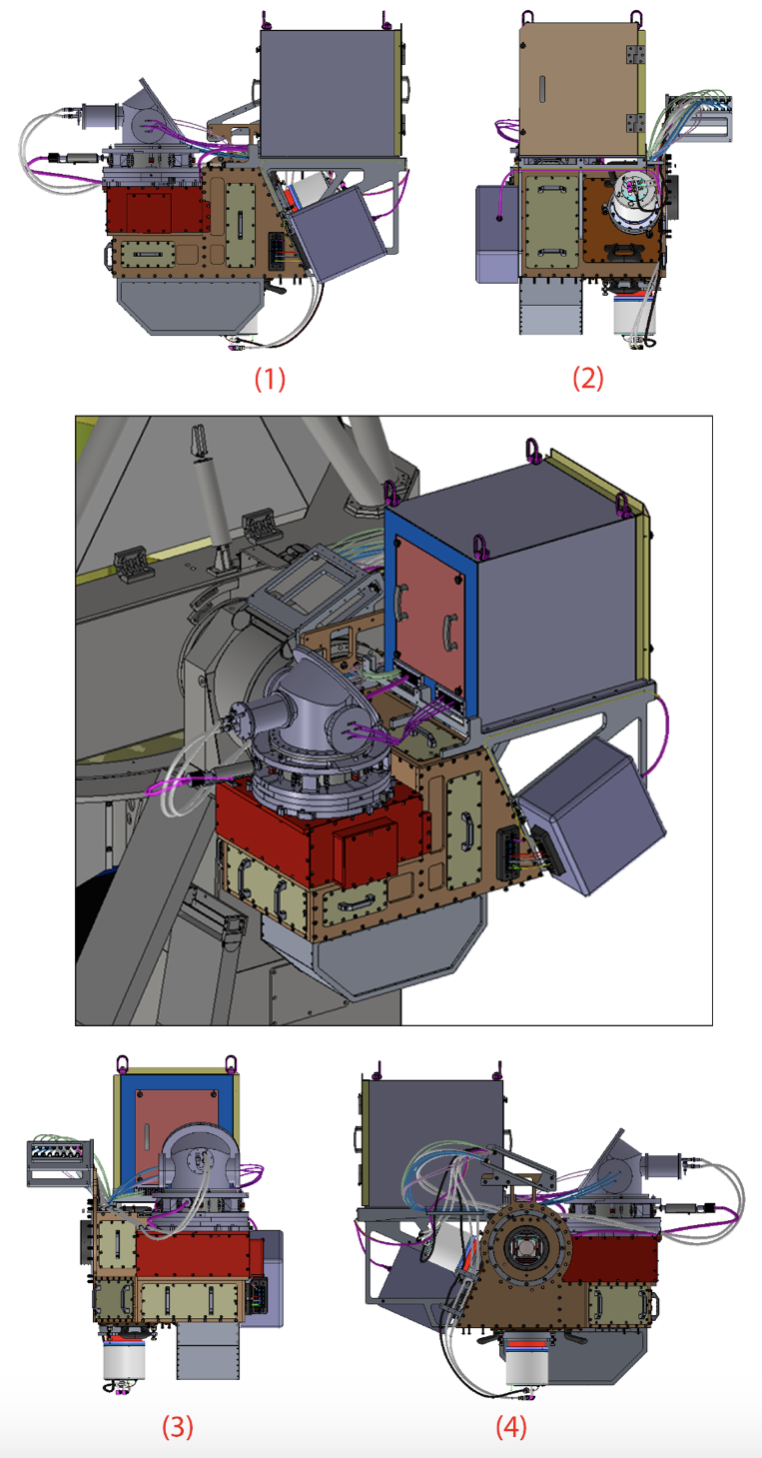
\includegraphics[width=0.7\linewidth]{figures/SS.png}
\caption{DDRAGO Support Structure. We show a frontal view (1), the view from DDRAGO detectors (2), the view from the Cryostat side (3) and the view from the telescope derotator (4).}
\label{figure:SS}
\end{figure}

There are three removable eyebolts for lifting the instrument with the harness. Two will be placed in structural plate FP3 and one in the cryostat support. The eyebolts are McMaster part number 3040T15.

\clearpage

\section{Support Structure parts}

The Support Structure plates are classified as: fixed plates (DD-ME-SST-Pn), removable plates (DD-ME-SST-RPn), cryostat plates (DD-ME-SST-CYS-Pn), close electronics (DD-ME-SST-CEn), and cable wrap support (DD-ME-SST-CWS-n), where n refers to the plate number. The fixed plate DD-ME-SST-P1 is the interface between the telescope derotator and the instrument. Figures \ref{figure:SSfixedplates} and \ref{figure:SSexploded} show different views of the fixed plates and the cable wrap support. Alignment of the instrument with the derotator is achieved with the centering ring (DD-ME-SST-CTR). This is 50 {\micron} undersized with tolerance h5 and so with the H6 tolerance on the derotator, hence the final margin will be between 60 and 103 \micron.

The Support Structure does not have any adjustments to refine the centering of the instrument respect the telescope due the fit tolerances between them.  To guarantee the mechanical alignment of the instrument with the derotator axis, the main structure, optmechanical barrels, and all reference surfaces are going to be calibrated respect the centering ring (DD-ME-SST-CTR). The Support Structure of DDRAGO is about 90 × 68 × 60 cm and, as in the interim instrument DDRAGUITO, this verification process of alignment, will be validated by the use of the Mitutoyo 7106 coordinate-measuring machine (range up to 100 × 70 × 60 cm) and others metrology tools in the IA workshops. 

The fixed plate DD-ME-SST-P1 is the mechanical interface to the telescope derotator. It also supports the optomechanical barrel for the doublet L1+L2, the optomechanics for L3, L4 D1, CP and D2 support, and the cable wrap (DD-ME-SST-CWSP), as shown in Figure \ref{figure:SSholds}. The latter is divided in the cable wrap support (DD-ME-SST-CWS1) and the cable support guides (DD-ME-SST-CG1/2).

The geometrical tolerances of the centering ring and fix plate P1 will be checked. If the components do not comply specifications, they will be corrected by remachining until achieving tolerances. The use of shimming is not part of the mounting process of DDRAGO.

\begin{figure}
\centering
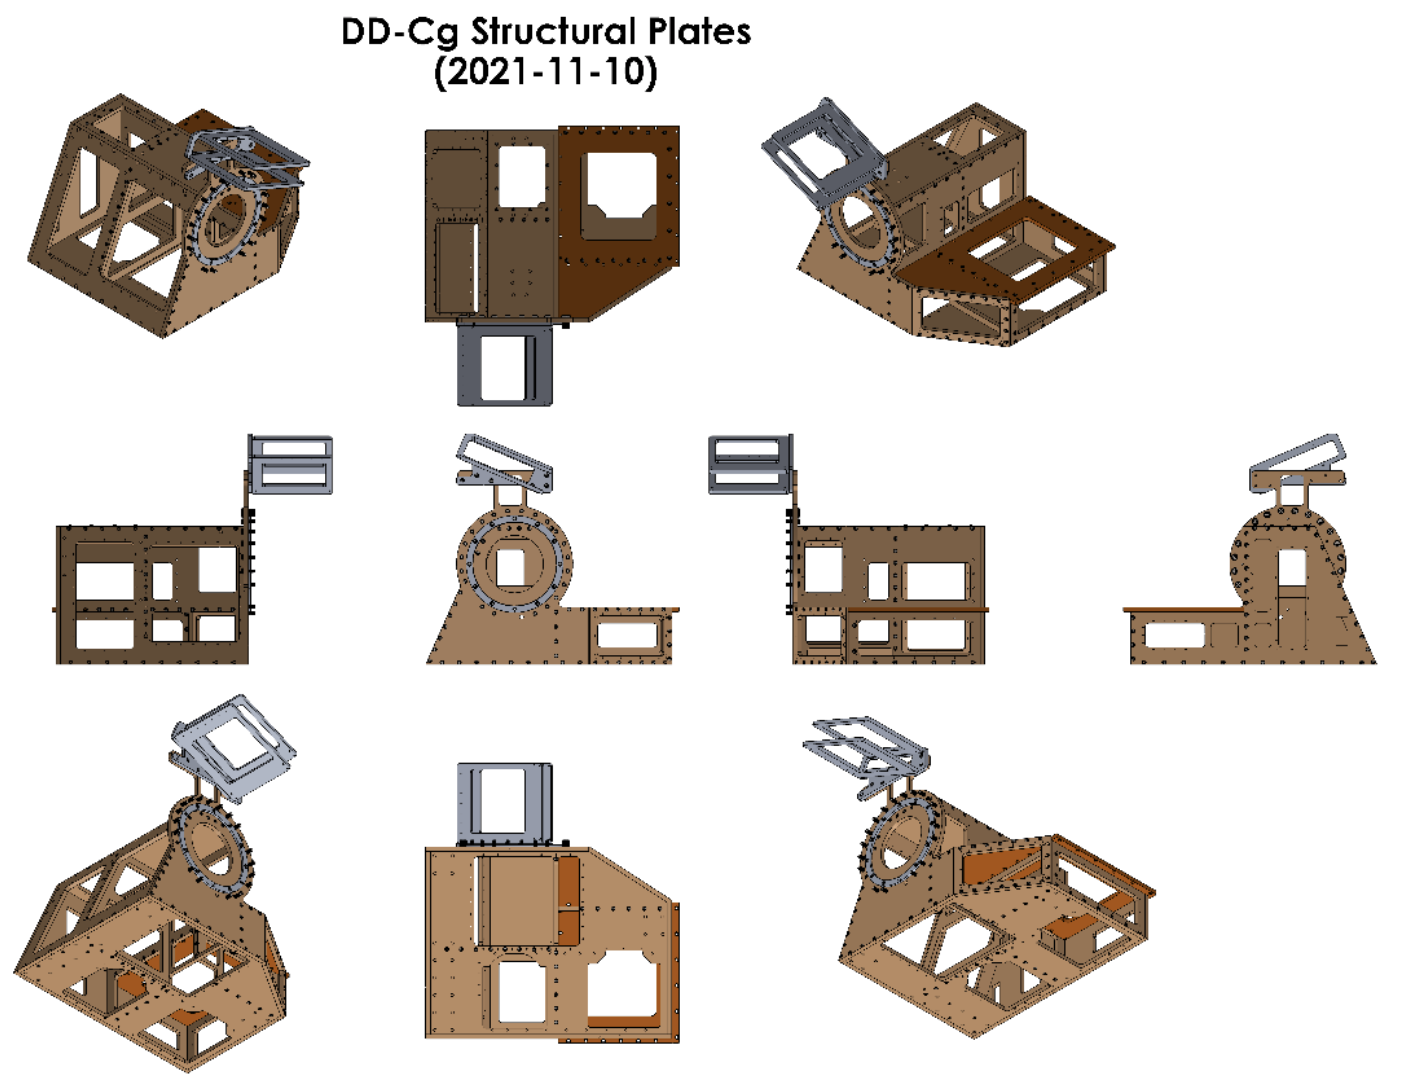
\includegraphics[width=1\linewidth]{figures/SSfixedplates.png}
\caption{Views of the fixed plates and the cable wrap support.}
\label{figure:SSfixedplates}
\end{figure}

\clearpage

\begin{figure}
\centering
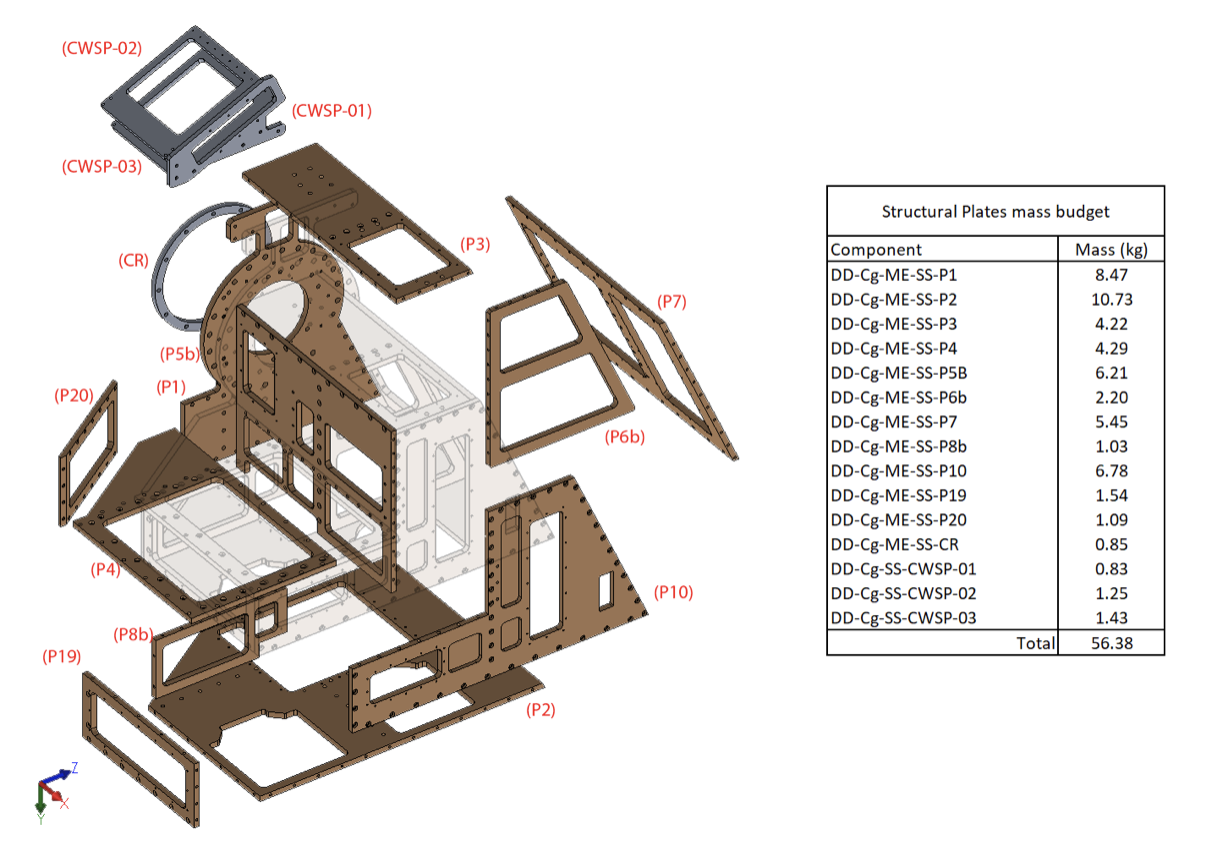
\includegraphics[width=1\linewidth]{figures/SSexploded.png}
\caption{Support Structure exploded view.}
\label{figure:SSexploded}
\end{figure}

\begin{figure}
\centering
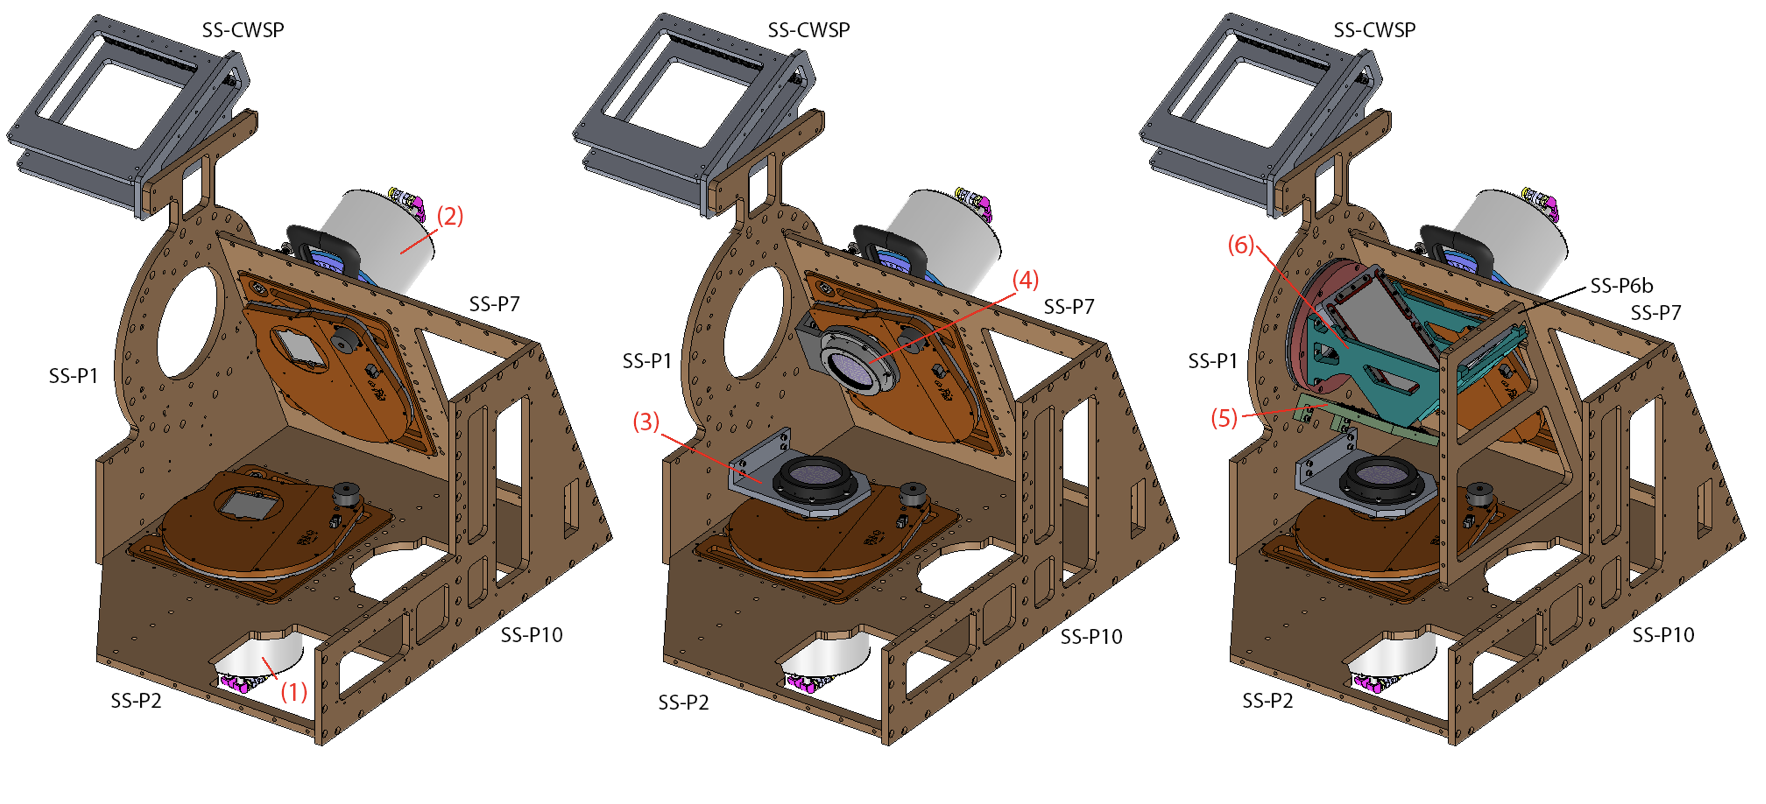
\includegraphics[width=1\linewidth]{figures/SSholds.png}
\caption{Plates at the Support Structure that hold red detector with Tip/Tilt mechanism (1), blue detector with Tip/Tilt mechanism (2), L4 bracket (3), L3 bracket (4), D2 support (5), and D1 and CP module (6).
}
\label{figure:SSholds}
\end{figure}

Figure \ref{figure:SSremovable} shows different views of the removable plates. Each allows access to different subsystems, as follows:
\begin{itemize}
\item RP1 and RP2 at the back of the WOB allow access useful for watching and guiding the integration of the WOB into the Support Structure.
\item RP3 allows access to the L3 optomechanics.
\item RP4 allows access to the D1/CP module and the D2 support.
\item RP14 allows access to the WOB for lateral adjustments of FM1 and to the shutter on OML5.
\item RP15 allows access to L8-L11 barrel.
\item RP16 allows acces to the WOB for top adjustments of FM1.
\end{itemize}

The CAGIRE Close Electronics is placed at the needed position to help balancing the instrument at the telescope derotator. It weighs 63 kg and it will have a position tolerance of 1 centimeter. Figure \ref{figure:SScloseelec} shows the support for the Close Electronics.

In order to avoid stray light entering the instrument, the cover plates have slits, where possible. Where not, it will be sealed with dark UV-Resistant Glass Sealant, Silicone, (McMaster 6937T92). This sealing is going to be used inside the joints of the WOB cover, and it does not affect accessibility because it shall be removed as a unit.

\begin{figure}
\centering
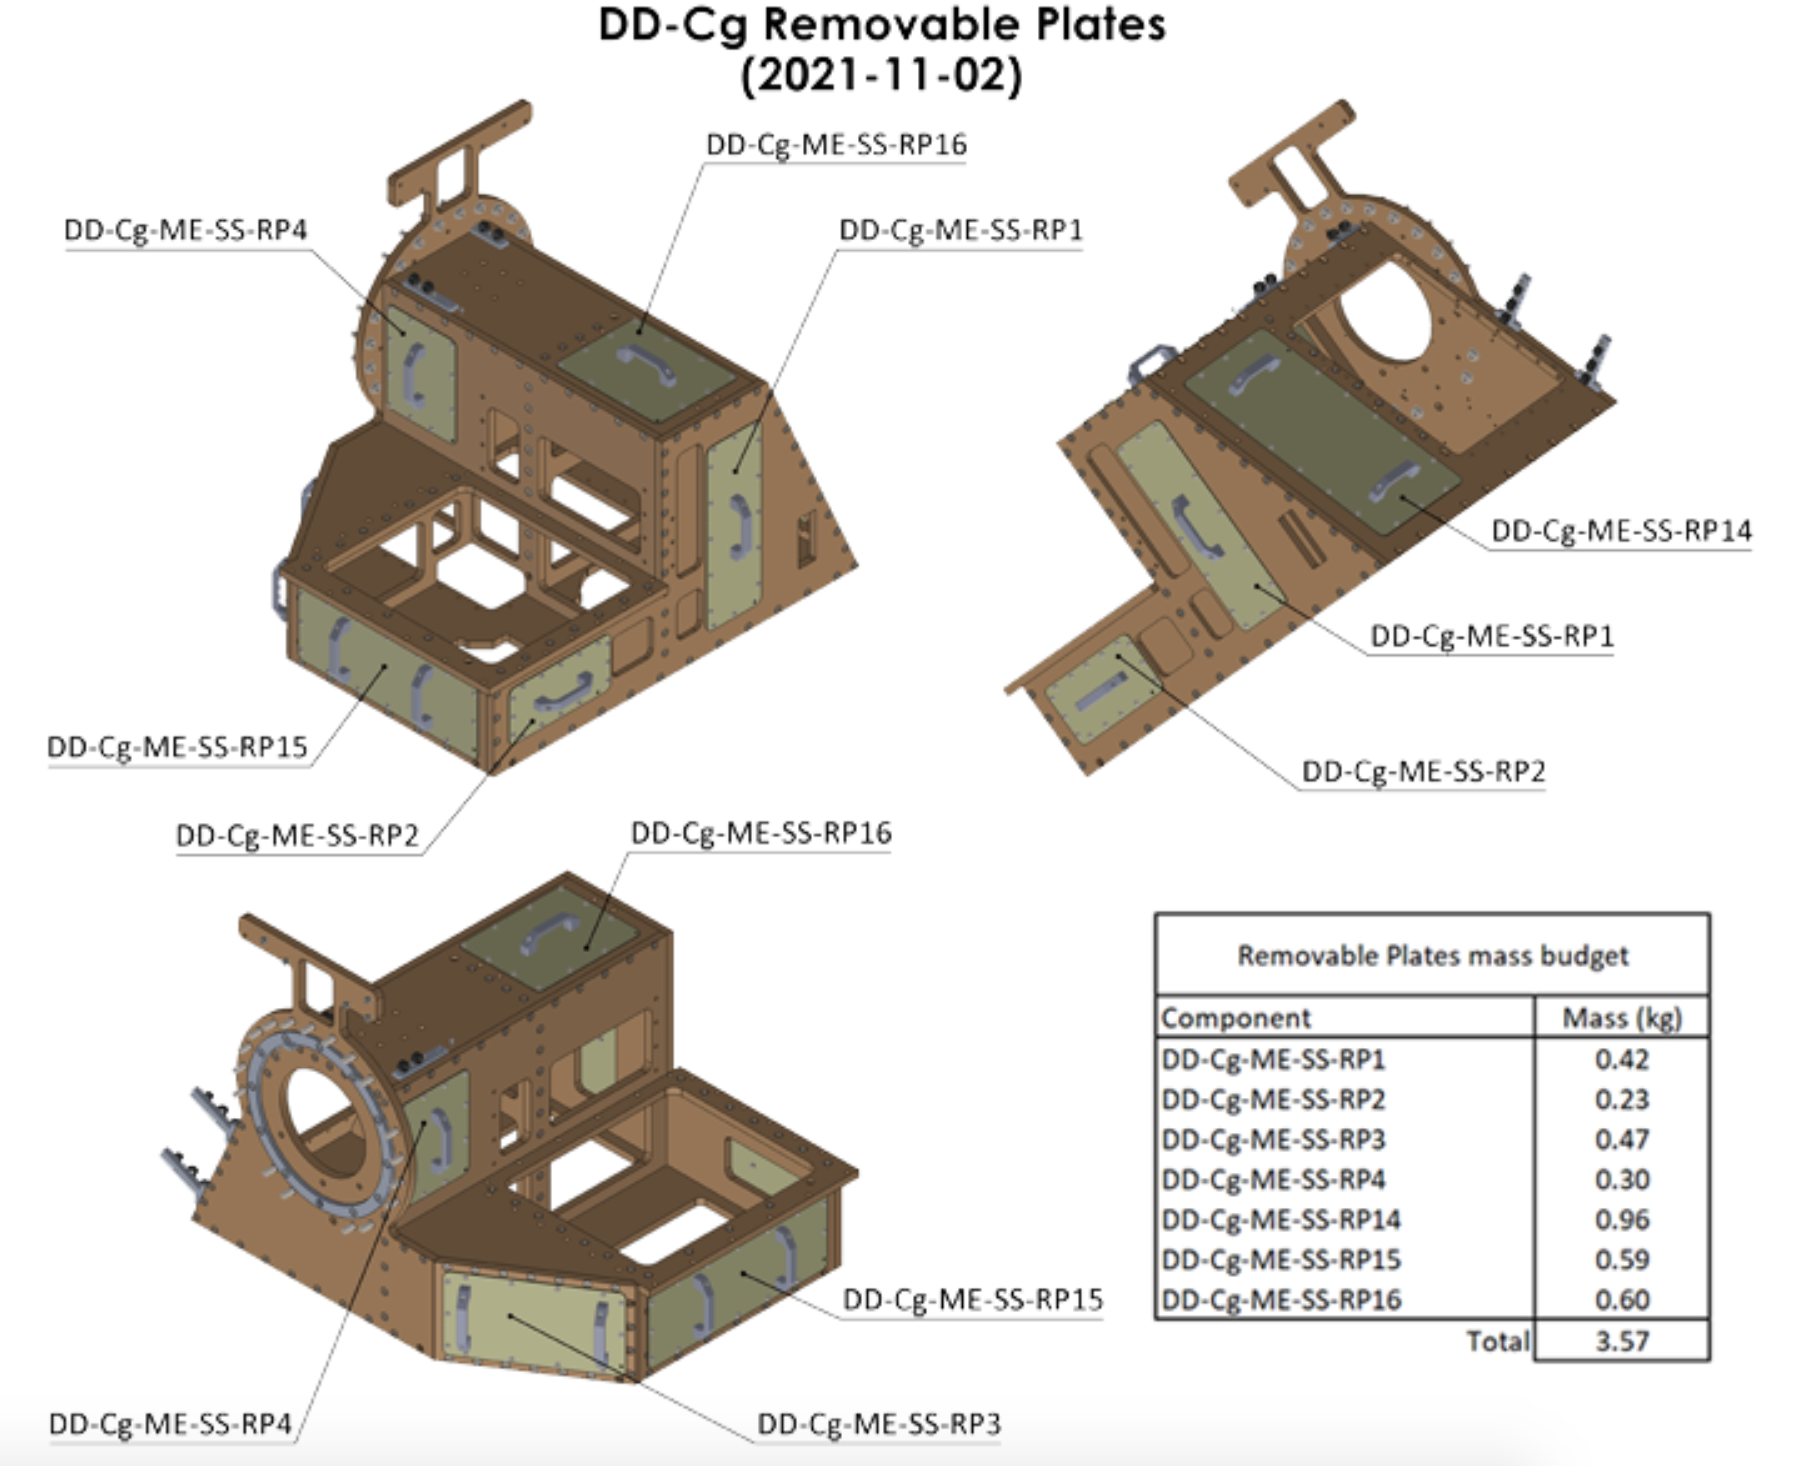
\includegraphics[width=1\linewidth]{figures/SSremovable.png}
\caption{Views of the removable plates.}
\label{figure:SSremovable}
\end{figure}

\begin{figure}
\centering
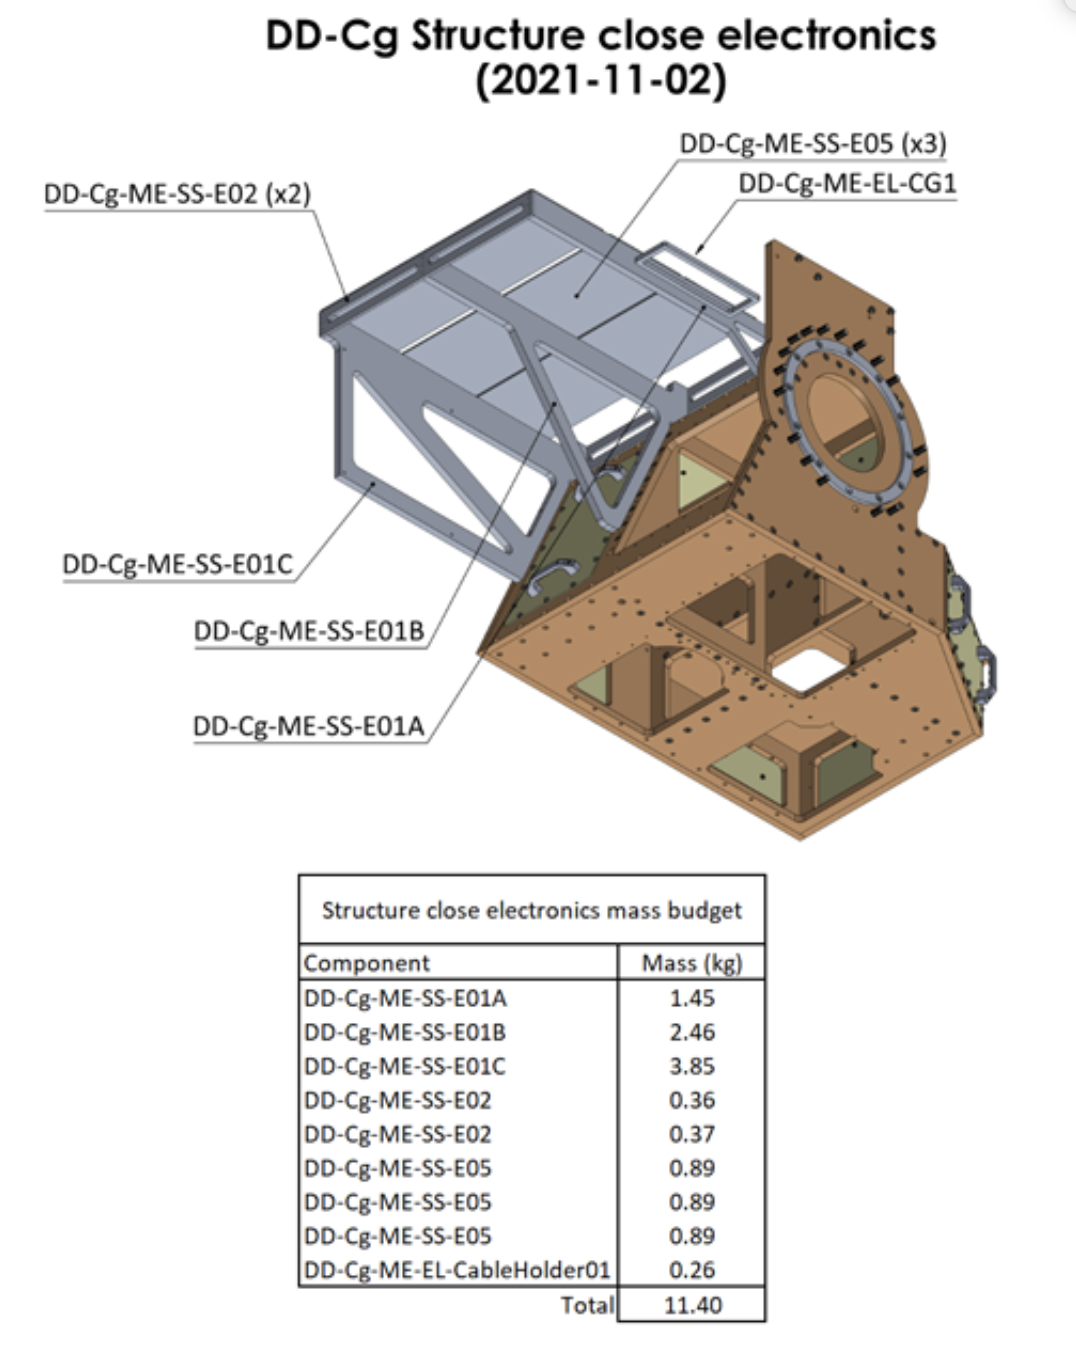
\includegraphics[width=1\linewidth]{figures/SScloseelec.png}
\caption{Close Electronics support.}
\label{figure:SScloseelec}
\end{figure}

\clearpage

\section{Cryostat support}

The design of the Support Structure considered an independent surface of reference for attaching the Cryostat. The requirement of integrability to the Support Structure in a rigid manner is fulfilled (see Finite Element Analysis results in Section 10). The mechanical envelope, including movements, rotations and filters translation, is free of mechanical interferences.

The integration of the Cryostat to the Support Structure requires removing the cryostat plate DD-ME-SST-CYSP5B at the beginnig of the process, to allow free access to the Crysotat with the filters stage installed. The plate must be reinstalled before placing the Cryostat at this surface of reference.

Figures \ref{figure:SScryo} and \ref{figure:SScryoexploded} show views of the support structure for the Cryostat.

\begin{figure}
\centering
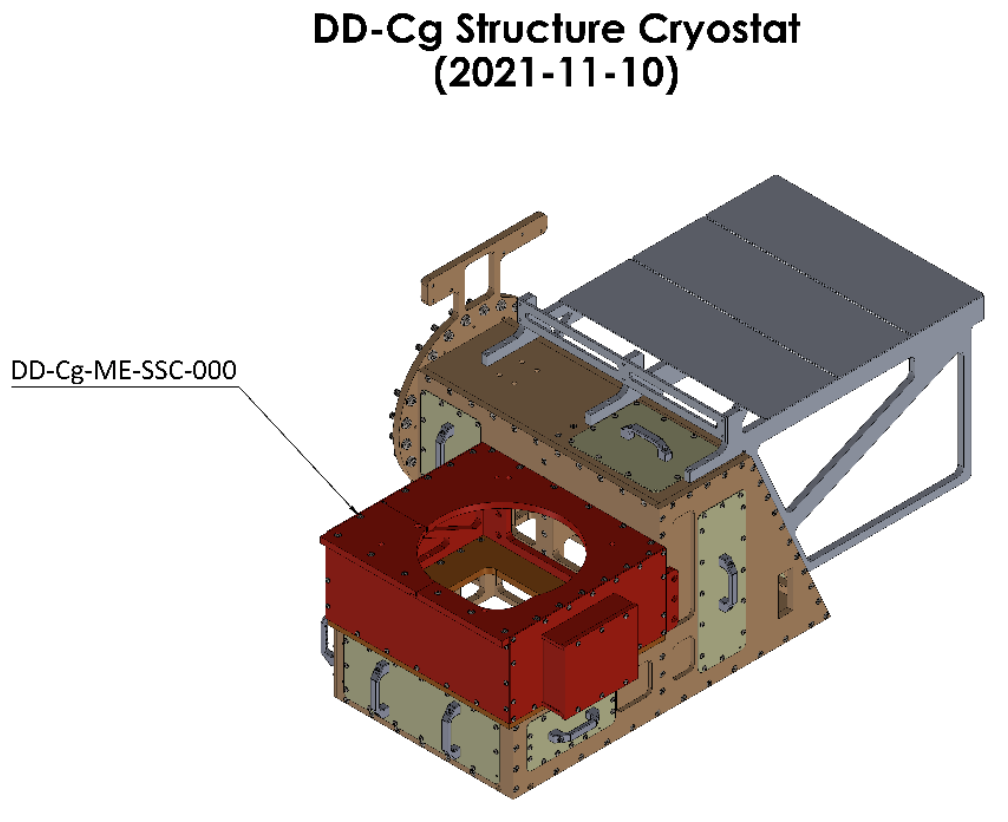
\includegraphics[width=0.7\linewidth]{figures/SScryo.png}
\caption{Cryostat support structure.}
\label{figure:SScryo}
\end{figure}


\begin{figure}
\centering
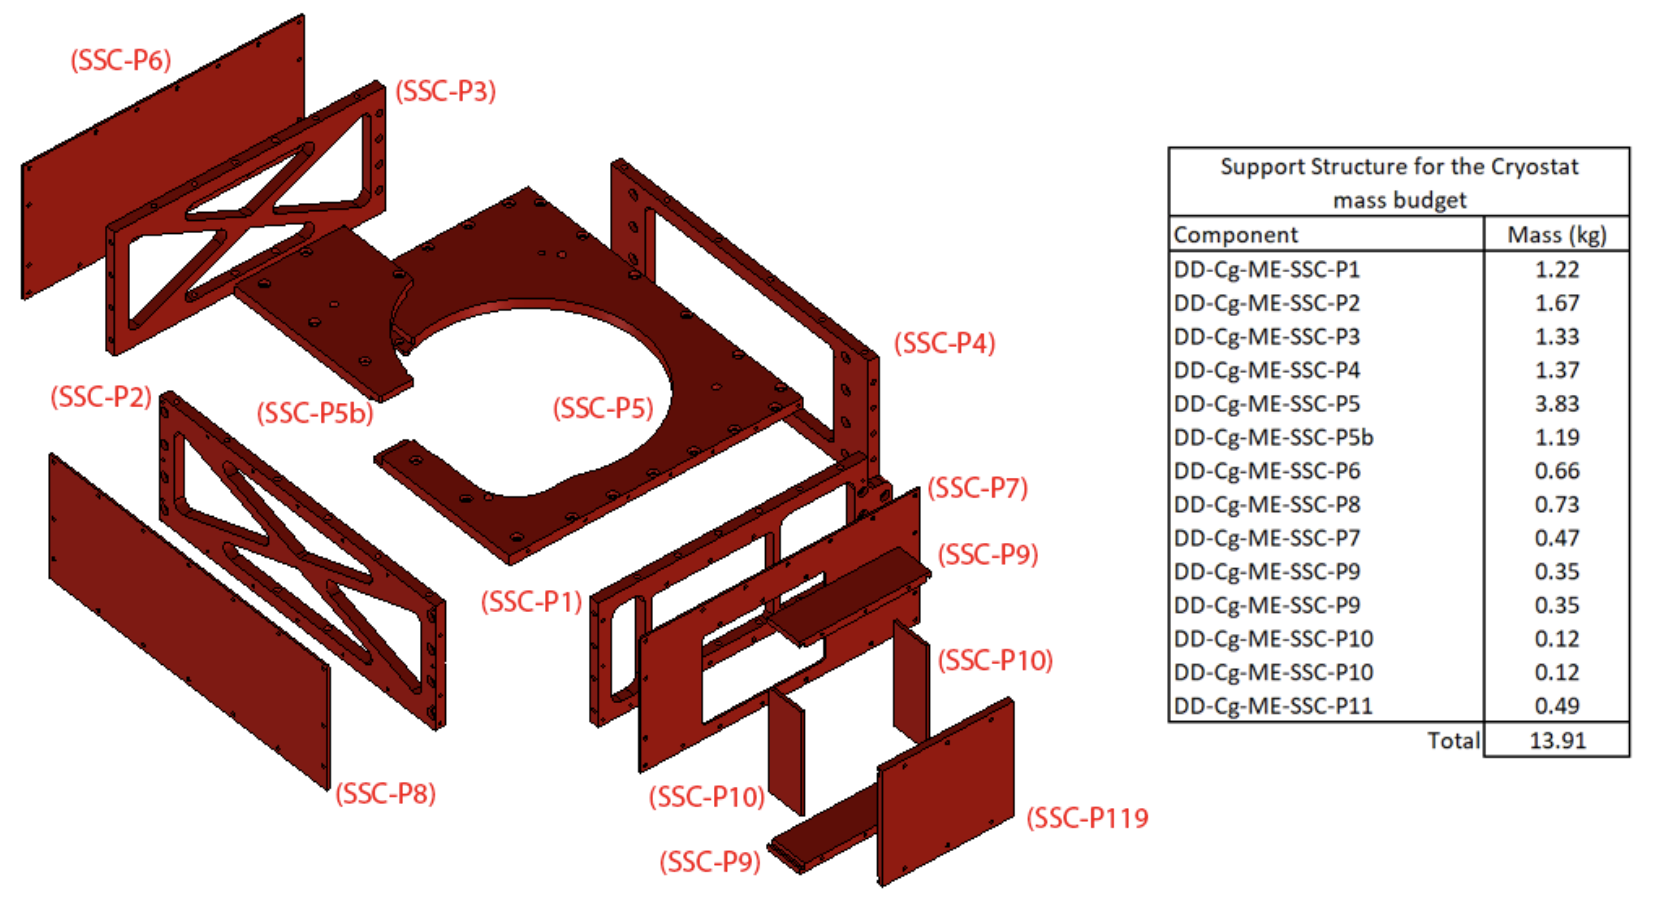
\includegraphics[width=0.8\linewidth]{figures/SScryoexploded.png}
\caption{Cryostat support structure exploded view.}
\label{figure:SScryoexploded}
\end{figure}

\section{WOB cover}

The WOB cover has the function of protecting the WOB and the FM2 and FM3 subsystems (Figure \ref{figure:SSwobcover}). It is totally removable from the Support Structure without the need of disassembling it. It was designed as a non-structural component with low weight. Once the instrument is on the telescope the WOB cover can be removed to adjust the Fold Mirrors, if required.

The contact surfaces between the fixed plate DD-Cg-ME-SS-P2 and the WOB cover plates will have foam as light traps (Chemical-Resistant Viton Fluoroelastomer Foam Sheets and Strips, McMaster 1669N105).

\begin{figure}
\centering
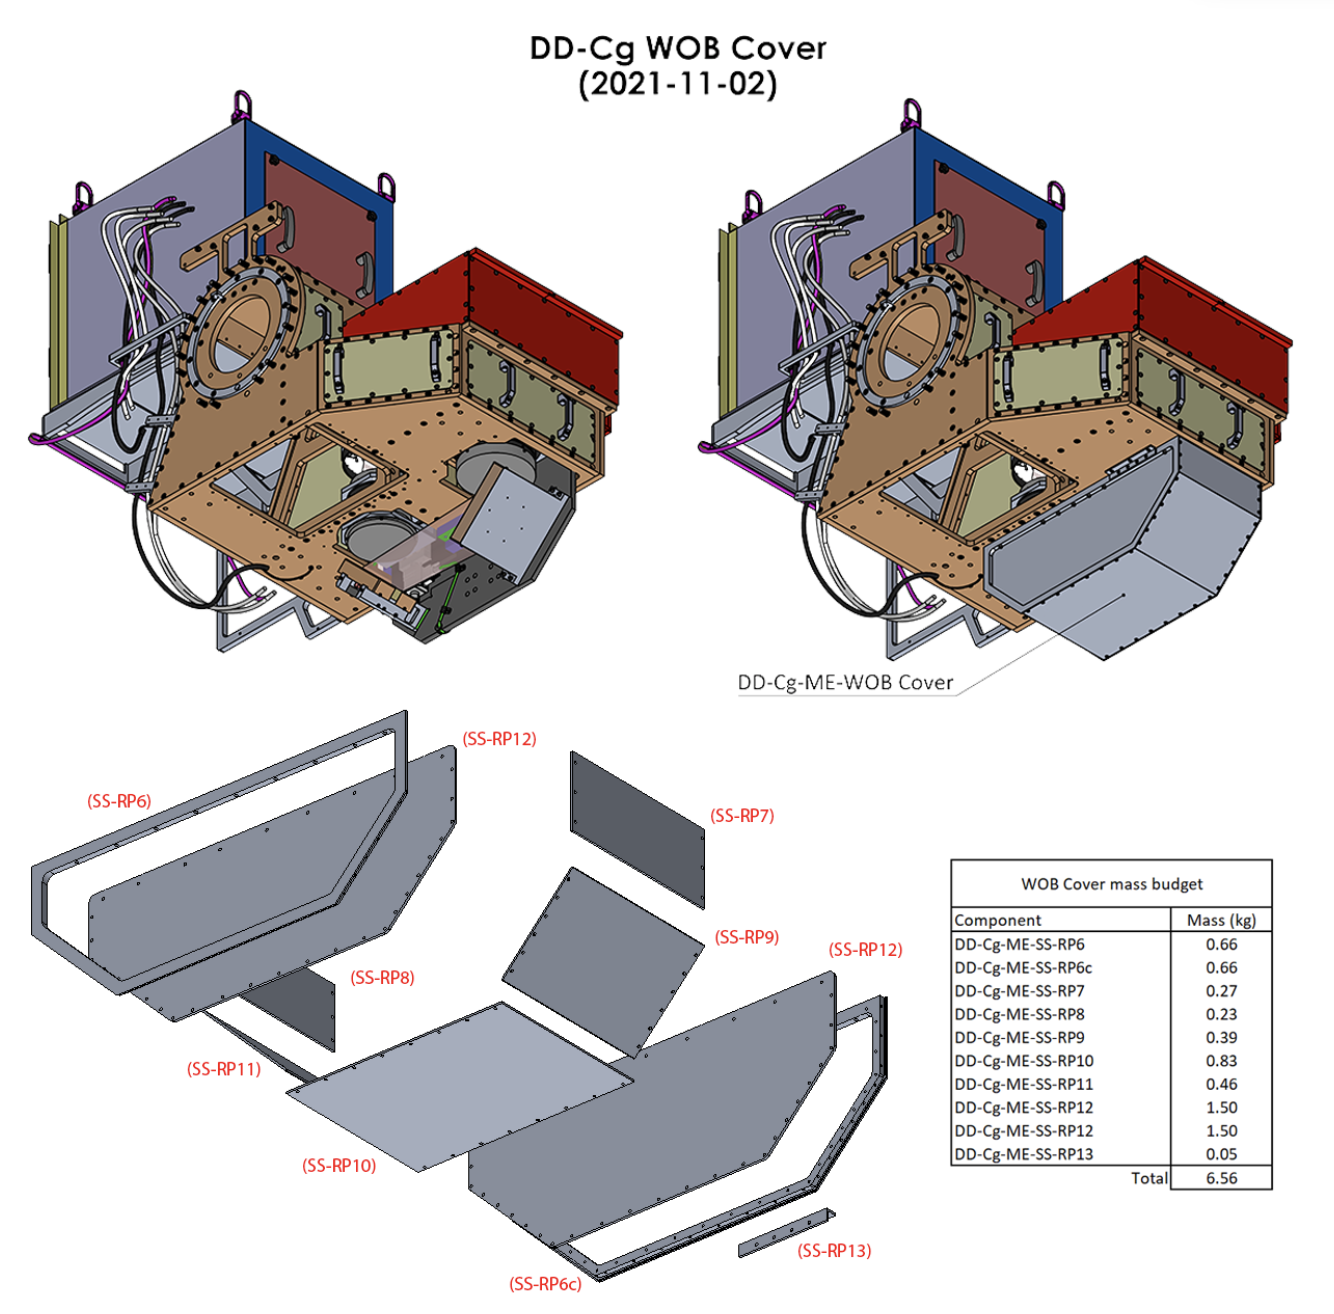
\includegraphics[width=1\linewidth]{figures/SSwobcover.png}
\caption{WOB cover.}
\label{figure:SSwobcover}
\end{figure}

\section{Counterweights}


\begin{figure}
    \centering
    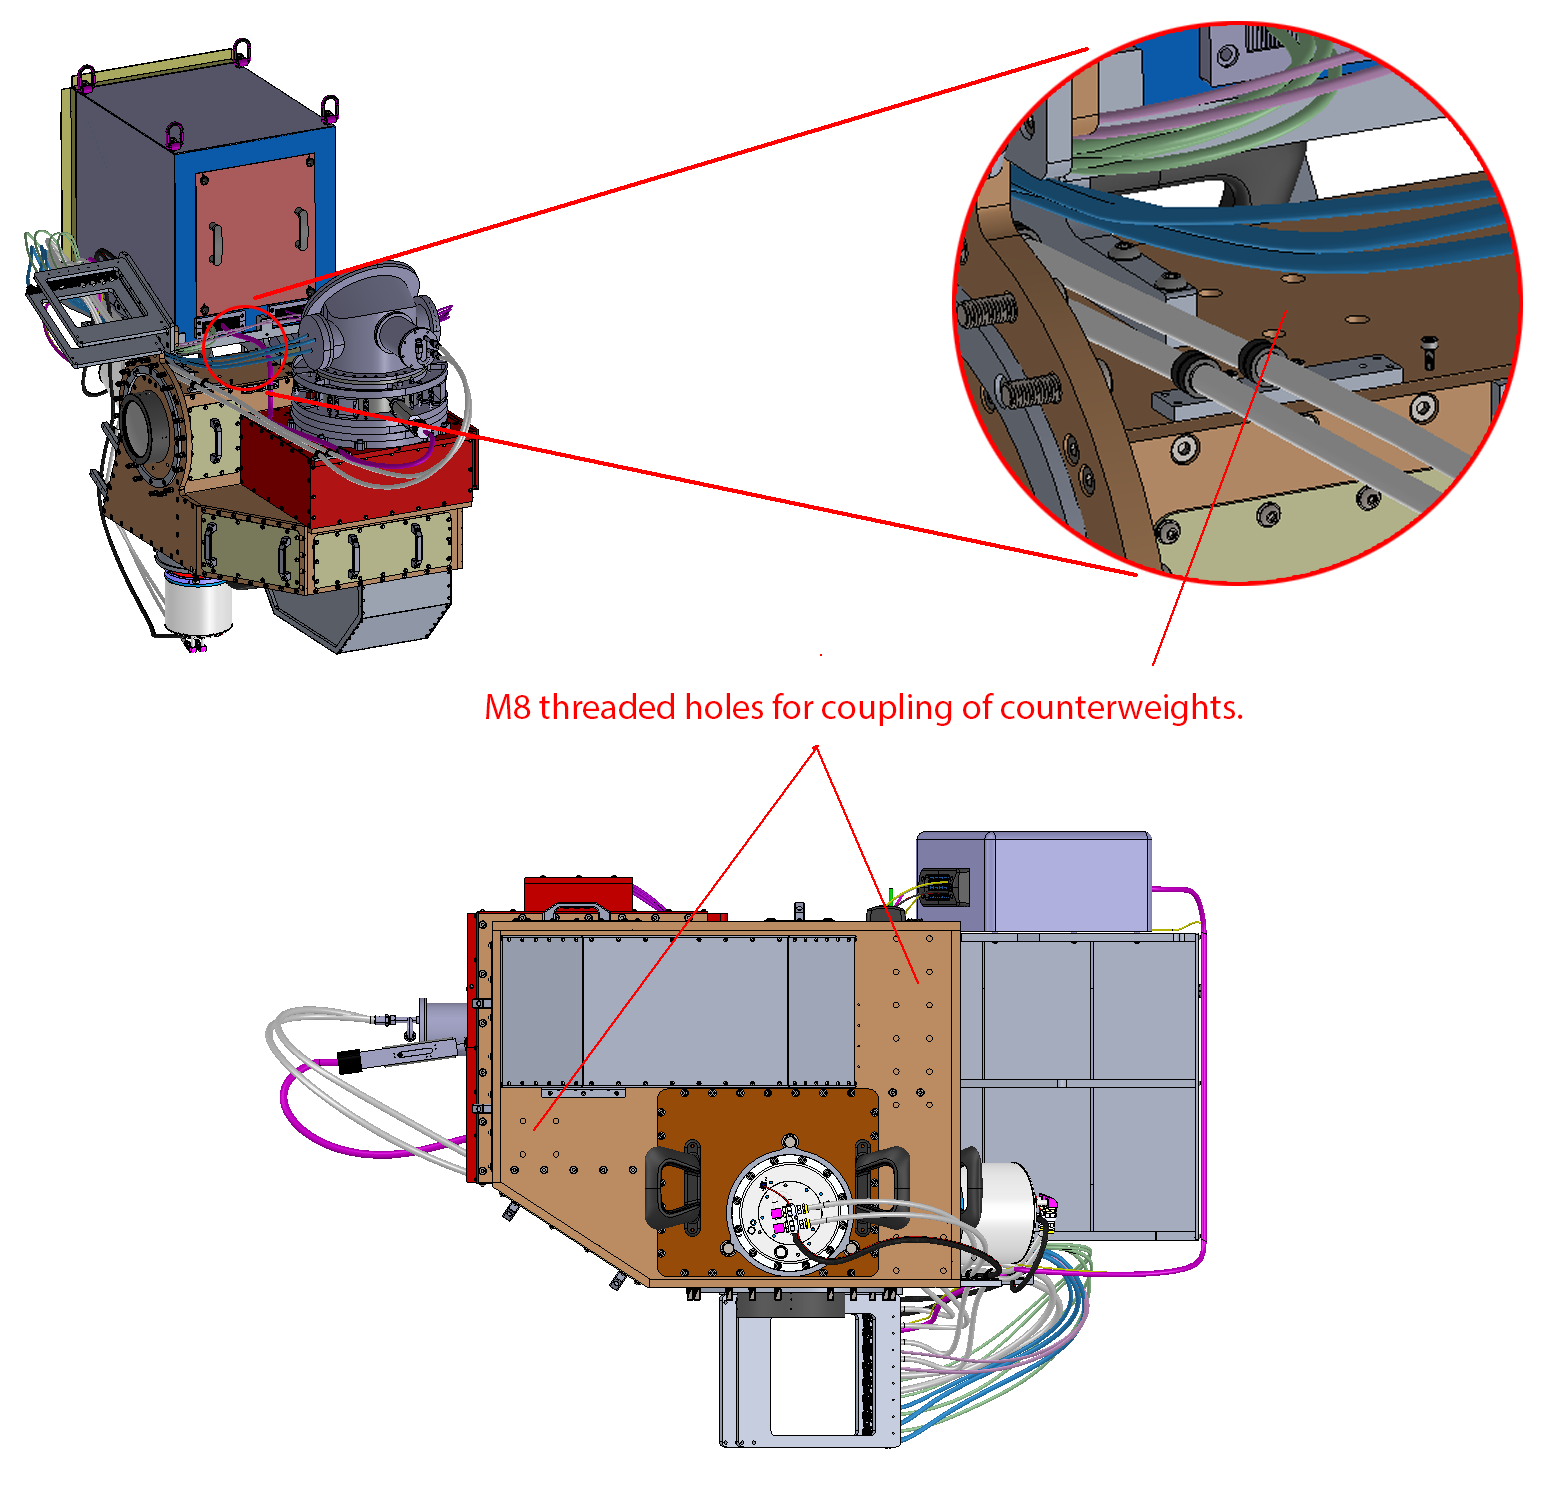
\includegraphics[width=0.7\linewidth]{figures/DD-Cg-CounterWeights.png}
    \caption{Attachment points for the counterweights}
    \label{figure:counterweights}
\end{figure}

The position of the center of mass of the MSU was optimized by moving the CAGIRE electronics, so the center of mass is close to the derotator axis. Additionally, when the instrument is finished, it will be possible to add counterweights to correct any imbalance.
The MSU design provides points for attaching counterweights on plates FP2 and FP3. See Figure~\ref{figure:counterweights}.

On plate FP2, there is room for counterweights of dimensions up to
$98 \times 96 \times 25$,
$100 \times 98 \times 25$ and 
$200 \times 100 \times 25$ mm.

On plate FP3, there is room for counterweights of dimensions up to
$200 \times 96 \times 25$ mm.

We will provide counterweights with different thicknesses, made from cold-rolled steel, and the adequate holes patterns so they can be used according to the balance needed for the instrument.


\clearpage


%\section{Design}

%\TODO{Lifting eyes on the SS?}

%\TODO{Describe support for RET1.}

%\subsection{General Principles}

%The preliminary design of the support structure for DDRAGO and CAGIRE instruments is a refinement of the design we presented at the Conceptual Design Review in June 2016 and Preliminary Design Review in February 2017. The science group, the optical designers, and mechanical designers worked together to refine this design through several iterations.

%In our experience, for a compact instrument one of the best options for the support structure is using plates. This gives excellent stiffness but also allows us to use pin-holes in the plates as references for placing optical components. We built the warm part of the RATIR instrument according to these ideas, and the result was successful.


%Our design uses 15 mm thick plates of Alumold 500 (although an equivalent 7000-series alloy could be substituted if need be). Alumold 500 is suitable for precision machining. We have used relatively large and continuous plates, with cut-outs where necessary, to give stiffness. The plates will be attached to each other using M8 bolts and threaded steel inserts. The manufacturing tolerances for these holes is good enough to guarantee the feasibility for assembling the structure and the subsystems.

%The support structure has removable covers to allow the installation and calibration of all optical and electronic components of the instrument.

%\TODO{All removable plates need handles to ease their manipulation.}

%\subsection{Complete Support Structure}

%Figure~\ref{figure:alex-supported-components} shows the main components that are supported by the support structure.

%\begin{figure}[p]
%\begin{center}
%\includegraphics[width=\linewidth]{figures/alex-supported-components.jpg}
%\end{center}
%\caption[The Supported Components]{The Supported Components. 1: The red and blue detector mounts (DR-ME-OMBDET and DR-ME-OMRDET). 2: The D1 mount (DR-ME-OMD1). 3: The D2 mount (DR-ME-OMD2). 4: The L4 mount (DR-ME-OML4). 5: The L3 mount (DR-ME-OML3). 6: The CP mount (DR-ME-OMCP). 7-13: CAGIRE WOB optical mounts. 14: The DDRAGO close electronics (DR-CO-CE). The support structure also has to support the CAGIRE cryostat and close electronics and the various hoses and cables for the control systems.}
%\label{figure:alex-supported-components}
%\end{figure}

%\begin{figure}[p]
%\begin{center}
%\includegraphics[width=\linewidth]{figures/alex-complete.jpg}
%\end{center}
%\caption[The Complete Support Structure and the Components it Supports.]{The Complete Support Structure and the Components it Supports. (a--c) Transverse and lateral views of the support structure including all DDRAGO and CAGIRE components. (d) 3D view of the support structure including only the DDRAGO components. (e) 3D view of the support structure including all DDRAGO and CAGIRE components. The designs of the CAGIRE cryostat and close electronics are preliminary; we presume the final version of the close electronics will have a closed cabinet.}
%\label{figure:alex-complete}
%\end{figure}

%Figure~\ref{figure:alex-complete} shows the complete support structure and all of the supported components.

%\begin{figure}a
%\begin{center}
%\includegraphics[width=\linewidth]{figures/alex-ss-exploded.jpg}
%\end{center}
%\caption{The Support Structure Plates}
%\label{figure:alex-ss-exploded}
%\end{figure}

%Figure~\ref{figure:alex-ss-exploded} shows the support structure plates. We classify the plates as fixed (DR-ME-SS-FP$n$), removable (DR-ME-SS-RP$n$), or cable-access (DR-ME-SS-CAP$n$). The removable and cable-access plates are numbered according to the fixed plate to which they are attached. Fixed plate DR-ME-SS-FP10 has three removable plates, which are designated DR-ME-SS-RP10A, SS-RP10B, and SS-RP10C.

%\subsection{Fixed Plate DR-ME-SS-FP1}

%The transverse fixed plate DR-ME-SS-FP1, shown in Figure~\ref{figure:alex-ss-fp1}, is an interface between the telescope derotator at the Nasmyth focus and the instrument. This plate is the main reference for centering the instrument to the telescope. It is stiff enough to support both instruments and to guarantee the optical displacement and rotation specifications. (The rectangular cut-out in this plate is to avoid an interference with the blue channel detector.) The DR-ME-SS-FP1 plate also supports the mechanical interfaces for the common doublet L1+L2 (DR-ME-OML1L2), the blue and red field lenses L3 and L4 (DR-ME-OML3 and DR-ME-OML4), and the red/blue dichroic D2 (DR-ME-OMD2).

%\begin{figure}
%\begin{center}
%\includegraphics[width=\linewidth]{figures/alex-ss-fp1.jpg}
%\end{center}
%\caption{The Support Structure Plate DR-ME-SS-FP1}
%\label{figure:alex-ss-fp1}
%\end{figure}

%\subsection{Fixed Plate DR-ME-SS-FP2}

%The lateral fixed plate DR-ME-SS-FP2, shown in Figure~\ref{figure:alex-ss-fp2}, supports the supports the red detector mount (DR-ME-OMRDET) and red filter wheel (DR-ME-RFW) indirectly through the removable plate DR-ME-SS-RP2. It has a cut-out for a cable-access plate (DR-ME-SS-CAP2) for CAGIRE cables to pass into the area occupied by the CAGIRE WOB.

%\begin{figure}
%\begin{center}
%\includegraphics[width=\linewidth]{figures/alex-ss-fp2.jpg}
%\end{center}
%\caption{The Support Structure Plates DR-ME-SS-FP2 and DR-ME-SS-RP2.}
%\label{figure:alex-ss-fp2}
%\end{figure}

%\subsection{Fixed Plate DR-ME-SS-FP7}

%The lateral fixed plate DR-ME-SS-FP7, shown in Figure~\ref{figure:alex-ss-fp7}, supports the supports the blue detector mount (DR-ME-OMBDET) and blue filter wheel (DR-ME-BFW) indirectly through the removable plate DR-ME-SS-RP7.

%\begin{figure}
%\begin{center}
%\includegraphics[width=\linewidth]{figures/alex-ss-fp7.jpg}
%\end{center}
%\caption{The Support Structure Plates DR-ME-SS-FP7 and DR-ME-SS-RP7.}
%\label{figure:alex-ss-fp7}
%\end{figure}

%\subsection{Fixed Plate DR-ME-SS-FP3}

%The lateral fixed plate DR-ME-SS-FP3, shown in Figure~\ref{figure:alex-ss-fp3}, supports the first fold mirror (OMFM1) and it acts as bottom end of the structure giving support to DDRAGO electronics cabinet (DR-CO-CE). It has a cut-out for a cable-access plate (DR-ME-SS-CAP3) for DDRAGO cables to pass into the area occupied by the DDRAGO filter wheels and environmental sensors.

%\begin{figure}
%\begin{center}
%\includegraphics[width=\linewidth]{figures/alex-ss-fp3.jpg}
%\end{center}
%\caption{The Support Structure Plates DR-ME-SS-FP3.}
%\label{figure:alex-ss-fp3}
%\end{figure}

%\subsection{Fixed Plate DR-ME-SS-FP5}

%The lateral fixed plate DR-ME-SS-FP5, shown in Figure~\ref{figure:alex-ss-fp5-fp6}, supports the D1 dichroic (OMD1) and the corrector plate (OMCP). 

%\begin{figure}
%\begin{center}
%\includegraphics[width=\linewidth]{figures/alex-ss-fp5-fp6.jpg}
%\end{center}
%\caption{The Support Structure Plates DR-ME-SS-FP5 and DR-ME-SS-FP6.}
%\label{figure:alex-ss-fp5-fp6}
%\end{figure}

%\subsection{Fixed Plate DR-ME-SS-FP6}

%The transverse plate DR-ME-SS-FP6, shown in Figure~\ref{figure:alex-ss-fp5-fp6}, adds stiffness to the support structure. Its geometry was designed to avoid any interference with the optical path and any other component.

%\subsection{Fixed Plate DR-ME-SS-FP8}

%The transverse fixed plate DR-ME-SS-FP8, shown in Figure~\ref{figure:alex-ss-fp6-fp8}, supports the CAGIRE WOB.

%\subsection{Fixed Plate DR-ME-SS-FP4}

%The lateral fixed plate DR-ME-SS-FP4, shown in Figure~\ref{figure:alex-ss-fp6-fp8}, supports the CAGIRE cryostat. The interface to the cryostat or its interface plate is not yet adequately designed. This needs to be resolved quickly.

%\begin{figure}
%\begin{center}
%\includegraphics[width=\linewidth]{figures/alex-ss-fp4-fp8.jpg}
%\end{center}
%\caption{The Support Structure Plates DR-ME-SS-FP4 and DR-ME-FP8.}
%\label{figure:alex-ss-fp6-fp8}
%\end{figure}

%\subsection{Fixed Plate DR-ME-SS-FP9}

%The lateral fixed plate DR-ME-SS-FP9, shown in Figure~\ref{figure:alex-ss-fp9}, closes the structural array of plates. It permits the use of the removable rails for placing the WOB.

%\begin{figure}
%\begin{center}
%\includegraphics[width=\linewidth]{figures/alex-ss-fp9.jpg}
%\end{center}
%\caption{The Support Structure Plates DR-ME-SS-FP9.}
%\label{figure:alex-ss-fp9}
%\end{figure}

%\subsection{Fixed Plate DR-ME-SS-FP10}

%The transverse fixed plate DR-ME-SS-FP10, shown in Figure~\ref{figure:alex-ss-fp10}, closes the structural array of plates. The removable plates DR-ME-SS-DR-ME-RP10A, DR-ME-SS-RP-10B, DR-ME-SS-RP10C, DR-ME-SS-RP5, and DR-ME-SS-RP9, also shown in Figure~\ref{figure:alex-ss-fp10}, permit access to the interior of the support structure.

%\begin{figure}
%\begin{center}
%\includegraphics[width=\linewidth]{figures/alex-ss-fp10.jpg}
%\end{center}
%\caption{The Support Structure Plates DR-ME-SS-FP10, DR-ME-SS-RP10A to -RP10C, DR-SS-RP5, and DR-ME-RP9.}
%\label{figure:alex-ss-fp10}
%\end{figure}

%\subsection{CAGIRE WOB}

%\begin{figure}
%\begin{center}
%\includegraphics[width=\linewidth]{figures/alex-7.jpg}
%\end{center}
%\caption{The CAGIRE WOB (PDR Design).}
%\label{figure:alex-7}
%\end{figure}

%\begin{figure}
%\begin{center}
%\includegraphics[width=\linewidth]{figures/alex-wob-rails.jpg}
%\end{center}
%\caption{Mechanical Interfaces for the CAGIRE WOB and DR-SS-FP8.}
%\label{figure:alex-wob-rails}
%\end{figure}

%We have not updated the CAGIRE WOB mechanical design since PDR except for the means that will be used to install it and fix it to DR-SS-FP8.

%Figure~\ref{figure:alex-7} shows the PDR design of the CAGIRE WOB. This removable plate supports the CAGIRE field mask, warm shutter, field doublet (L5+L6), focuser and L7, second fold mirror FM2, alignment mask, and camera triplet (L8+L9+L10). In our current design, the first fold mirror FM1 is attached to a separate inferior plate; in the detailed design process we may move this fold mirror to the same plate as the other WOB components. This WOB can be aligned as a unit at the laboratory at UNAM and then inserted into the support structure; this idea was proposed by our colleagues from the IRAP. We will use reference pins to guarantee the mechanical repeatability of the WOB alignment with the rest of the components.

%The WOB will have handles to ease its manipulation.

%Figure~\ref{figure:alex-wob-rails} shows the mechanical interface between the CAGIRE WOB and DR-ME-SS-FP8. To install the WOB, plate RP9 is removed and two rails RR8A and RR8B are bolted to FP8. The WOB is then slid into position. Bolts are then inserted from the outside of FP8 to loosely fix the WOB. The rails are removed, and the bolts holding the WOB are tightened.

%\subsection{CAGIRE Cryostat}

%\begin{figure}
%\begin{center}
%\includegraphics[width=\linewidth]{figures/alex-cryostat-interface.jpg}
%\end{center}
%\caption{Mechanical Interface to the CAGIRE Cryostat.}
%\label{figure:alex-cryostat-interface}
%\TODO{SS-FP4 SS-FP8.}
%\end{figure}

%The CAGIRE cryostat is attached to the lateral plate DR-ME-SS-FP4 as shown in Figure~\ref{figure:alex-cryostat-interface}. This interface is immature. We would propose an extra mechanical interface between the cryostat flange and the structure. If necessary, this can be refabricated to give static adjustment in focus, tilt, and decenter. The cryostat flange can be shimmed to give adjustment in focus and tilt.

%\subsection{DDRAGO Close Electronics}

%The close electronics cabinet for DDRAGO will be attached to the fixed plate DR-ME-SS-FP3 using two custom support brackets DR-ME-SS-SB3A and DR-ME-SS-SB3B. These are fabricated from a standard aluminum Z-bar.

%\subsection{CAGIRE Close Electronics}

%We will use the heavier CAGIRE close electronics cabinet to partially balance the instrument about the derotator axis. Figure~\ref{figure:alex-complete} shows how we might mount these.

%\section{Manufacture and Assembly}

%The support structure plates will be manufactured using CNC techniques. 
%We have a CNC machine in the Instituto de Astronomía, but it is limited to pieces no larger than about $300 \times 300 \times 250$~mm. The support structure plates are larger and will have to be manufactured externally.

%Using standard CNC techniques, a typical precision for the holes is 100~{\micron}/m. This is  sufficient that we can satisfy the optical tolerances on position by manufacture. 

%We note that there are two classes of bolt holes in the support structure: “precision” ones to assemble the support structure and to attach the optomechanics and “non-precision” ones to attach components such as cables, electronic boxes, sensors, and counter-weights. 

%We intend to place the contract for the external fabrication of the plates in the middle of October 2017. For this point, we need to have defined all of the “precision” bolt holes. We can add additional “non-precision” bolt holes later using conventional machining techniques. Obviously, though, it would be convenient to have as many of the bolt holes as possible fabricated externally.

%Figure~\ref{figure:alex-bolts} shows the plates array of the support structure with bolts.

%The verifications process of the support structure will validate the dimensions of the array prior to assembly and perpendicularity and parallelism after assembly. 

%The support structure is about $83 \times 50 \times 58$~cm. This is small enough that we can use the Mitutoyo 7106 coordinate-measuring machine in the IA workshops to perform metrology of the entire structure. (The Mitutoyo 7106 accepts pieces up to $100 \times 70 \times 60$~cm.) 

%Once the structure has been assembled and verified, all of the optomechanical supports can be integrated from outside.

%\begin{figure}
%\begin{center}
%\includegraphics[width=\linewidth]{figures/alex-bolts.jpg}
%\end{center}
%\caption{The Bolts Used in the Support Structure.}
%\label{figure:alex-bolts}
%\end{figure}


%\section{Displacements and Mechanical Stresses}

%\TODO{Repeat this analysis with the weights necessary to move the COM to the derotator axis. However, we are so far within the tolerances, that we are confident that this will make no significant difference.}

%\begin{figure}
%\begin{center}
%\includegraphics[width=\linewidth]{figures/alex-simplified-model.jpg}
%\end{center}
%\caption{Simplified Model for Finite-Element Analysis.}
%\label{figure:alex-simplified-model}
%\end{figure}

%\begin{figure}
%\begin{center}
%\includegraphics[width=\linewidth]{figures/alex-mesh.jpg}
%\end{center}
%\caption{The Finite-Element Analysis Mesh.}
%\label{figure:alex-mesh}
%\end{figure}

%\begin{figure}
%\begin{center}
%\includegraphics[width=\linewidth]{figures/alex-gravity.jpg}
%\end{center}
%\caption{The Variable Gravity Vector.}
%\label{figure:alex-gravity}
%\end{figure}

%\begin{figure}
%\begin{center}
%\includegraphics[width=\linewidth]{figures/alex-displacements.jpg}
%\end{center}
%\caption{The Displacements Under Gravity at 0 {\deg}.}
%\label{figure:alex-displacements}
%\end{figure}

%From the detailed model, we created a simplified model of the support structure and the optomechanical components for finite-element analysis. The simplified model is shown Figure~\ref{figure:alex-simplified-model} and the finite-element mesh is shown in Figure~\ref{figure:alex-mesh}.

%We then determined the distortion of the support structure and the displacements of the optomechanical elements as gravity varied. As Figure~\ref{figure:alex-gravity} shows, we varied the gravity by 30 {\deg} through a complete rotation on the derotator. Figure~\ref{figure:alex-displacements} shows the displacements under gravity at one position. The largest displacement at any rotation (with respect to zero gravity) is less than 20~{\micron}. The displacements are dominated by deformation of the interface plate DR-ME-SS-FP1 to the derotator; the rest of the structure behaves much more rigidly. The tilt of the instrument with respect to the derotator corresponds to approximately $0.002$ {\deg} (7~{\arcsec}). We have verified that the displacements are all small compared to the tolerances in position derived from the optical design.

%The stresses in the structure are sufficiently small that they fulfill the von Mises criterion. Therefore, we do not expect any mechanical failure.

%\section{Accessibility}
%
%\begin{figure}
%\includegraphics[width=\linewidth]{figures/alex-16.jpg}
%\medskip
%\caption{Access to the Components in the Support Structure}
%\label{figure:alex-16}
%\end{figure}
%
%Alignment and maintenance will require access to the components mounted within the support structure. Figure~\ref{figure:alex-16} shows how we might achieve this access by dismounting individual plates. During the detailed design, we will make sure that the mechanical interferences and ergonomic problems are solved.
%
%All removable plates will have handles to ease their manipulation.

%\section{Ventilation}
%
%An earlier version of the FPRD required us to maintain the temperature within the support structure within 1 C of the ambient temperature, in order to avoid “instrument seeing”.
%
%This is somewhat difficult to achieve while still safeguarding the physical safety of the optics against dust and humidity. We have considered a passive solution that has two or more ventilation openings, without fans but with particle filters and light traps. We could guard against humidity by installing a hygrometer-activated heater that turns on at 95\% humidity.
%
%As the FPRD evolved, this requirement was removed. We arrived at the decision that we will initially not implement this passive solution, but will instead leave it as a possible upgrade. That is, we will design this system (ventilation and heating) and add the ventilation openings to the support structure. However, at least initially, we will close the ventilation openings with plates. If metrology from the temperature sensors in the support structure indicates that temperature gradients within the instrument are significant at the telescope, we will consider implementing the upgrade. Such a decision would be taken in consultation with the GFT project and the OAN.


\clearpage
\chapter{General Considerations for the Optomechanical Design}

%
%The optomechanical design refers to the positioning and fixation of the optical elements of DDRAGO/CAGIRE observing the optical specifications and contributing to achieving the goal of image quality. It takes into account as well, the instrument performance in the environment determined by the weather conditions at the OAN, the OHP, and the shipping conditions that the packed instrument will experience

%In this process the material selection, fabrication procedures and finish are adequately selected.

\section{Introduction}

The optomechanical design refers to the positioning and fixation of each element of the optical system according to specifications established by the optical design, but also to mechanical, environmental and transport considerations.
The optomechanical design for DDRAGO and the WOB of CAGIRE includes 11 lenses at ambient temperature, two dichroics, one corrector plate and three folding-mirrors.
Each lens or group of lenses will be placed in a barrel, and each barrel will be fixed either to a plate or to an L-bracket. The optomechanical layout is shown in Figure \ref{figure:rosalia-DD_and_WOB}.

\begin{figure}
\begin{center}
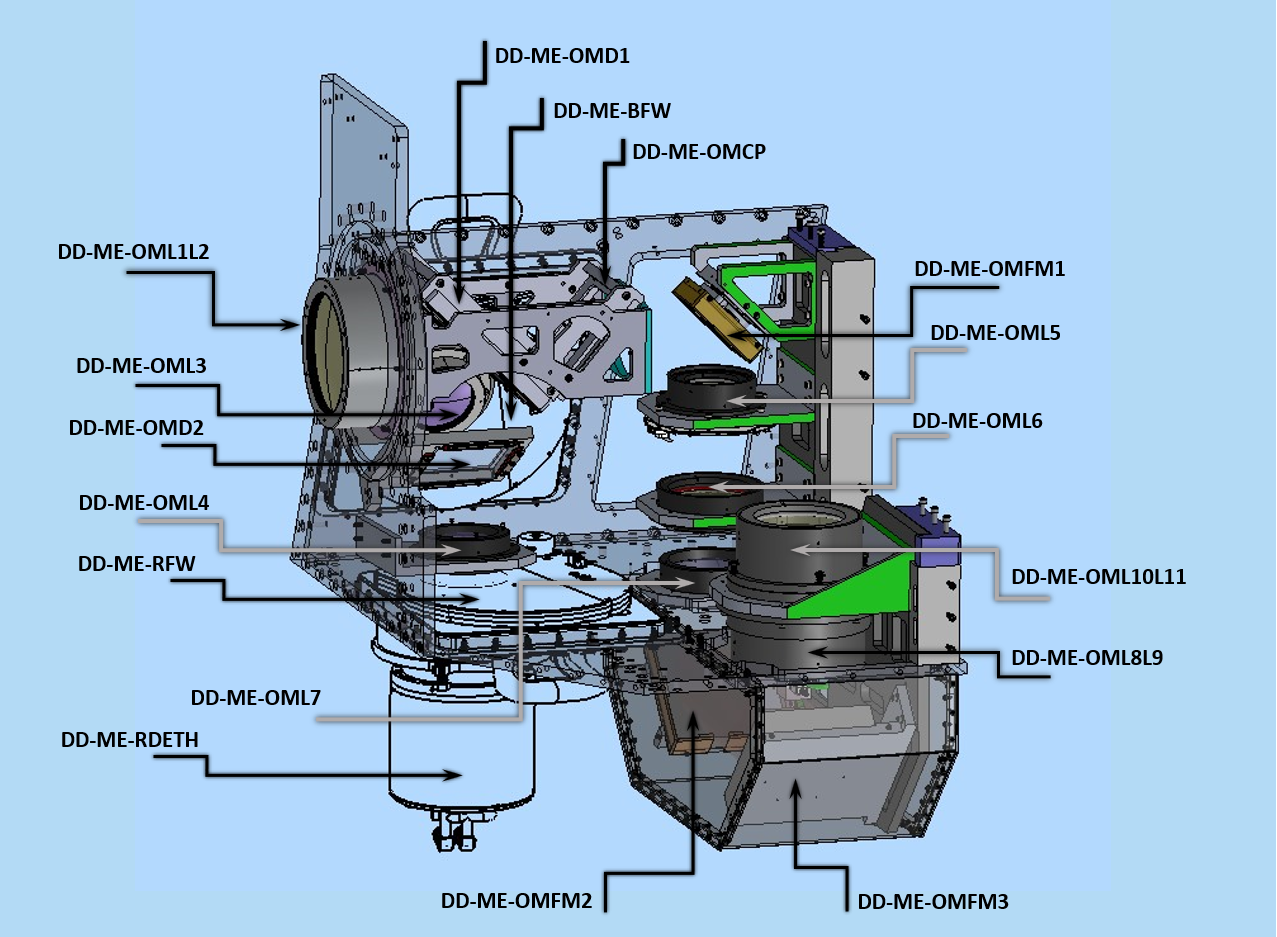
\includegraphics[width=\linewidth]{figures/OPTOMECH_LAYOUT_w_labels.png}
\end{center}
\caption{DDRAGO and WOB optomechanical layout.}
\label{figure:rosalia-DD_and_WOB}
\end{figure}

\section{Manufacturing Process and Materials}

All barrels and optomechanical parts will be manufactured from a special aluminium alloy of the 7000-series (Alumold${}^\circledR $ 500) and black finished. This material has been chosen for its ease of precision machining and excellent mechanical properties.

The main processes involved include turning, milling, drilling, routing and CNC machining. 

After machining, each component will be measured before assembly to verify that they comply with the requirements. To accomplish this task, we use the Mitutoyo Coordinate Measuring Machine at the Metrology Laboratory of the IAUNAM.
Other materials will be used according to their function and properties. Details will be given in the pertinent section.

\section{Reference Surfaces}

Each barrel will have a flange for fastening to their corresponding structural bracket or plate. The flanges, as well as their corresponding structural counterparts, will provide reference surfaces to locate the barrels in the correct position in the optical arrangement.

Inside each barrel there is another reference surface to keep the lens in its correct position inside the barrel. The inner profile of the barrels will make a tangential contact with the lenses convex surfaces or with flat bevels of concave surfaces, in order to reduce the mechanical stress on the lenses. In some cases, precision aluminium spacers are used to separate lenses in a same barrel. See Figure \ref{figure:Refsurfaces}

\begin{figure}
\begin{center}
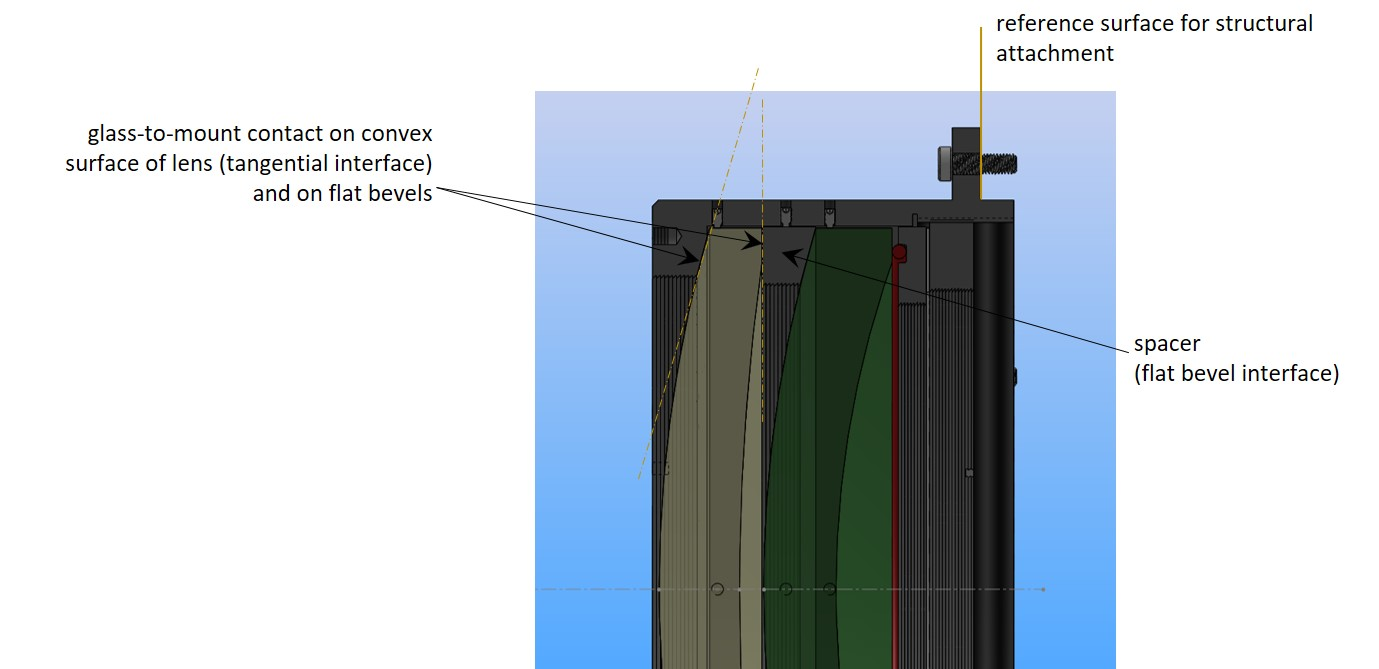
\includegraphics[width=0.7\linewidth]{figures/Reference-surfaces.jpg}
\end{center}
\caption{Reference surfaces of a barrel.}
\label{figure:Refsurfaces}
\end{figure}


\section{Glass-to-mount contact}

The glass-to-mount contact occurs on the polished surfaces of the lens or the bevel, so edging errors are not critical. The barrels are specified with a nominal clearance of 1 mm in diameter. The manufacturing tolerances on the lens diameters are $D^{+0} _{-0.05}$ mm and on the barrel inner diameters are $D^{+0.05} _{-0}$ mm.

\section{Centring of lenses}
 
Barrels include sets of radially directed nylon-tipped set-screws as an aid to center each lens and spacer during assembly. The centring screws are located in the same plane as the center of gravity of each element (see Figure \ref{figure:rosalia-set-screws}).

To verify the alignment of the lenses inside their barrels we will use the ALBATROS alignment system of the IAUNAM.

\begin{figure}
\begin{center}
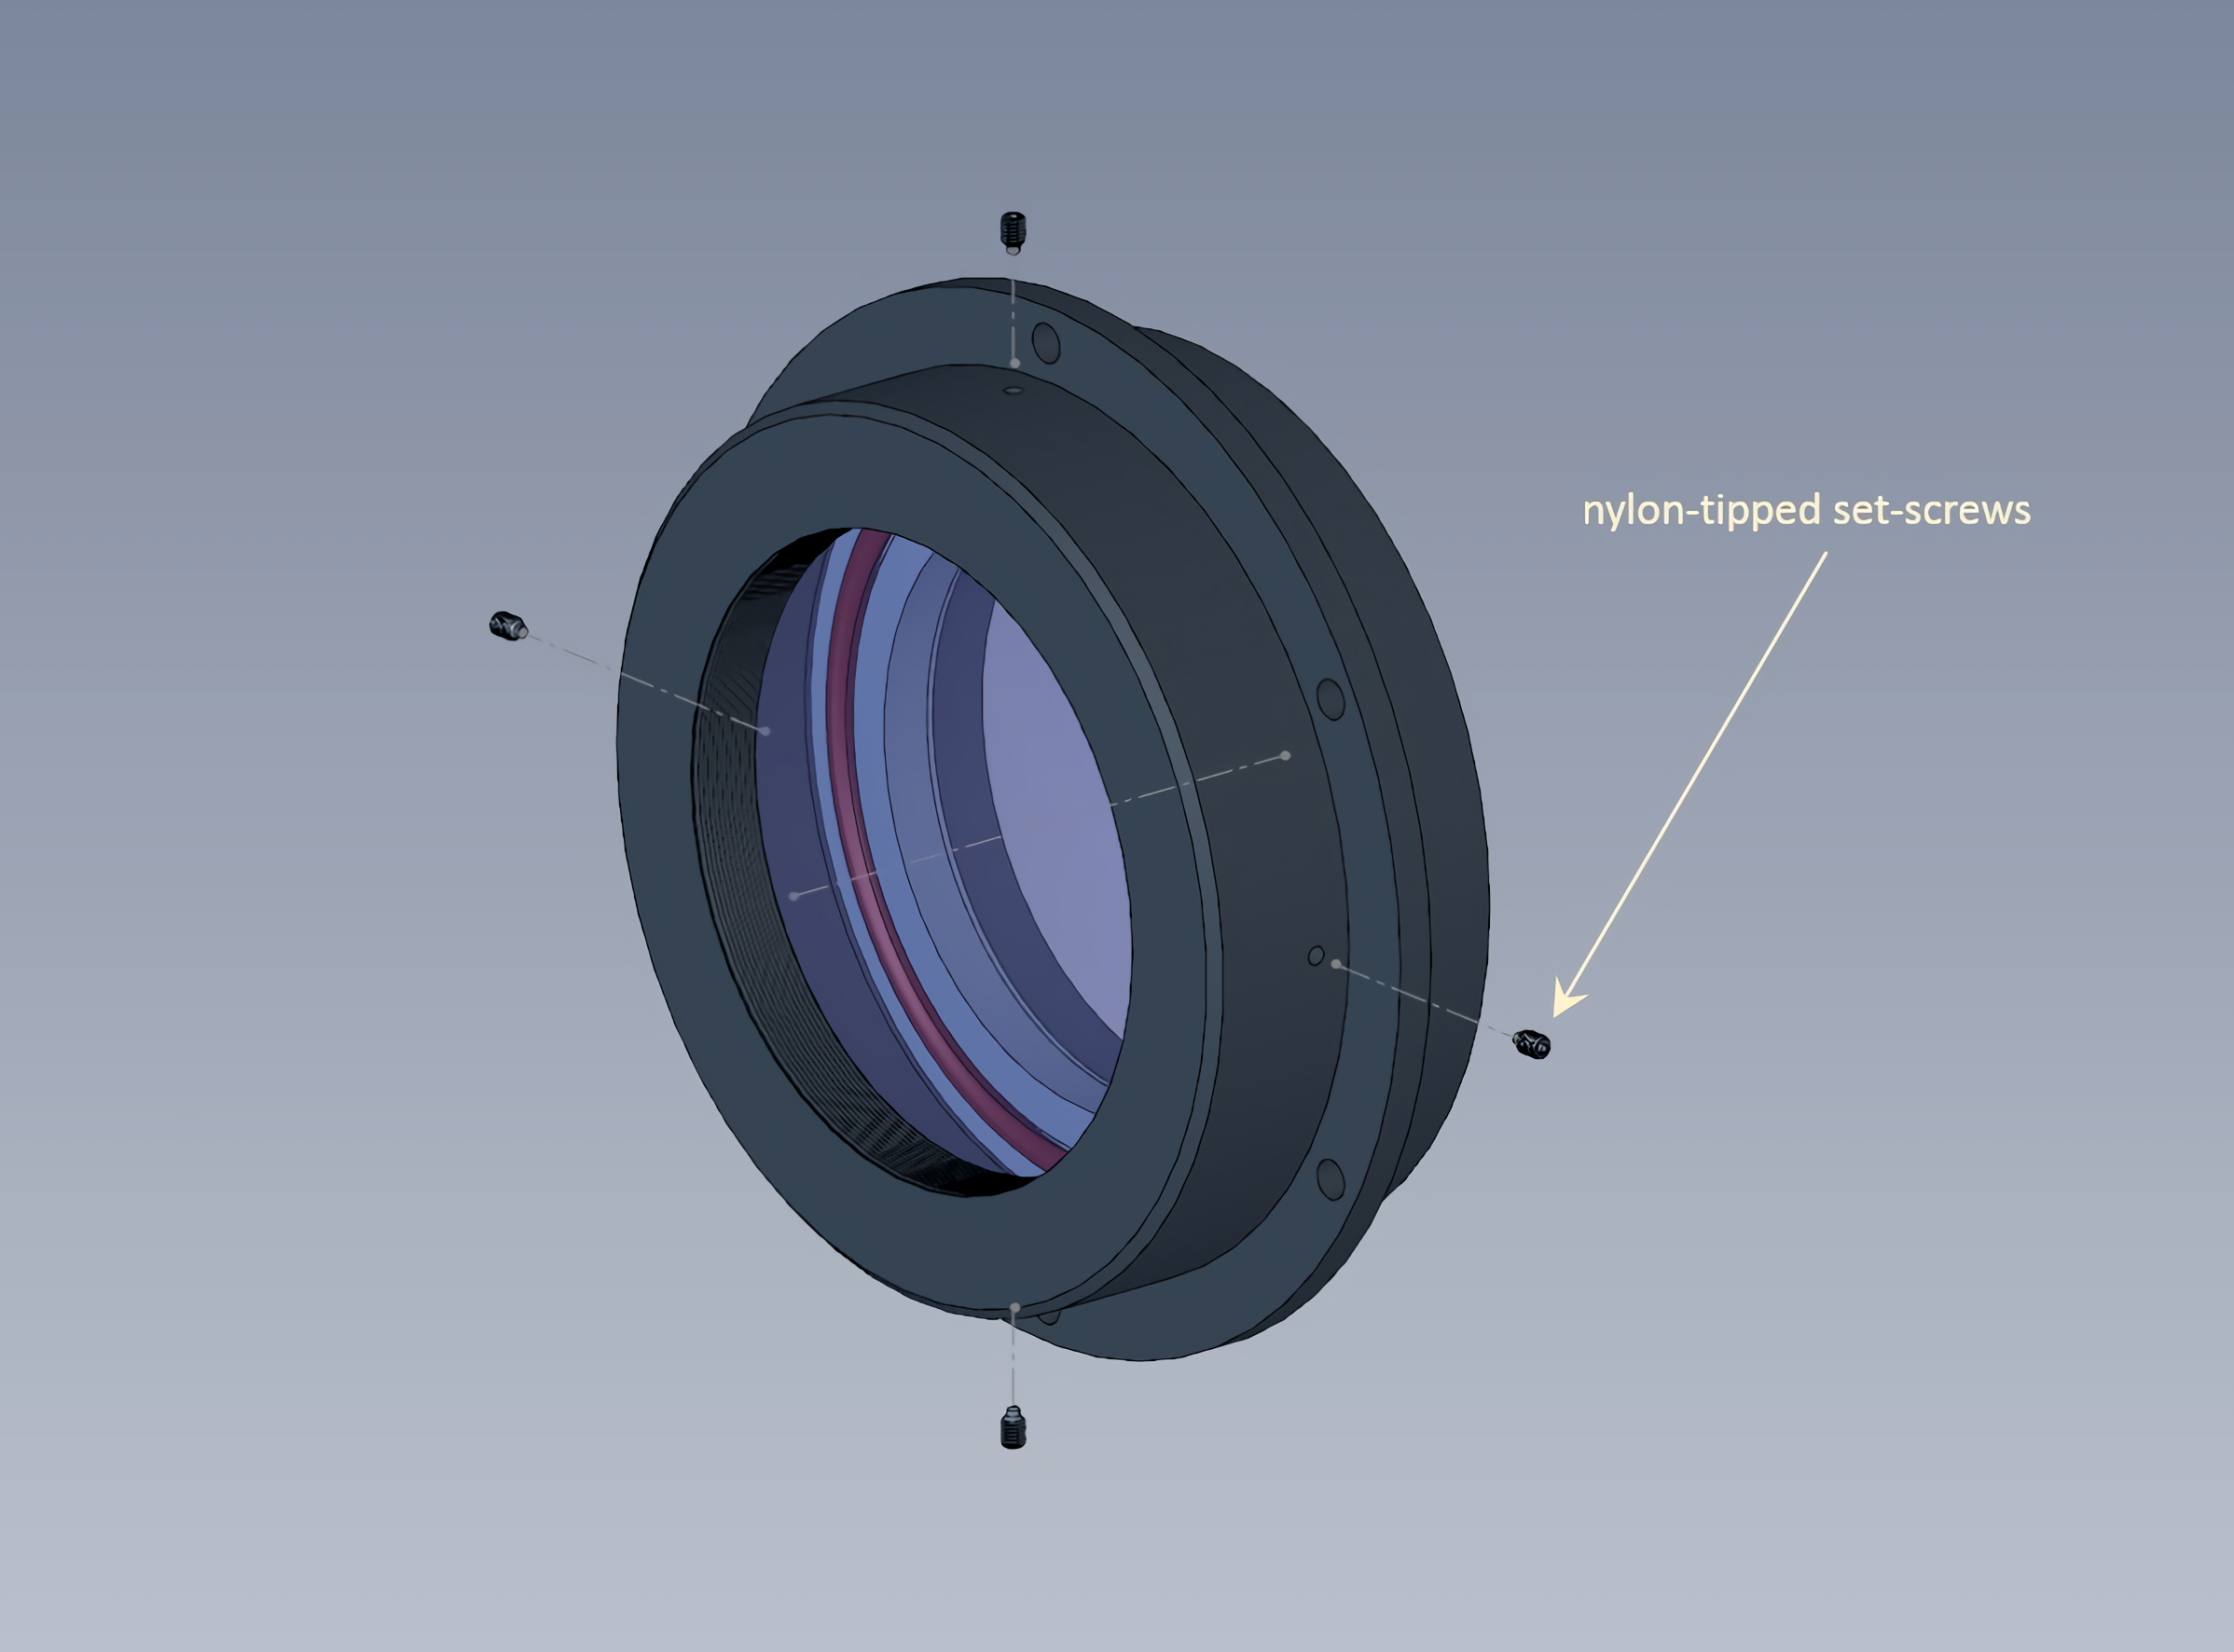
\includegraphics[width=0.7\linewidth]{figures/rosalia-set-screws.png}
\end{center}
\caption{Set-Screws for Centering.}
\label{figure:rosalia-set-screws}
\end{figure}

\section{Assembly preload}

After centring, an axial pre-load force will be applied to hold the lenses in their proper positions. The assembly preload is calculated considering lens materials, dimensions, geometry of the interfaces, tension and compression stresses and temperature conditions.

The pre-load will inevitably induce stress in the lenses. To reduce this to an acceptable level, the force should be distributed over a suitably large area of the lenses. Therefore, for the convex surfaces of the lenses we use tangential interfaces rather than corner interfaces. In the case of meniscus lenses, the concave surfaces cannot directly use tangential interfaces. Instead, these will have flat bevels ground into the circumference of their convex sides and we will use simple parallel interfaces.

The calculated axial preload is applied through a threaded preload ring using a specifically designed preload bench with an adapted torquemeter.

Since changes in temperature will result in changing preloads, this must be somehow compensated to avoid excessive stresses on lenses.

\section{Passive thermal compensation}

A thermal compensator was designed using a suitable elastomer which will help to compensate dimensional and preload variations due to temperature changes at optomechanical interfaces.

The rate of change of preload with temperature has been considered by calculating the temperature sensitivity factor for each configuration.

\begin{figure}
\begin{center}
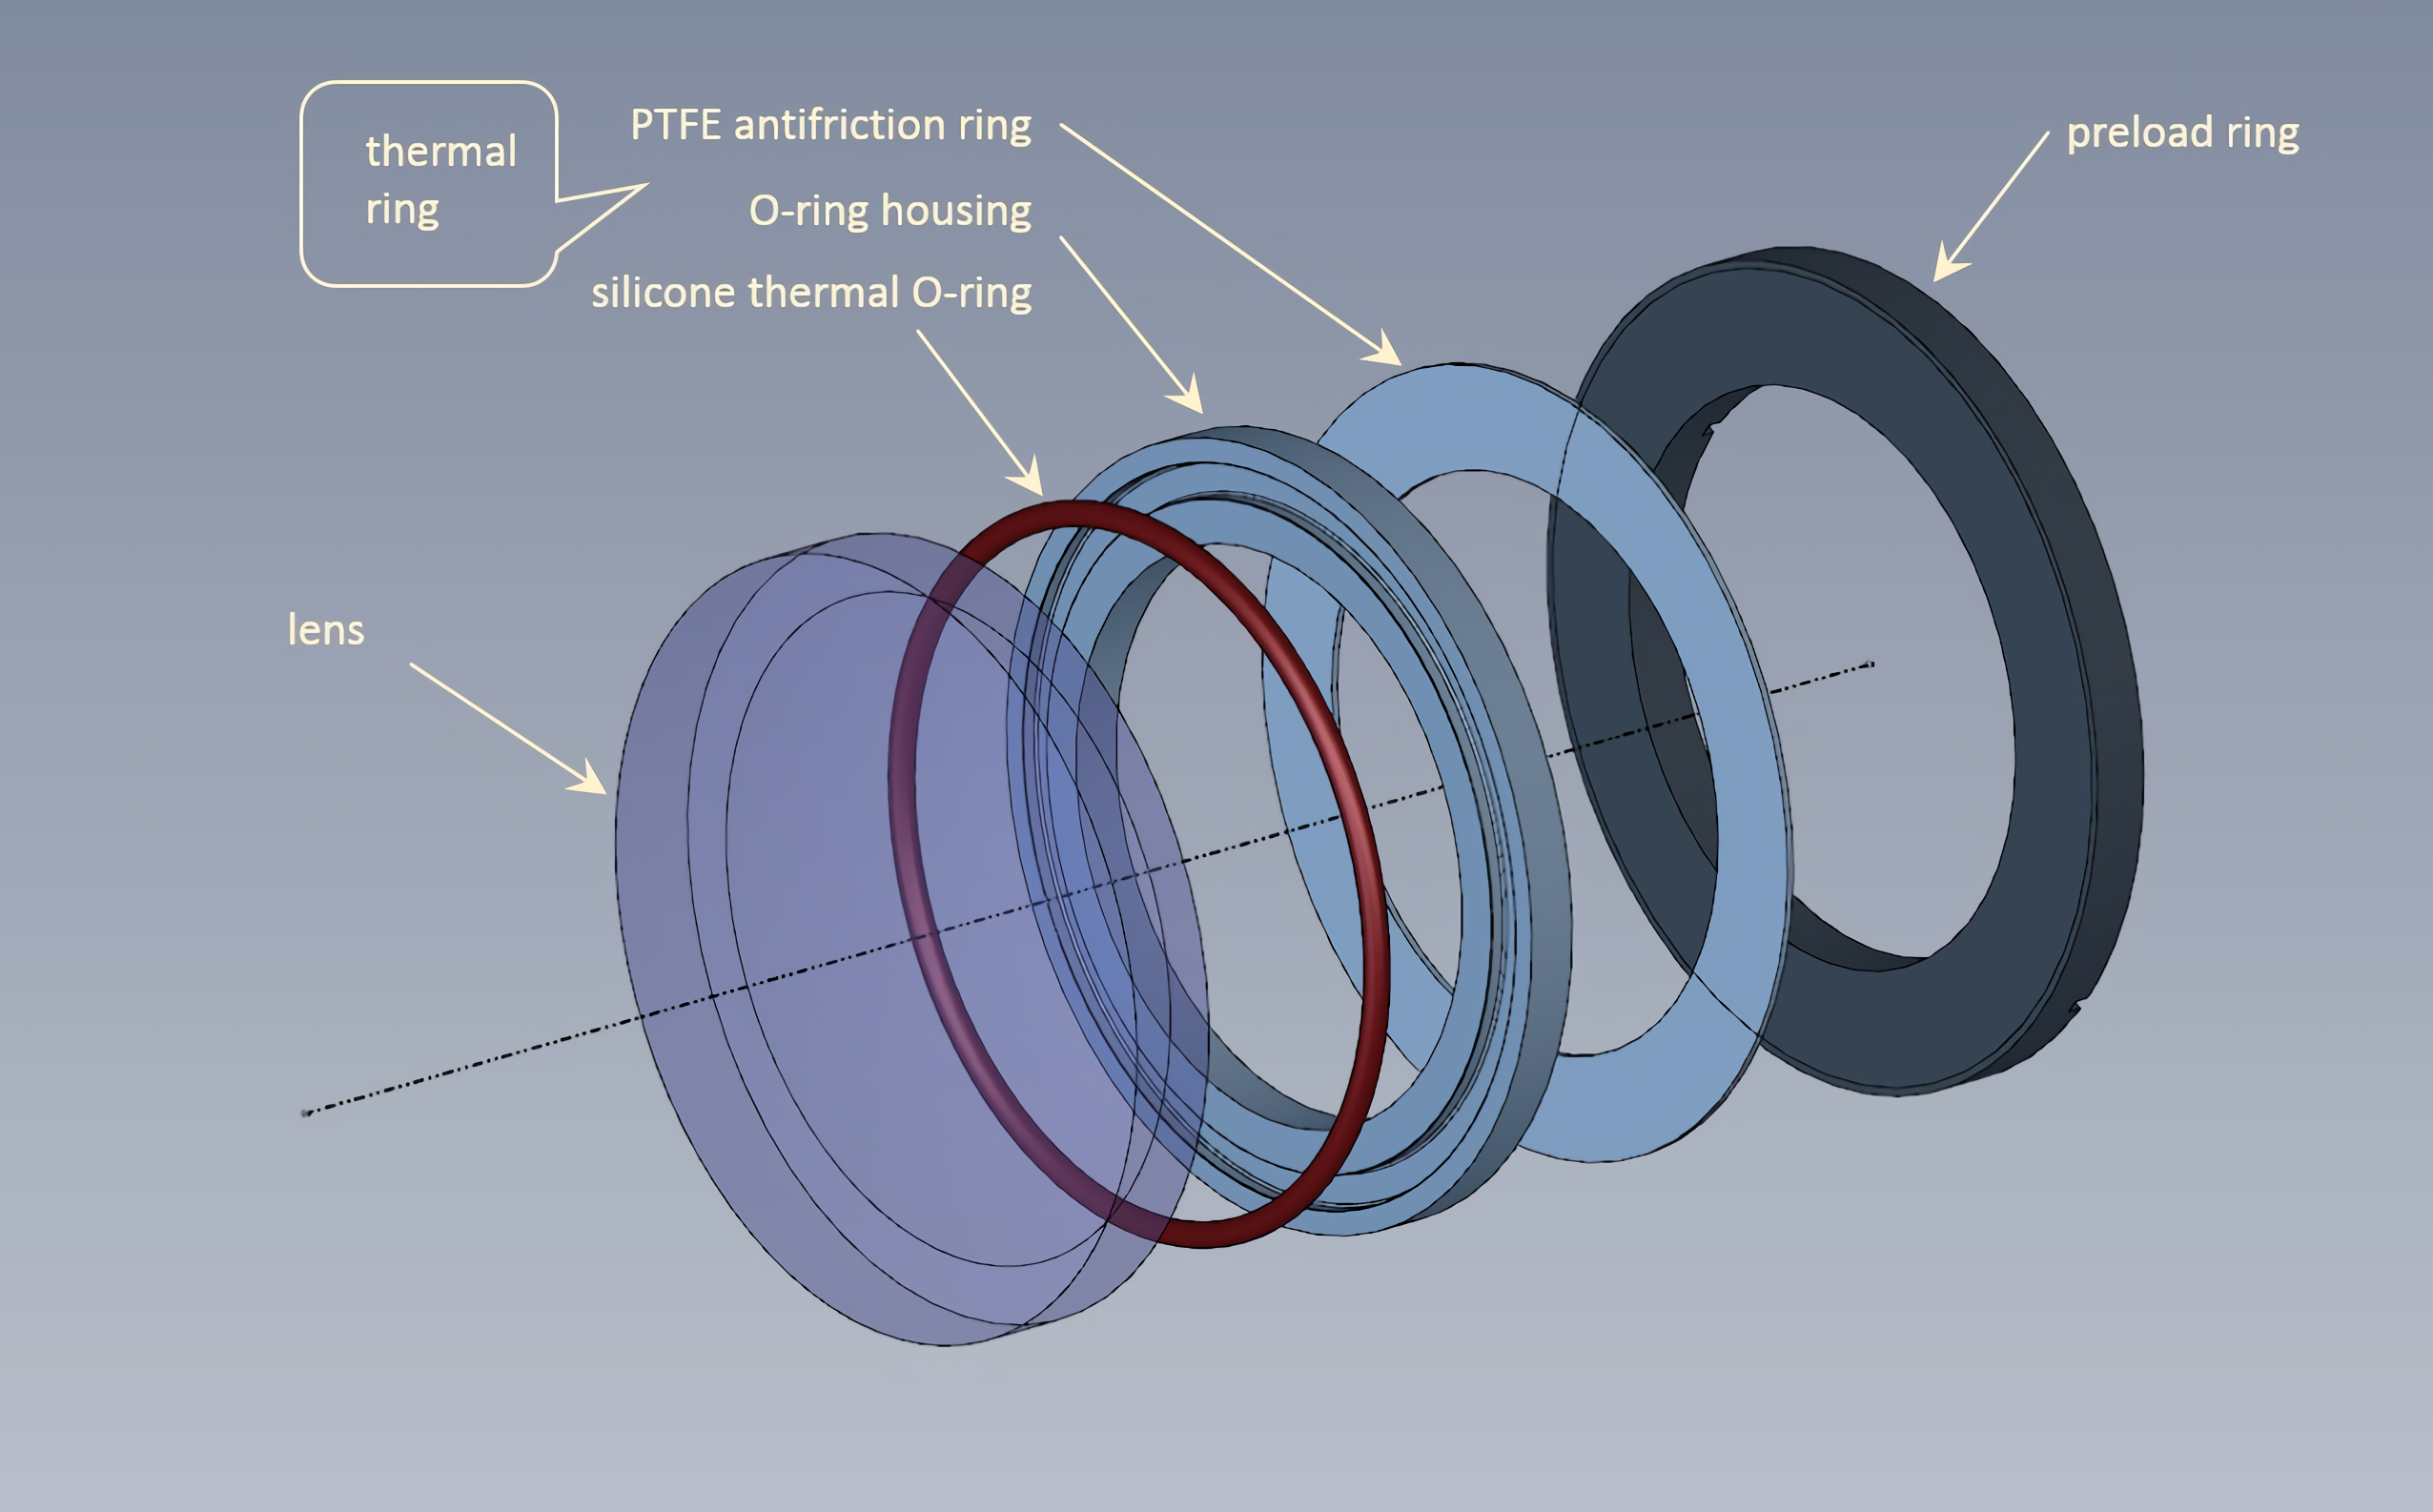
\includegraphics[width=0.7\linewidth]{figures/rosalia-rings.png}
\end{center}
\caption{The Pre-Load Mechanism.}
\label{figure:rosalia-rings}
\end{figure}

The pre-load is applied – and compensated thermally – by four mechanical components which are shown schematically in Figure \ref{figure:rosalia-rings}. First, there is an elastomeric O-ring that contacts a flat bevel ground into the concave surface of the last lens. Next, there is an aluminum O-ring holder to support the O-ring. Then there is a thin PTFE (Teflon) friction-reducing ring cut from 0.8 mm (actually 1/32 inch), glued to the O-ring holder. Finally, there is a threaded aluminum pre-load ring.


At assembly, the applied preload would compress the elastomeric O-rings, so we made tests to determine the relation between compression and load using a Shimadzu compression testing machine.

In the next section we will discuss about DDRAGO optomechanics and, in another section, about the WOB of CAGIRE.


%Here we describe the optomechanical design proposed for the three lens mounts for the DDRAGO lens groups, the common doublet L1+L2 (DR-ME-OML1L2 in the product tree), the blue channel field singlet L3 (DR-ME-OML3), and the red channel field singlet L4 (DR-ME-OML4), and for the DDRAGO plates, the D1 and D2 dichroics and the CP corrector plate.

%In the version 1.0 of this document, prepared for the PDR, we also presented a design for the L8+L9+L10 triplet from CAGIRE. The CAGIRE optomechanical supports have not been updated to use the new thermal compensator concept. Therefore, to avoid confusion, in this version we have omitted this and the other CAGIRE WOB lens mounts. (The optomechanical support for L11 is part of the cryostat work package being carried out by IRAP.)

%We begin by summarizing the design considerations. We then present the designs, first in a general sense and then individually for DR-ME-OML1L2, DR-ME-OML3, and DR-ME-OML4. We then discuss the required pre-load, the thermal compensation, and the likelihood of failure due to stresses. (Birefringence is discussed in \ref{optics}.)

%In terms of the lens barrels, the major change in the design from PDR is that we have changed the thermal compensator. In PDR, we proposed to use PTFE (Teflon) rings as the principal thermal compensator. However, as we developed this design we worried that precision PTFE rings, especially conical ones, would be difficult to manufacture. Therefore, we have now adopted silicone and EPDM O-rings as the thermal compensator. (Simple PTFE rings are used to avoid friction between the aluminium O-ring holder and the aluminium pre-load ring, but they no longer require machining in thickness.)

\chapter{DDRAGO Lens Optomechanical Design}

\begin{figure}
\begin{center}
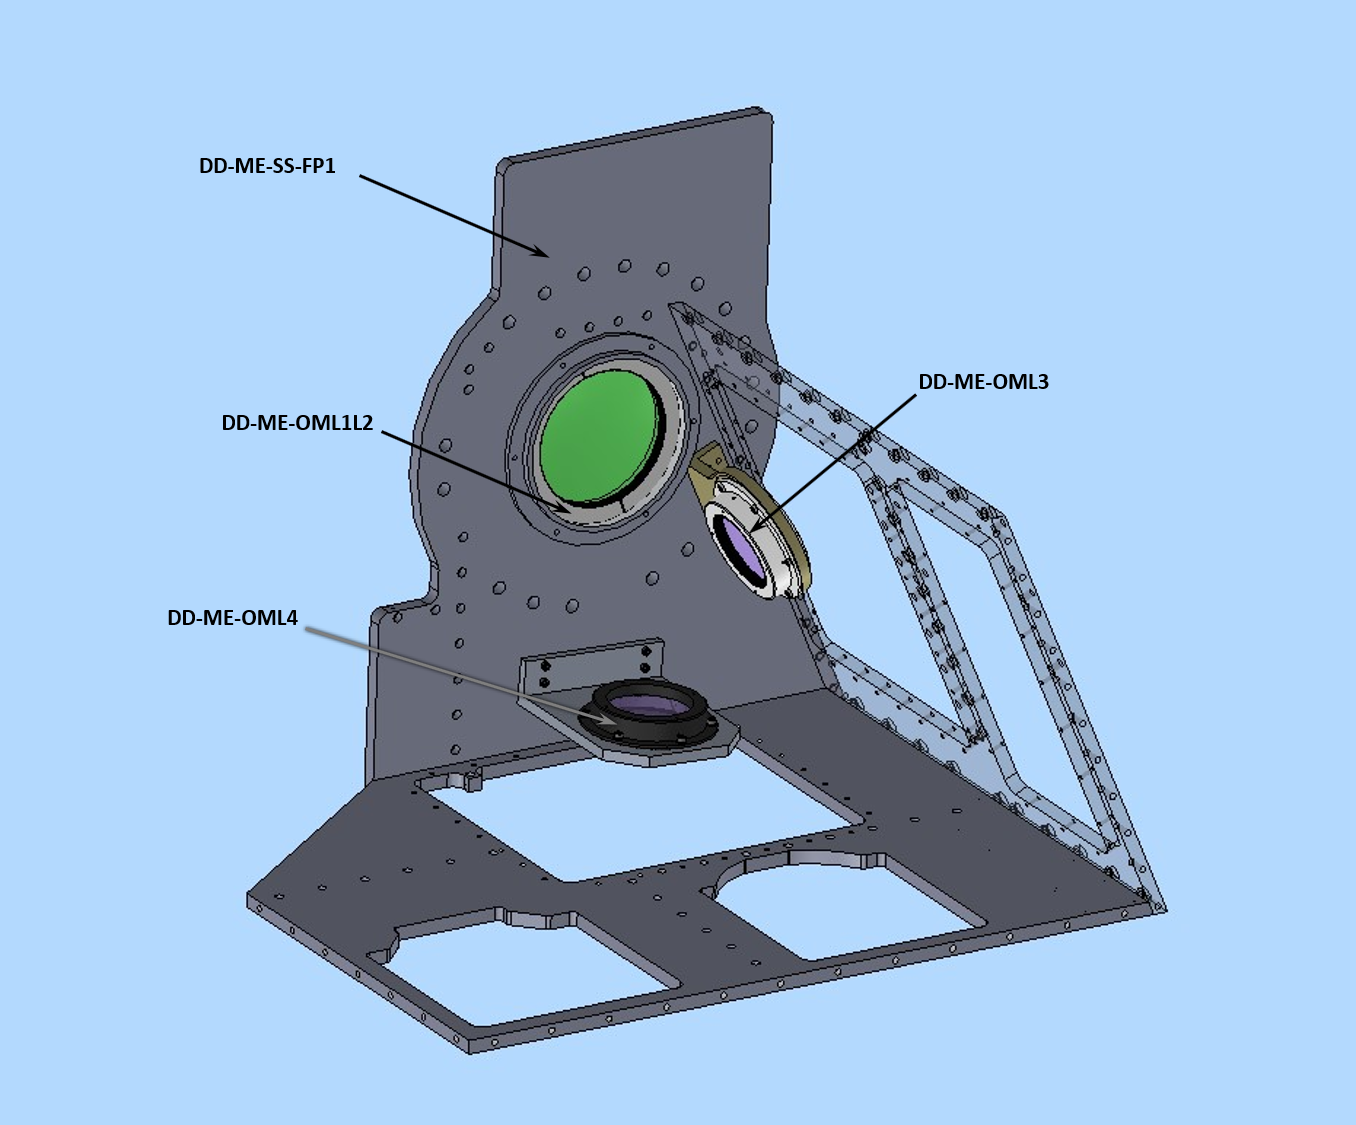
\includegraphics[width=0.7\linewidth]{figures/DDRAGO_OPTOMECH_LAYOUT_w_labels.png}
\end{center}
\caption{Optomechanical layout of DDRAGO lenses (L1L2, L3, L4).}
\label{figure:rosalia-DDRAGO-OPTOMECH}
\end{figure}

Here we describe the optomechanical design proposed for the three lens mounts of the DDRAGO lens groups, the common doublet L1+L2 (DD-ME-OML1L2 in the product tree), the blue channel field singlet L3 (DD-ME-OML3), and the red channel field singlet L4 (DD-ME-OML4). In Figure \ref{figure:rosalia-DDRAGO-OPTOMECH}, the layout of these optomechanical components is shown mounted on the structure.

The DDRAGO plates D1 and D2 dichroics and the CP corrector plate will be described in the next section (Section 6).

We begin by summarizing the design considerations and the general design, then we present the individual designs for DD-ME-OML1L2, DD-ME-OML3, and DD-ME-OML4. We then discuss the corresponding tolerances, the centering method, the required preload and thermal compensation, manufacturing processes, and the likelihood of failure due to stresses. (Birefringence is discussed in \ref{optics}.)


\section{Considerations and General Design}

The DDRAGO optomechanical design presented here was developed according to the following specifications established by the optical design:

\begin{figure}
\begin{center}
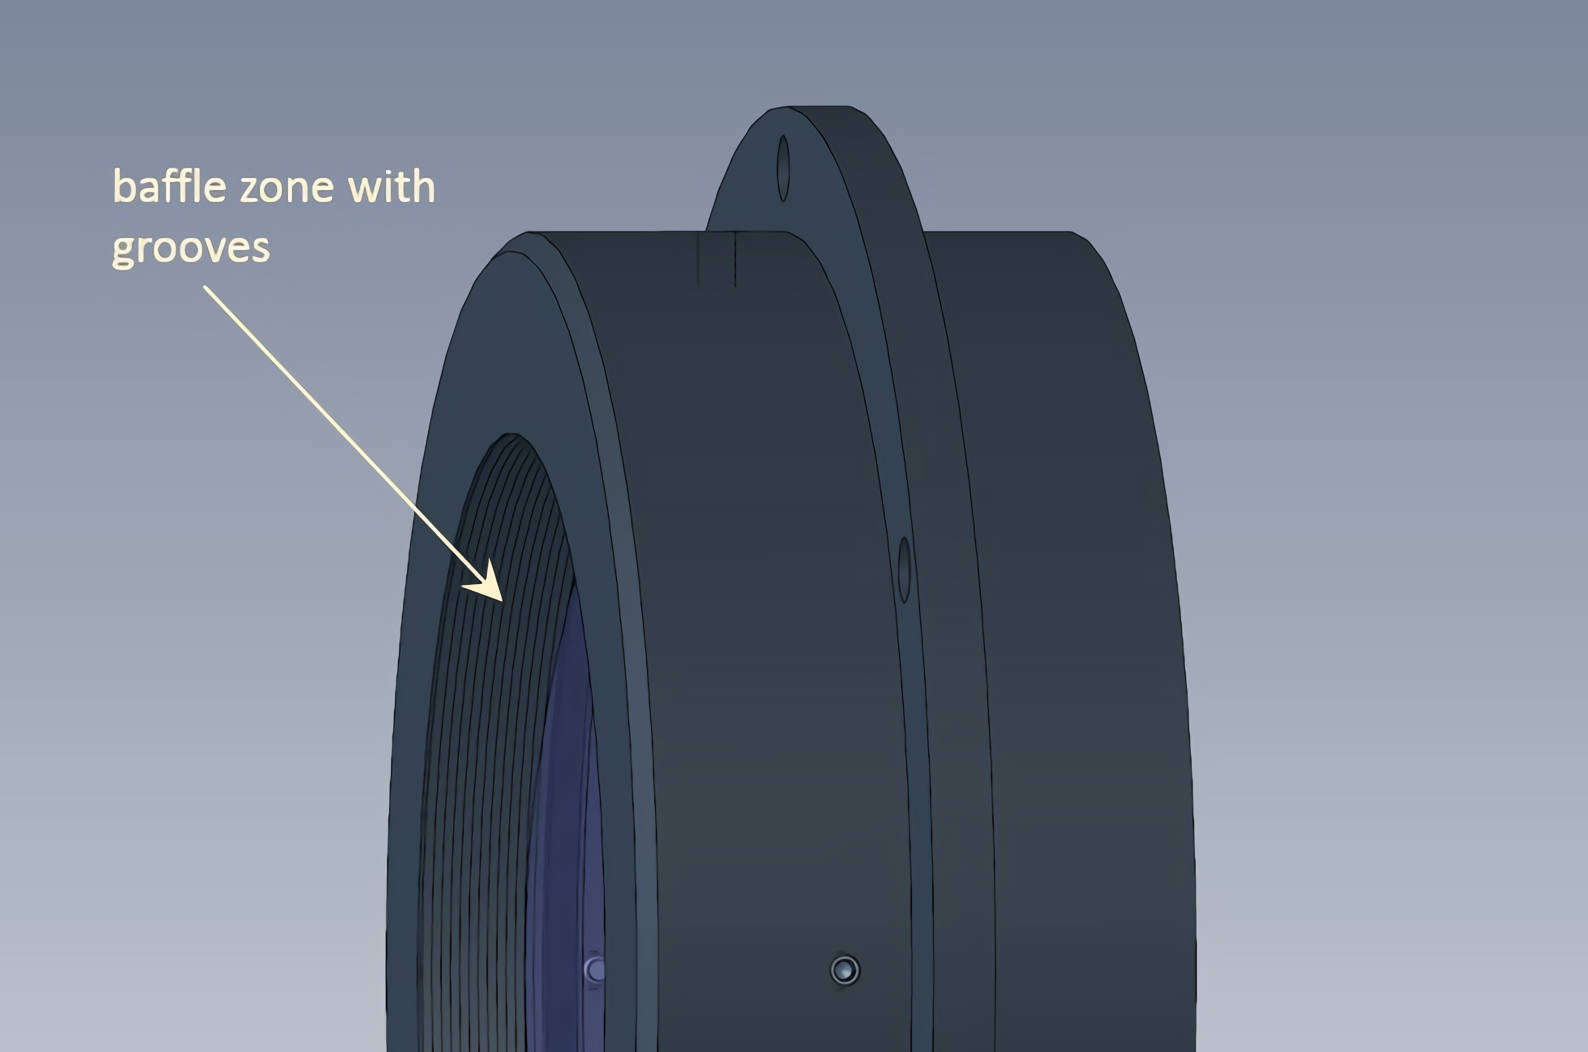
\includegraphics[width=0.7\linewidth]{figures/rosalia-grooves.png}
\end{center}
\caption{Grooves to Reduce Scattered Light.}
\label{figure:rosalia-grooves}
\end{figure}

\begin{enumerate}
\item All of the DDRAGO optics will be mounted on the same structural plate (DD-ME-SS-FP1), the plate that attaches to COLIBRÍ derotator flange. This will allow us to integrate the optics on the plate, then perform metrology, and finally integrate the plate into the support structure. (This was suggested by our colleagues at LAM in the previous informal review.)
\item The lens materials are Ca$F_2$, N-BaK4, and Fused Silica.
3. The barrels should provide an attachment flange to allow them to be fixed to the plates of the support structure (L1+L2) or to precision L-brackets (L3 and L4).
\item The inner diameter at the entrance of each barrel will have an appropriate dimension so to act as a baffle. Furthermore, the inner surfaces of the barrel and aluminium rings will be grooved with a 60 deg pattern and 800 microns height (see Figure \ref{figure:rosalia-grooves}).
\item The tolerances in axial positioning, decentering, and tilts are given by the optical design.
\item The alignment and verification of lenses inside their respective barrels will be carried out with the IA-UNAM aligning system ALBATROS.
\item The calculated preload on lenses in their barrels will be applied in a controlled and measured manner 
\item Mechanical parts and lenses will be manufactured and integrated at a temperature of about 20 C
\item The operational temperature range is -15 C to 20 C.
\item The survival temperatures is from -25 C to 50 C.
\item The optomechanical design must protect the lenses and maintain their alignment against accelerations of $5g$. (The requirement is that the instruments must survive accelerations of $10g$ during transport, but we assume that the packing will reduce an external $10g$ acceleration sufficiently that a maximum of $5g$ will be imparted to the instrument.)
\item The optics will be protected with covers for protection during handling and transport. These will consist of microfiber bags covering the optomechanics and acrylic plates fixed to the structure where necessary.
\end{enumerate}

Table \ref{table:lens-barrel-product-tree} shows an extract of DDRAGO Product Tree table relevant for the lenses supports.

\begin{table}
\caption{Extract of the Product Tree Table Relevant for the Lens Mounts L1 to L4}
\label{table:lens-barrel-product-tree}
\begin{center}
\small
\begin{tabular}{ll}
\hline
\hline
Code                &Description\\
\hline
DD-ME-OML1L2        &Optomechanics for L1 and L2\\
DD-ME-OML1L2-BAR    &Barrel\\
DD-OP-L1            &Lens L1\\
DD-ME-OML1L2-SPA		&Spacer\\
DD-OP-L2            &Lens L2\\
DD-ME-OML1L2-OR		  &O-Ring (EPDM)\\
DD-ME-OML1L2-ORH		&O-Ring Holder\\
DD-ME-OML1L2-FRR		&Friction-Reducing Ring (PTFE)\\
DD-ME-OML1L2-PLR		&Pre-Load Ring\\
DD-ME-OML1L2-CSS		&Centering Set-Screw\\
\hline
DD-ME-OML3          &Optomechanics for L3\\
DD-ME-OM3-LBR       &L-Bracket\\
DD-ME-OM3-BAR       &Barrel\\
DD-OP-L3            &Lens L3\\
DD-ME-OML3-OR		    &O-Ring (Silicone)\\
DD-ME-OML3-ORH	  	&O-Ring Holder\\
DD-ME-OML3-FRR	  	&Friction-Reducing Ring (PTFE)\\
DD-ME-OML3-PLR	  	&Pre-Load Ring\\
DD-ME-OML3-CSS	  	&Centering Set-Screw\\
\hline
DD-ME-OML4          &Optomechanics for L4\\
DD-ME-OM4-LBR       &L-Bracket\\
DD-ME-OM4-BAR       &Barrel\\
DD-OP-L4            &Lens L4\\
DD-ME-OML4-OR	   	  &O-Ring (Silicone)\\
DD-ME-OML4-ORH  		&O-Ring Holder\\
DD-ME-OML4-FRR  		&Friction-Reducing Ring (PTFE)\\
DD-ME-OML4-PLR  		&Pre-Load Ring\\
DD-ME-OML4-CSS	  	&Centering Set-Screw\\
\hline
\end{tabular}
\end{center}
\end{table}

Table \ref{table:physical-properties} gives the physical properties of the materials used in DDRAGO: the thermal expansion coefficient $\alpha$, the Poisson ratio $\nu$, the modulus of elasticity $E$, and density $\rho$.

\begin{table}
\caption{Physical Properties of Materials}
\label{table:physical-properties}
\begin{center}
\small
\begin{tabular}{lccccl}
\hline
\hline
Material&
$\alpha$&
$\nu$&
$E$&
$\rho$&
Reference\\
&
\unit{C^{-1}}&
&
Pa&
\unit{g\,cm^{-3}}&
\\
\hline
\CaF&
$1.885 \times 10^{-5}$&
0.26&
$7.580 \times 10^{10}$&
3.18\phantom{0}&
oharacorp.com\\
N-BaK4&
$7.000 \times 10^{-6}$&
0.24&
$7.700 \times 10^{10}$&
3.05\phantom{0}&
schott.com\\
Fused Silica&
$5.000 \times 10^{-7}$&
0.16&
$7.270 \times 10^{10}$&
2.201&
corning.com\\
Alumold${}^\circledR$ 500&
$2.37\phantom{0} \times 10^{-5}$&
0.33&
$7.20\phantom{0} \times 10^{10}$&
2.82\phantom{0}&
carrs-tool.co.uk\\
Silicone&
$1.80\phantom{0} \times 10^{-4}$&
0.5\phantom{0}&
$8.5\phantom{00} \times 10^{5\phantom{0}}$&
1.1\phantom{00}&
parker.com\\
EPDM&$1.602\times 10^{-4}$&$0.48$&$6.0\phantom{00}\times 10^{6\phantom{0}}$&$1.43\phantom{0}$& parker.com\\
PTFE&
$8.00\phantom{0} \times 10^{-5}$&
0.46&
$5.17\phantom{0} \times 10^{8\phantom{0}}$&
2.18\phantom{0}&
dmh.at\\
\hline
\end{tabular}
\end{center}
\end{table}

%The optomechanical design presented here was developed according to the following specifications established by the optical design:
%\begin{enumerate}
%\item
%All of the DDRAGO optics will be mounted on the same structural plate, the plate that attaches to the derotator flange. This will allow us to integrate the optics on the plate, then perform metrology, and finally integrate the plate into the support structure. (This was suggested by our colleagues at LAM in the previous informal review.)
%\item
%The lens materials are {\CaF}, N-BaK4, and fused silica.
%\item The barrels should provide an attachment flange to allow them to be attached to the plates of the support structure (L1+L2) or to precision L-brackets (L3 and L4).
%\item The tolerances in axial positioning, decentering, and tilts are given by the optical design.
%\item The alignment and verification of lenses inside their respective barrels will be carried out with the IA-UNAM aligning system ALBATROS.
%\item Mechanical parts and lenses will be manufactured and integrated at a temperature of about 20~C
%\item The operational temperature range is $-15$~C to 20~C.
%\item The survival temperatures is from $-25$~C to 50~C.
%\item The supports must protect the lenses and maintain their alignment against accelerations of $5g$. (The requirement is that the instruments must survive accelerations of $10g$ during transport, but we assume that the packing will reduce an external $10g$ acceleration sufficiently that only $5g$ will be imparted to the instrument.)
%\end{enumerate}

\section{The DD-ME-OML1L2 Optomechanical Design}

The group constitutes the common doublet for DDRAGO and CAGIRE and is situated in the structural plate that will contact the derotator flange.
L1+L2 is a doublet of meniscus lenses, L1 in Ca$F_2$ and L2 in N-BAK4, both with a diameter of 170 mm. The design of the barrel is shown in Figures \ref{figure:OML1L2-ID} and \ref{figure:OML1L2-CSV}.


\begin{figure}
\begin{center}
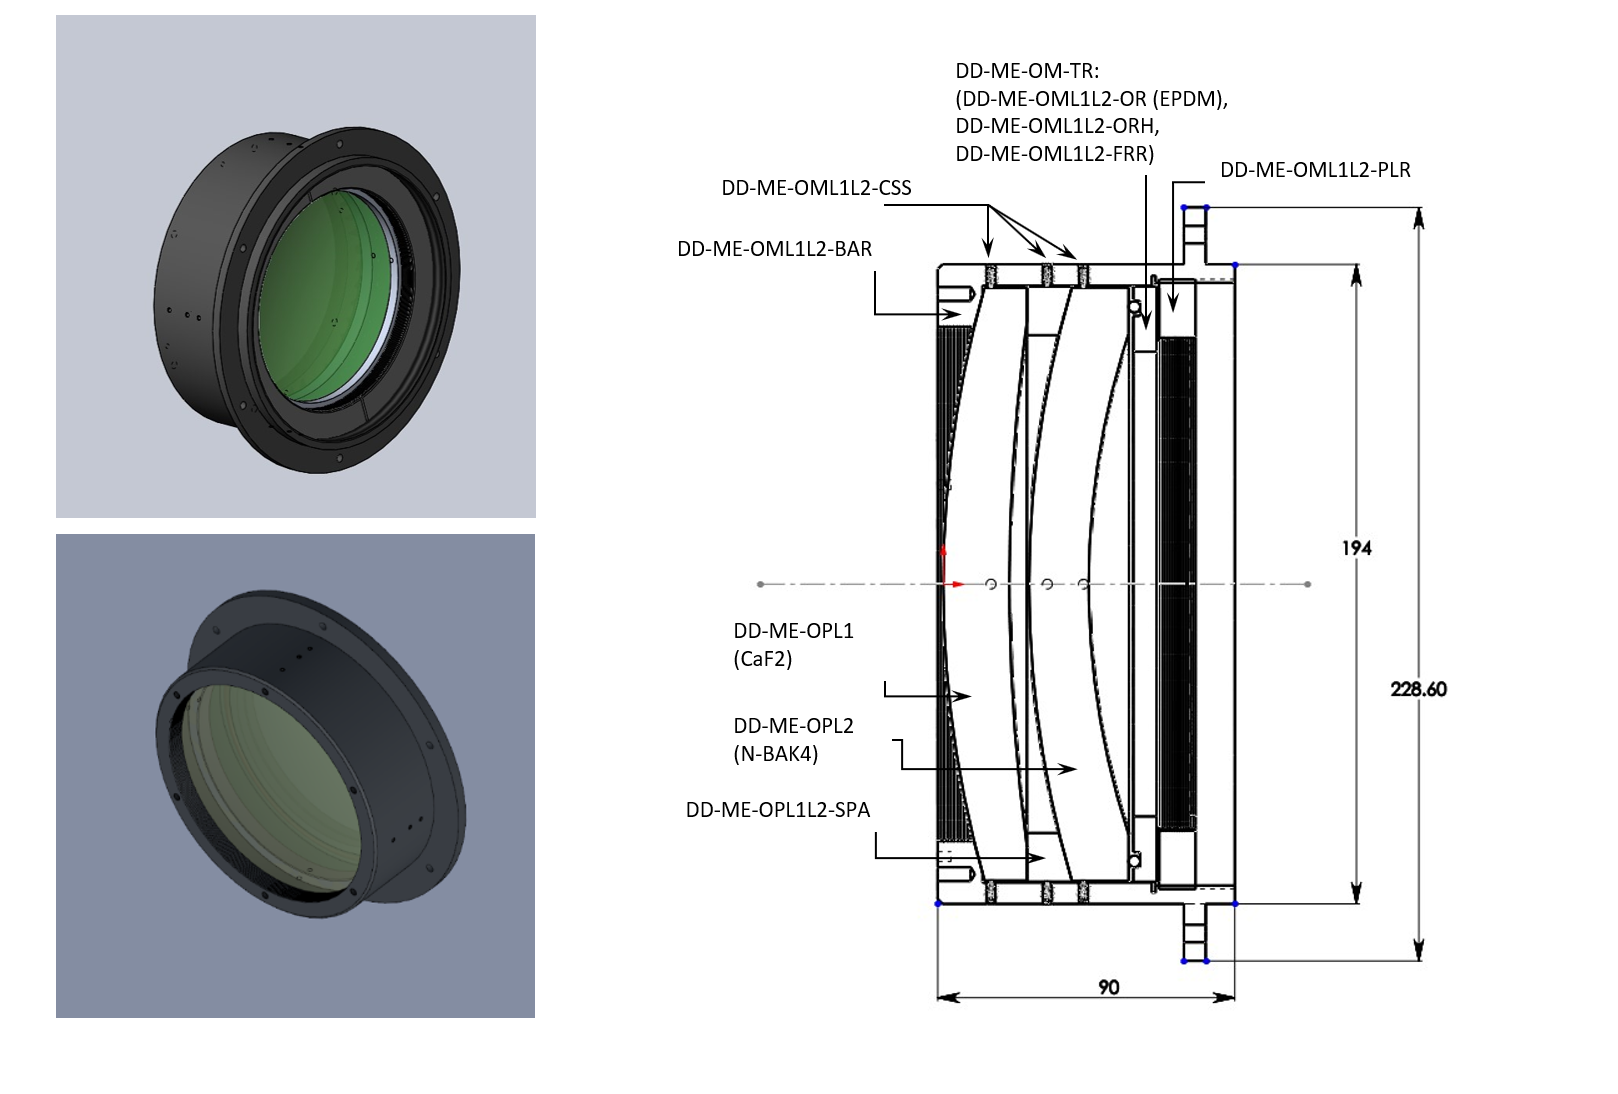
\includegraphics[width=1.1\linewidth]{figures/DD-ME-OML1L2-ID.png}
\end{center}
\caption{DD-ME-OML1L2 3d model (front and back views) and cross-section view of the Optomechanical Design.}
\label{figure:OML1L2-ID}
\end{figure}

\begin{figure}
\begin{center}
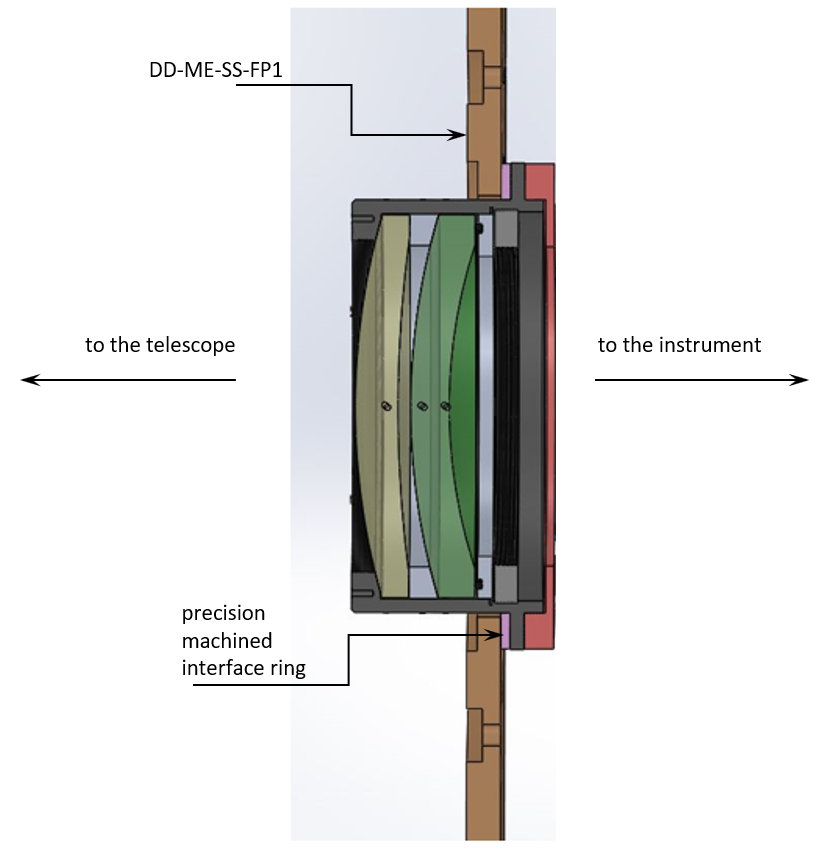
\includegraphics[width=0.7\linewidth]{figures/DD-ME-OML1L2_and_FP1.png}
\end{center}
\caption{Cross-section view of DD-ME-OML1L2 mounted on Structural Plate FP1 with Interface Ring.}
\label{figure:OML1L2-CSV}
\end{figure}


The first surface of L1 is convex and contacts a conical shoulder that is machined in the barrel and provides tangential support. Between L1 and L2 there is a precision Alumold${}^\circledR $ spacer contacting the flat bevel of lens L1 and the convex surface of L2. The exact thickness of this spacer was adjusted after metrology of lenses (see \ref{aiv}), and we obtained a precision of 15 microns, which is well within the 200 microns optical tolerance.

After L2 we have the thermal compensator that, in this case, uses an EPDM O-ring with a durometer of 70 Shore A and a section diameter of 3.5 mm (Parker${}^\circledR $ 2-259), since the properties of this material in combination with the properties of the lens and the aluminium led us to a convenient value of thermal sensitivity factor. 

The barrel has threaded holes for centring set-screws, giving x and y adjustments of L1, the spacer, and L2. These holes are in the planes of the center of gravity of each lens and the spacer in order to have a precise control of their positions.

The last element in the assembly is the preload ring by means of which the calculated preload is applied and the lenses are fixed in their specified place. The torque applied on the pre-load ring during assembly gave the required pre-load and compressed the O-ring by 27\%.

In the instrument, the flange of the barrel will be fixed to the inner surface of DD-ME-SS-FP1 (Plate 1) and its axial position will be adapted with a precision machined interface ring. 

When the instrument is mounted on the telescope, the barrel will extend into the derotator tunnel.

On its front surface, the barrel has a set of threaded holes to receive the mount for the spherical testing mirror STM (see Figure \ref{figure:alex-omstm}) when in verification process.

\begin{figure}
\begin{center}
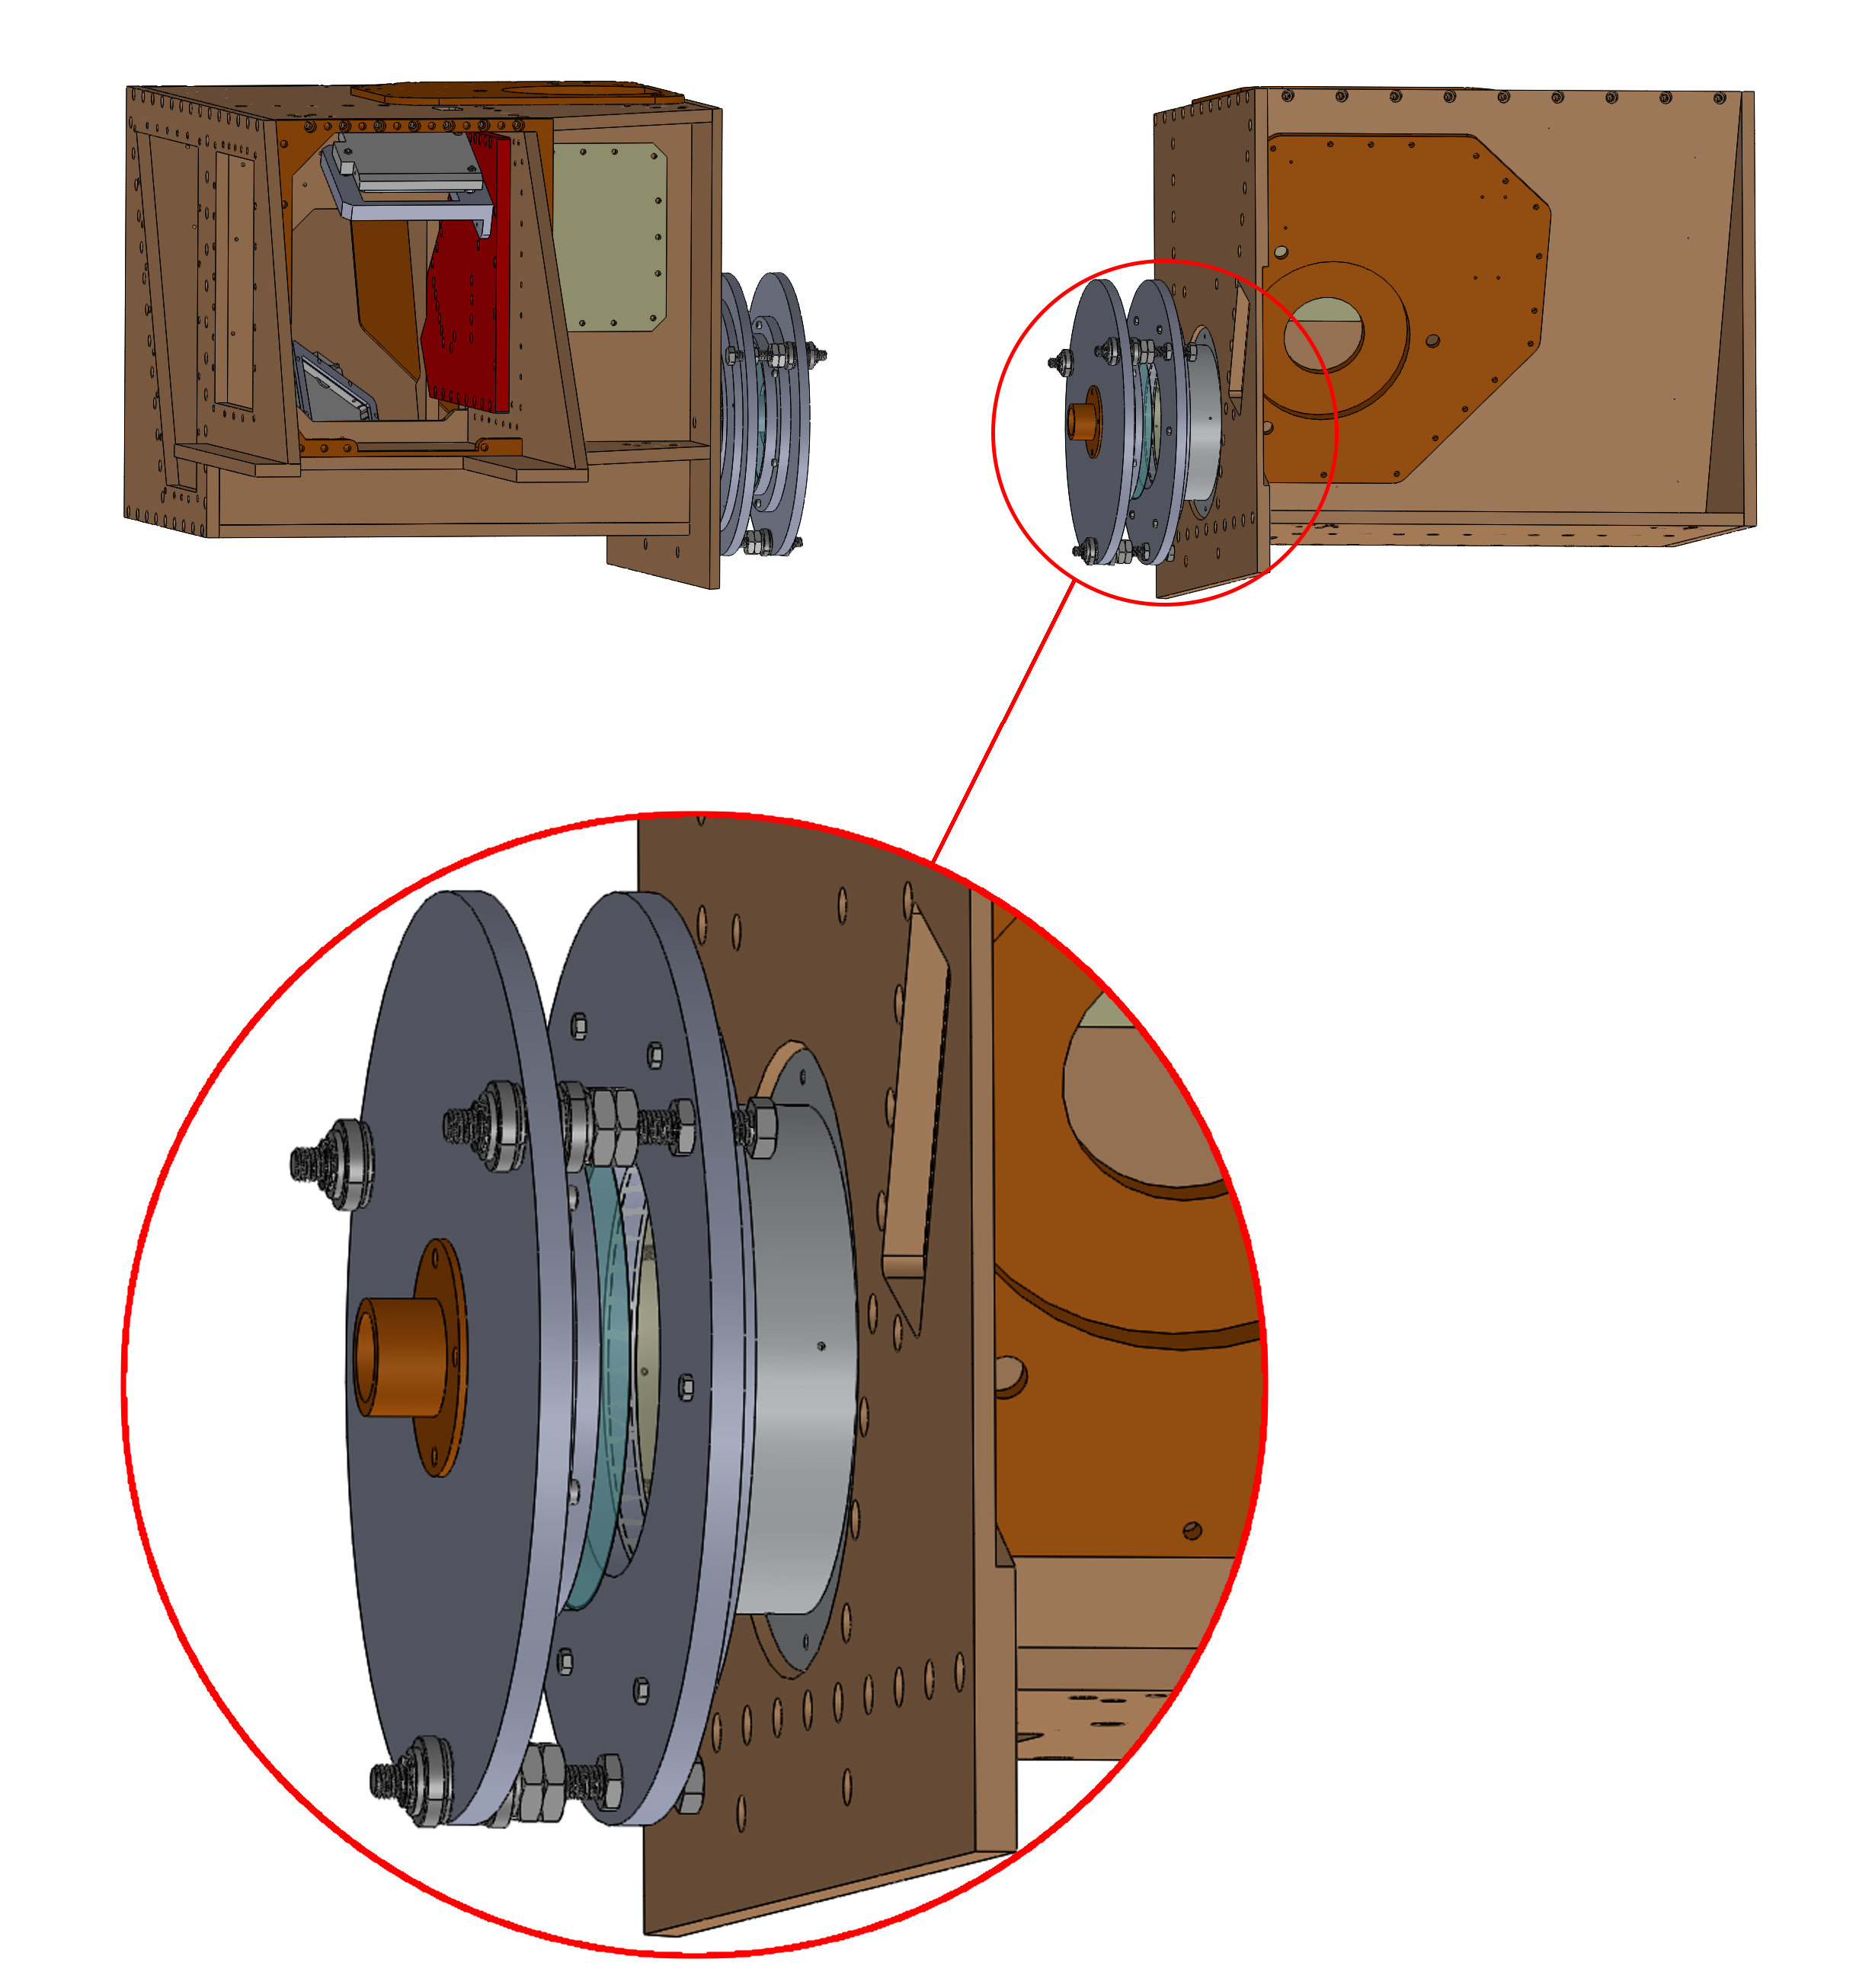
\includegraphics[width=0.7\linewidth]{figures/alex-omstm.jpg}
\end{center}
\caption{The DD-ME-OML1L2 Barrel with the STM Mounted}
\label{figure:alex-omstm}
\end{figure}

We will reuse the OML1L2 optomechanics from DDRAGUITO without modification in DDRAGO since it thoroughly satisfies the optical requirements. The precision we achieved in the centering of these lenses inside its barrel is of 20 microns with a relative tilt of less than 2 arcmin  (ref. Table \ref{table:tolerances}).

For handling and transport, the optics will be protected by a Nylamid ${}^\circledR $ made front cover attached with screws to the barrel.

\section{The DD-ME-OML3 Optomechanical Design}

As said in a previous section, we will reuse the OML3 barrel from DDRAGUITO that hosts the blue channel L3 field lens replacing the original lens with a new one. The only difference between the former and the latter is the size of the bevel: the new lens has a wider flat bevel which requires a slightly different O-ring holder and preload ring (OML3-ORH and OML3-PLR), but we can reuse the barrel (OML3-BAR).

L3 is a singlet meniscus lens in Fused Silica with a diameter of 108 mm. It constitutes the blue channel field lens. The design of the lens barrel is shown in Figures \ref{figure:OML3-ID} and \ref{figure:OML3-BR}. The first surface of L3 is convex and contacts with a conical shoulder that is machined in the barrel and provides tangential support. The second surface has a flat bevel in contact with its thermal ring. In this case, the chosen material for the O-ring is Silicone, the cross-section diameter of this O-ring is 3.5 mm (Parker${}^\circledR $ 2-240). The torque applied with its retaining ring during assembly will give the required pre-load and will compress the O-ring by 21\% at maximum compression.

The barrel has threaded holes for four centering set-screws, giving x and y adjustments of L3. These holes are in the planes of the center of gravity of the lens in order to have precise control of its position.

\begin{figure}
\begin{center}
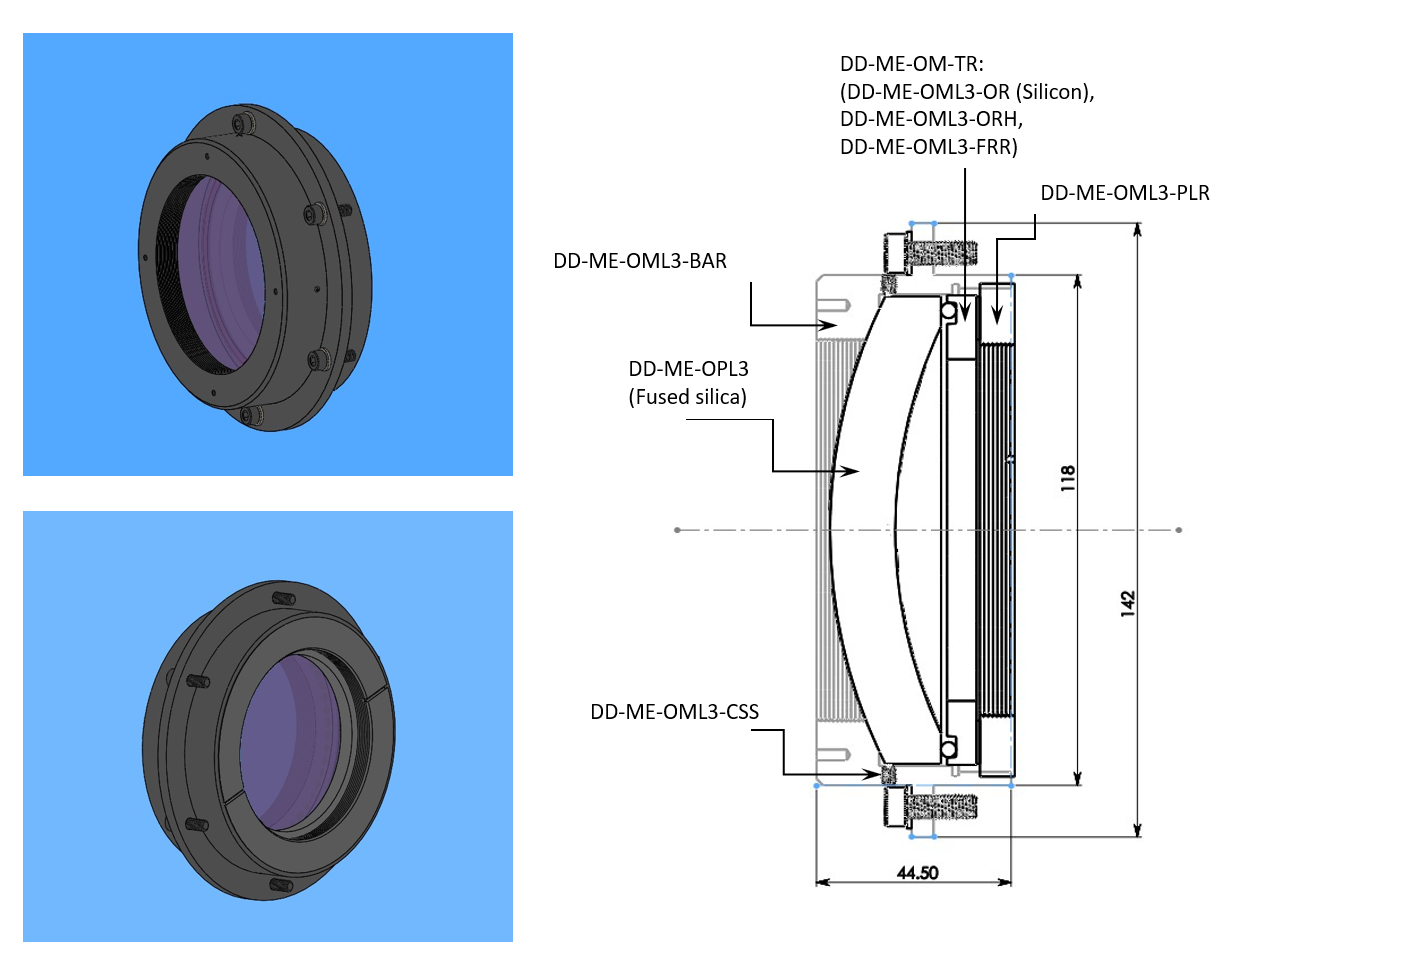
\includegraphics[width=1.1\linewidth]{figures/DD-ME-OML3-ID.png}
\end{center}
\caption{DD-ME-OML3 3d model (front and back views) and cross-section view of the Optomechanical Design.}
\label{figure:OML3-ID}
\end{figure}

\begin{figure}
\begin{center}
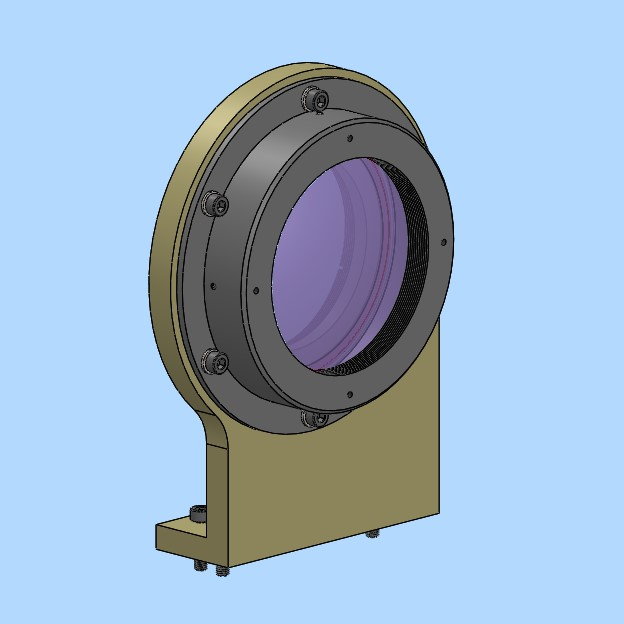
\includegraphics[width=0.7\linewidth]{figures/DD-ME-OML3-PP_w_LBr_2021-12-24.jpg}
\end{center}
\caption{The DD-ME-OML3-BAR barrel mounted on its L-Bracket DD-ME-OML3-LBR.}
\label{figure:OML3-BR}
\end{figure}

The barrel DD-ME-OML3-BAR mounts onto the L-bracket DD-ME-OML3-LBR which in turn is mounted on the plate SS-FP1. The L-bracket has a cut-away to avoid an interference with the optomechanics of L1L2 and D1CP. This is shown in Figure \ref{figure:OML3-BR}.

\section{The DD-ME-OML4 Mount for L4}

L4 is a singlet meniscus lens in Fused Silica with a diameter of 108 mm. It constitutes the red channel field lens. The design of the lens barrel is shown in Figure \ref{figure:OML4-views}. The design of the barrel is almost the same as that for L3, except that the positions of the set-screws are adjusted to match the position of the center of gravity of L4. The barrel DD-ME-OML4-BAR mounts onto the L-bracket DD-ME-OML4-LBR which in turn is mounted on the plate DD-ME-SS-FP1.

The first surface of L4 is convex and contacts with a conical shoulder that is machined in the barrel and provides tangential support. The second surface has a flat bevel in contact with its thermal ring. The cross-section diameter of this O-ring is 3.5 mm (Parker${}^\circledR $2-240). The torque applied with its retaining ring during assembly will give the required pre-load and will compress the O-ring by 21\% at maximum compression.

The barrel has threaded holes for four centering set-screws, giving x and y adjustments for L4. These holes are in the planes of the center of gravity of the lens in order to have a precise control of its position.

\begin{figure}
\begin{center}
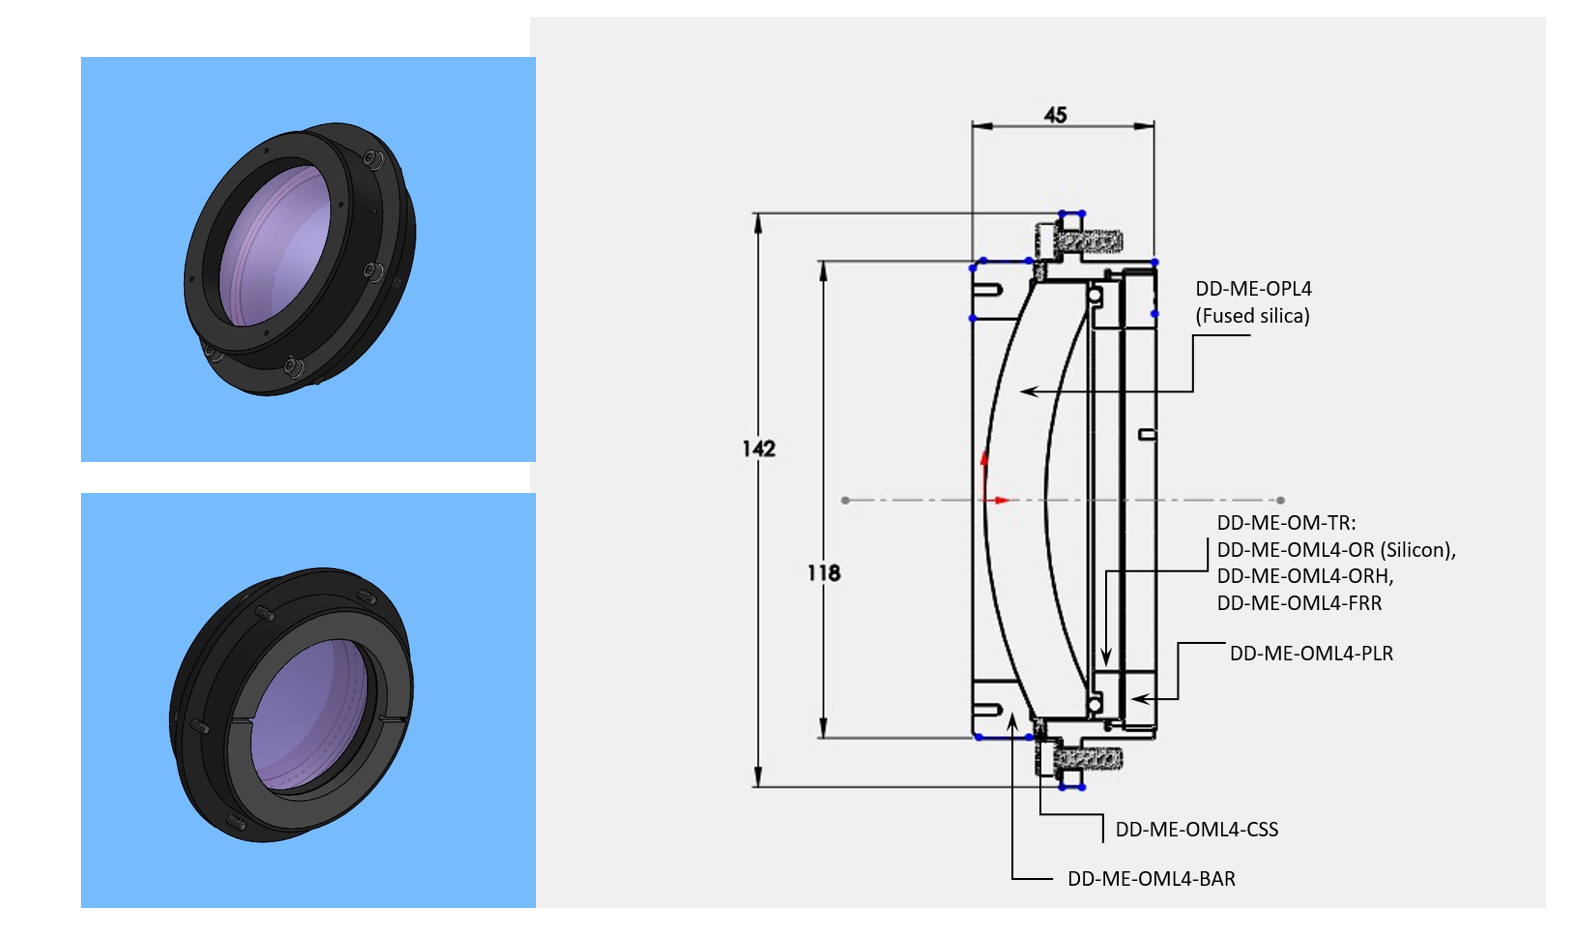
\includegraphics[width=1.1\linewidth]{figures/DD-ME-OML4_ID.png}
\end{center}
\caption{DD-ME-OML4 3d model (front and back views) and cross-section view of the Optomechanical Design.}
\label{figure:OML4-views}
\end{figure}

The L3 and L4 barrels are similar. However, one important difference is that in L4 the mechanical axis of the barrel is inclined by 3 deg with respect to the optical axis of the incoming beam (to compensate the non-axisymmetric aberrations induced by transmission through D2). This requires a slightly wider inner diameter at the entrance of the barrel. The barrel is mounted normally in its L-bracket; the inclination of 3 deg is implemented between the L-bracket and the structural plate FP1. This is shown in Figure \ref{figure:OML4-br}. 

\begin{figure}
\begin{center}
\includegraphics[width=1.1\linewidth]{figures/DD-ME-OML4-BR.png}
\end{center}
\caption{DD-ME-OML4 mounted on its L-bracket and inclination of it with respect to incoming beam.}
\label{figure:OML4-br}
\end{figure}

\section{Mounting DD-ME-OML3 and DD-ME-OML4 on DD-ME-SS-FP1}

The L-brackets of L3 and L4 barrels will be attached to plate DD-ME-SS-FP1. The precise position of the L-brackets on this plate will be achieved during assembly by using a dedicated designed pattern (or template). Appropriate surfaces on this pattern will provide the reference surfaces for precisely positioning the L-brackets (including DD-ME-OMD2), and these will be attached to the plate using screws.

To position the pattern in the right place with respect to DD-ME-SS-FP1, it will have a circular machined tab, concentric to the hole in FP1. While in use, the template will be fixed with screws to FP1. 

\begin{figure}
\begin{center}
\includegraphics[width=1.1\linewidth]{figures/pattern.png}
\end{center}
\caption{Pattern with reference surfaces for the positioning of optomechanical components on fixed plate 1. The pattern will have a machined tab, concentric to the hole in FP1.}
\label{figure:P1_pattern}
\end{figure}


\section{Tolerances}

Table \ref{table:tolerances} shows the translation from the optical tolerances to the mechanical tolerances for OML1L2, OML3, and OML4. Note that the tolerances on OML3 and OML4 are identical. The mechanical tolerances are typically much smaller than formally required by the optical tolerances but are still easily achievable. This large safety factor leaves greater margin for integration tolerances in the support structure and other elements.

\begin{table}
\caption{Tolerances L1 to L4}
\label{table:tolerances}
\begin{center}
\small
\begin{tabular}{lp{2cm}p{2cm}p{6cm}}
\hline
\hline
Component&Optical\par Tolerance&Mechanical\par Tolerance&Comment\\
\hline
L1+L2	
&position\par$\pm0.3$ mm &despace\par$\pm0.05$ mm&
Length. The distance between reference surface A and entrance of barrel must have a symmetrical tolerance of ±0.05 mm.\\
&misalignment\par$\pm0.4$ mm&decenter\par$0.05$ mm&							
Concentricity. The axis of the controlled cylinder must lie within a cylindrical tolerance zone of diameter 0.05 mm and coaxial with reference.\\
&tilt\par$\pm9$ arcmin&tilt\par$0.03$ mm&
Perpendicularity. The axis of the controlled cylinder (barrel) must lie within a cylindrical tolerance zone of diameter 0.03 mm and perpendicular with reference surface A (flange).\\
\hline
L1
&position\par$\pm0.1$ mm&despace\par$\pm0.05$ mm&
Angularity. Controlled plane must lie within two parallel planes 0.05 mm apart. The angle must be theoretically exact.\\	
&misalignment\par$\pm0.3$ mm&decenter\par$0.05$ mm&
Concentricity. The axis of the controlled cylinder must lie within a cylindrical tolerance zone of diameter 0.05 mm and coaxial with reference.\\
&tilt\par$\pm6$ arcmin&tilt\par0.03 mm&Perpendicularity. The axis of the controlled cylinder (barrel) must lie within a cylindrical tolerance zone of diameter 0.03 mm and perpendicular with reference surface A (flange).\\
\hline
L2
&position\par$\pm0.2$ mm&despace\par$\pm 0.05$ mm&
Spacer length. The tolerance on the thickness or length of the spacer determines the despace tolerance of L2. This length must be theoretically exact.\\
&misalignment\par$\pm0.2$ mm&decenter\par0.05 mm&
Concentricity. The axis of the controlled cylinder must lie within a cylindrical tolerance zone of diameter 0.05 mm and coaxial with reference.\\
&tilt\par$\pm6$ arcmin&tilt\par0.05 mm&
Spacer angularity. Controlled plane in spacer must lie within two parallel planes 0.05 mm apart. The angle must be theoretically exact.\\
\hline
L3 and L4											
&position\par$\pm0.2$ mm&despace\par$\pm0.05$ mm&
Length. The distance between reference surface B and entrance of barrel must have a symmetrical tolerance of ±0.05 mm.\\
&&0.1 mm&
Angularity. Controlled plane must lie within two parallel planes 0.1 mm apart. The angle must be theoretically exact.\\
&misalignment\par$\pm1$ mm&decenter\par0.05 mm&
Concentricity. The axis of the controlled cylinder must lie within a cylindrical tolerance zone of diameter 0.05 mm and coaxial with reference.\\	
&tilt\par$\pm30$ arcmin&tilt\par0.04 mm&
Perpendicularity. The axis of the controlled cylinder (barrel) must lie within a cylindrical tolerance zone of diameter 0.04 mm and perpendicular with reference surface B (flange).\\
\hline
\end{tabular}
\end{center}
\end{table}

\section{Manufacture}

The components pending of manufacturing: lens barrel (L4), O-ring holders (L3 and L4), and preload rings (L3 and L4) will be turned conventionally. Both L3 and L4 L-brackets will be manufactured by milling.
We will use the Mitutoyo 7106 Coordinate-Measuring Machine in the IA laboratory to perform metrology of the mechanical pieces. Using an iterative manufacturing process, we can typically achieve 20 $\mu$m precision for the reference surfaces, which is well within the tolerances imposed by the optical design.
The friction-reducing rings will be cut from 1/32-inch thick (approximately 0.8 mm) sheets and glued to the preload rings.

\section{Centering}

Table \ref{table:self-centerability} shows whether each lens is self-centering according to the Karow (\ref{karow}), Hopkins (\ref{hopkins}), and INO (\ref{ino}) criteria. Each lens is self-centering according to at least one criterion and not self-centering according to at least one other criterion.
Therefore, we feel that we cannot reply on the lenses being self-centering.
So, while we will of course take advantage of any tendency of the lenses to self-center, we will explicitly center the lenses in our ALBATROS alignment bench using radially directed nylon-tipped set-screws as a temporarily aid to center the lens in its barrel. 

\begin{table}
\caption{Self-Centerability L1 to L4}
\label{table:self-centerability}
\begin{center}
\small
\begin{tabular}{lccc}
\hline
\hline
Element&Karow&Hopkins&INO\\
\hline
L1&Y&N&Y\\
L2&N&N&Y\\
L3&Y&Y&Y\\
L4&Y&Y&Y\\
\hline
\end{tabular}
\end{center}
\end{table}

Once the lens is aligned, the assembly pre-load (see below) will be applied by means of a threaded pre-load ring until it reaches the required torque. This pre-load maintains the alignment.

After the pre-load is applied, the set-screws are backed off. (The lens barrel contracts more than the lenses at temperatures below the assembly temperature. If the set-screws are not backed off, this can cause a dangerously high stress on the lens.)

This procedure, used while assembling DDRAGUITO, allowed us to center the L1L2 optomechanics to better than 30 microns ($24 \pm 3$ microns), and L3 optomechanics to less than 5 microns. (Ref. \ref{aivDDRAGUITO})


\section{Preload and Thermal Compensation}

The lenses must be supported against axial and radial accelerations of up to 5g. Ultimately, this support is provided by the axial preload modified by the geometry of the lens contact with the barrel and rings. The axial preload is supplied by the threaded preload ring that closes the barrel.

From these requirements, the minimum preload $F_A$ is calculated (\ref{yoder15}) according to
\begin{equation}
\label{Eq:preload}
F_A = \left(\frac{5Mg}{\mu}\right) \cos^2\theta,
\end{equation}
in which $M$ is the mass being supported, $g$ is the acceleration due to gravity, $\mu$ is the coefficient of static friction, and $\theta$ is the inclination of the tangential contact surface.  Values of $M$, $\theta$, and $F_A$ are given in Table \ref{table:minimum-preloads}. We assume $\mu = 0.15$ for aluminium-glass interfaces.

\begin{table}
\caption{Minimum axial preload for lenses L1 to L4}
\label{table:minimum-preloads}
\begin{center}
\small
\begin{tabular}{lllccc}
\hline
\hline
Mount&Interface&Supporting&$$M$$&$\theta$&$F_A$\\
&&&(kg)&(\deg)&(N)\\
\hline
DD-ME-OML1L2&BAR-L1&L1+SPA+L2 &3.123&\phantom{}15.1&\phantom{<}964\\
            &L1-SPA&SPA+L2    &1.624&\phantom{0}0.0&\phantom{}545\\
            &SPA-L2&L2        &1.5&\phantom{}15.3&\phantom{<0}m470\\
\hline
DD-ME-OML3  &BAR-L3&L3        &0.833&\phantom{}24.0&\phantom{<0}86\\
\hline
DD-ME-OML4  &BAR-L4&L4        &0.306&\phantom{}24&\phantom{<0}86.5\\
\hline
\end{tabular}
\end{center}
\end{table}

Some additional comments are warranted for L1+L2. First, the tangential contact between L1 and the barrel must support L1, the spacer SPA, and L2. Second, the contact between L1 and the spacer must support the spacer and L2. Finally, the contact between the spacer and L2 must support L2. Considering the three interfaces, the one that drives the minimum axial preload is the one between the barrel and L1, both because the supported mass is less for the other interfaces and because the $\mu$ will be larger than 0.15 for the interface between the ground bevel of L1 and SPA.

As the temperature changes, the dimensions of the components will change and the axial preload will also change. To reduce this to an acceptable level, we use a passive thermal compensator situated between the last lens and the threaded preload ring. The thermal compensator consists of a soft silicone O-ring (OR), an aluminium holder (ORH), and a friction reducing ring cut from PTFE (Teflon${}^\circledR $) sheet (FRR). The Oring is in contact with a flat ground bevel of the last lens and absorbs most of the axial dimensional variation with temperature. The PTFE friction-reducing ring (FRR) reduces the friction at the interface between the O-ring holder (ORH) and the preload ring (PLR) and will reduce twisting of the O-ring when the preload is applied during assembly.

EPDM and silicone rubber were chosen for the O-rings because of their good heat resistance, good cold flexibility down to -59 C, good weather resistance, and resistance to microbiological growth.

The rate of change of preload with temperature has been considered by calculating the temperature sensitivity factor or $K_3$ for each configuration (\ref{yoder15}). The values of $K_3$, along with the preload at the assembly temperature and extreme survival temperatures, are shown in Table \ref{table:preloads}. Note that the maximum preload varies only very slowly with temperature (because both EPDM and silicone O-rings are an almost perfect thermal compensators), but that formally the maximum preload and hence the maximum stress will occur at the maximum survival temperature of 50 C.

\begin{table}
\caption{Rate of change of preload with temperature for L1 to L4.}
\label{table:preloads}
\begin{center}
\small
\begin{tabular}{lcccc}
\hline
\hline
Mount&$K_3$&$-25$ C&20 C&50 C\\
&($\unit{N\,C^{-1}}$)&N&N&N\\
\hline
DD-ME-OML1L2   &$0.327$&\phantom{}950&\phantom{}964&\phantom{}974\\
DD-ME-OML3     &$0.056$&\phantom{0}84&\phantom{0}86&\phantom{0}88\\
DD-ME-OML4     &$0.056$&\phantom{0}84&\phantom{0}86&\phantom{0}88\\
\hline
\end{tabular}
\end{center}
\end{table}

At assembly, the preload is applied by turning the preload ring to compress the O-ring. After preloading barrels L1+L2 and L3, the resulting compression for the EPDM O-ring of L1+L2 was of 27\% and 21\% for the Silicon O-ring of L3. We expect the compression of the Silicon O-ring of L4 to be the same than that of L3.
These data were compared and are consistent to the characterization we obtained with a Shimadzu compression testing machine at the Faculty of Engineering of the UNAM. The tests consisted of the measurement of sectional compression vs applied force for both EPDM and silicone O-rings.

Considering the thread of the preload ring (M185X2 for OML1L2-PLR and M114X2 for OML3-PLR and OML4-PLR) and the assembly preloads (964 N for OML1L2 and 86 N for both OML3 and OML4), we applied a torque of 35.3 N$\cdot$m for L1L2 barrel, and 3 N$\cdot$m for L3 (the same preload will be applied to L4 barrel).

The preload ring has transverse slots machined into its external face to accommodate the rectangular lugs on a specifically designed bench that allows us to measure and control the preload while turning the preload ring.

\begin{figure}
\begin{center}
\includegraphics[width=0.7\linewidth]{figures/preload_bench.jpg}
\end{center}
\caption{Preload bench with torquemeter.}
\label{figure:ploadB}
\end{figure}

To keep the preload, we will use a thread-locking compound (Loctite${}^\circledR $ 1372603 Blue Thread Locker tape) to secure the preload ring. Using tape rather than liquid has the advantage that there is less risk of damaging a lens.

\section{O-Ring Compression and Set}

The preload will compress the O-rings. It is important that compression is not so much that there is contact between the lens and the O-ring holder at any temperature within the survival range.

The correct performance of DDRAGO’s thermal rings requires a continuous contact annular region between the O-ring and the lens surface. The establishment of this annular region depends on the preload applied and the materials involved. The amount of squeeze (compression) on the O-ring should not produce an excessive deformation of the cushion element. The compression load on each linear inch of an O-ring depends principally on the Shore hardness of the O-ring, its cross-section, and the required preload. In DDRAGO’s lenses, EPDM and silicone O-rings will all have a cross-section diameter of 3.53 mm (0.139 in). The L2 O-ring (with a contact circle of 164 mm diameter) will have a durometer of 70 Shore A and will support a maximum axial preload at 50 C of 974 N, which means a linear preload of 1830 N/m. The L3 O-ring (with a contact circle of 98 mm diameter) will have a durometer of 50 Shore A and will support a maximum axial preload at 50 C of 88 N, meaning a linear preload of 276 N/m.

The maximum squeeze of 27\% on L2 O-ring means a reduction on its diameter of 0.95 mm at maximum survival temperature. Since the distance between the O-ring holder and L2 is 1.53 mm, there will be a clearance of about 0.57 mm, avoiding contact between lens and O-ring holder.

A maximum squeeze of 21.5\% on the L3 and L4 O-rings at maximum survival temperature means a reduction on their diameters of 0.70 mm. Since the distance between the O-ring holders and L3 is 1.43 mm, there will be a clearance of about 0.67 mm, avoiding contact between the respective lenses and O-ring holders. Considering also the temperature dimensional changes of the O-rings, they will experience a change of $\pm 0.025$ mm which is negligible here.

All the glands for DDRAGO’s O-rings have been designed following Parker recommendations, design charts and tables, with the groove outside diameter as primary and the groove inner diameter adjusted to allow a nominal gland fill of 80.7\% for L2 and 80.5\% for L3 and L4.

When under stress, rubber materials experience a progressive relaxation or creep that eventually results in a permanent deformation or “set” (\ref{parker}). The O-ring loses its O-shape causing a discontinuous contact line between the surfaces. Compression Set is determined in air aging and reported by Parker as the percent of deflection by which the elastomer fails to recover after a fixed time under specified squeeze and temperature. Zero percent indicates no relaxation has occurred whereas 100\% indicates total relaxation. See Parker’s Figure 2-9 (\ref{parker}).

Failure by compression set may be caused by several conditions, the more relevant for DDRAGO case are the selection of material and seal cross-section, gland design, and temperature range. Silicone compounds are recommended for static seals whose main requisite is to have a good (low) compression set resistance. Silicone is considered to have ``G/E'' (good to excellent) compression set.
As seen in Parker’s figure 2-15 for both EPDM and Silicone O-rings to be used in DDRAGO, the Compression Set is below 4\% since the maximum survival temperature is 50 C (or 122 F). With respect to temperature conditions, DDRAGO is well within the normal recommended temperature range for EPDM (-50 C to 150 C) and Silicone (-59 C to 204 C).

All these suggest that the selection of O-ring material, the width or cross-section, and preload applied will induce an unimportant deformation on the O-ring, that it will not fail, and that the lenses can be protected by the thermal rings.

\section{Compressive and Tensile Stresses}

The stresses induced within the lenses depend on the preload, the radius of the optical surfaces, the geometric shape of the mechanical interface, and the physical properties of the materials involved.

The lenses in DDRAGO have three types of optomechanical interfaces which help to reduce contact stress:
\begin{enumerate}
\item Tangential interface between conical aluminum surfaces and polished convex lens surfaces (BAR-L1, SPA-L2, BAR-L3 and BAR-L4). Since these are between two precision surfaces, the force is spread over a reasonable area of contact.
\item Flat-bevel interface between flat aluminum surfaces and ground lens bevels (L1-SPA). Here care must be taken that the ground lens bevel is sufficiently flat to avoid restricting the contact to a few high points. This is perfectly feasible with modern grinding machines.
\item Toroidal interface between an O-ring and ground lens bevels (L2-OR, L3-OR and L4-OR). Here the soft O-ring ensures that the force is spread over a reasonable area of contact.
\end{enumerate}

Compressive contact stress at these interfaces is accompanied by tensile stress occurring at the boundary of the region elastically compressed by the applied preload. The relationship between compressive stress $S_c$ and tensile stress $S_T$ is

\begin{equation}
\label{Eq:stress}
S_T = \frac{1}{3}S_C(1-2\nu),
\end{equation}

In which $\nu$ is the Poisson ratio.

The maximum compressive and tensile stresses (at 50 C) are given in Table \ref{table:stress}.

\begin{table}
\caption{Maximum Stresses for lenses L1 to L4 at 50 C}
\label{table:stress}
\begin{center}
\small
\begin{tabular}{lcccc}
\hline
\hline
Lens&Material&Compressive Stress&Tensile Stress\\
&&(MPa)&(Mpa)\\
\hline
L1 &{\CaF}&8.39&1.34\\
L2 &N-BaK4&8.61&1.49\\
L3 &Fused Silica&5.38&1.22\\
L4 &Fused Silica&5.26&1.19\\
\hline
\end{tabular}
\end{center}
\end{table}

\section{Failure Probability}\label{secFailProb}

The probability of mechanical failure of a lens depends largely on the tensile stress. The maximum tensile stresses are shown in Table \ref{table:stress} and occur at 50 C. The largest value is 1.49 MPa.

For simplicitly, we will assume that all of the lenses L1 to L11 suffer a maximum tensile stress of 1.50 MPa, even though some will have lower stresses. 
In the case of the cemented doublet Ca$F_2$-SFTM16, it will be considered for this calculation Ca$F_2$ glass, which is more sensitive than SFTM16.

Using Weibull statistics, we can estimate the probability of failure when this maximum stress is applied as $3.1 \times 10^{-8}$ for each Fused Silica lens (L3, L4, L7), $9.8\times 10^{-10}$ for each Ca$F_2$ lens (L1, L5, L6, L8, L11), and less than $10^{-12}$ for each N-BaK4 (L2) and S-FTM16 (L9, L10) lenses.

Since the values of $K_3$ for the optomechanical designs are so small, the stress on the lenses does not change dramatically from day (warmer – higher stress) to the night (colder – lower stress). Nevertheless, we will assume that each day the lenses are taken to the maximum stress and this is then released.

From this, we can calculate the combined probability of at least one failure in all eleven warm lenses when the maximum stress is applied as $8.4 \times 10^{-8}$.

If we assume that the instrument is heated up to the maximum survival temperature (50 C) every day, then the probability of at least one warm lens failing during the 10-year life of the instrument is $3.7\times 10^{-4}$. So, even in this highly unlikely scenario, the probability of a failure is negligible.

\chapter{DDRAGO Dichroic and Corrector Plate Optomechanics Design}

\section{Tower}

The tower is an assembly of structural and optomechanical elements designed to support the D1 dichroic and CP corrector plate. It connects to the P1 plate. Figure~\ref{figure:tower-general} shows a general view of the tower and illustrates a key driver in the design: avoiding mechanical interferences with D2, L3, L4, and the blue and red filter wheels and avoiding vignetting of the multiple optical beams in this space.

\begin{figure}
\begin{center}
\includegraphics[width=0.8\linewidth]{figures/tower-general.png}
\end{center}
\caption{General view of the tower showing D1 and CP (in the tower) and D2, L3, and L4 (attached to P1).}
\label{figure:tower-general}
\end{figure}

The tower has four structural parts: the interface ring, the two lateral plates, and the rear plate. See Figures~\ref{figure:tower-close}, \ref{figure:tower-section}, \ref{figure:tower-front}, and \ref{figure:tower-rear}. They are fabricated from Alumold, which is equivalent to a 7000-series aluminium and is well suited to high-precision machining. The structural parts will be joined by screws.

\begin{figure}
\begin{center}
\includegraphics[width=0.8\linewidth]{figures/tower-close.png}
\end{center}
\caption{The strutural parts of the tower.}
\label{figure:tower-close}
\end{figure}

The lateral plates serve to give rigidity to the assembly. Both have a specific shape, designed to be light but strong. One of them has a cut-out designed to avoid mechanical interference with the L3 mount and barrel and with the motor of the blue filter wheel (see Figure~\ref{figure:tower-general}).

Attaching the tower to the plate P1 was a challenge. We wish to reuse the L1L2 barrel from DDRAGUITO without modification (since modifications would require removing the lenses, including the enormously expensive CaF2 L1), and so the best solution we found was to design an interface ring to fit over the back of the barrel and place a 4.5 mm spacer ring between the barrel and P1. This can be seen in \ref{figure:tower-section}. Screws from the rear then pass through the interface plate, the flange on the L1L2 barrel, and the spacer ring, and finally into the P1 plate

The tower gives the precise positions and inclinations for D1 and CP by design and CNC machining of the lateral plates. The annular interface plate of the tower has a circular distribution of holes which provides concentricity with the circular aperture on the structural plate 1 with an integration tolerance of ± 0.06 mm (plane X-Y) given by the specified fits, which is well below the optical tolerances (±0.150 mm for D1 and ±1 mm for CP). This concentricity will be verified by metrology.

During the assembly of D2, L3 and L4 mounts on the structural plate 1, we will use a precision template with reference surfaces to put them in the specified position (for more details, please refer to Section 5.5). The machining precision of the reference surfaces of the template is 50 microns, which is well below the optical tolerances.

\begin{figure}
\begin{center}
\includegraphics[width=0.7\linewidth]{figures/tower-section.png}
\end{center}
\caption{Sectional view of the tower and L1L2 barrel.}
\label{figure:tower-section}
\end{figure}
 

\begin{figure}
\begin{center}
\includegraphics[width=0.7\linewidth]{figures/tower-front.jpg}
\end{center}
\caption{Front view of the tower}
\label{figure:tower-front}
\end{figure}

\begin{figure}
\begin{center}
\includegraphics[width=0.7\linewidth]{figures/tower-rear.jpg}
\end{center}
\caption{Rear view of the tower.}
\label{figure:tower-rear}
\end{figure}

\section{D1 and CP Holders}

D1 and CP have  wedges. Therefore, some care needs to be taken to accommodate them in their holders. We adapted the design from the holders for the RATIR 

Figure \ref{figure:tower-d1-lower} shows how D1 is inserted into its holder. The orthogonal (non-wedged) lower surface of D1 is placed into the holder. The holder is manufactured from Alumold. The dichroic is protected from surface roughness by a 250 {\micron} Mylar liner. It is held laterally by two nylon-tipped set screws which push it against two contact bumps on the long side and one on the short side. 

The axial support is shown in Figure~\ref{figure:tower-d1-upper}.
The dichroic protrudes slightly above the upper surface of the frame. The height of the protrusion is not constant because dichroic is wedged but the frame is not. Axial support is provided by black nylon strips, 0.8 mm thick, which are pushed against the upper surface of the dichroic by pressure bars, manufactured from aluminum plate, and screws.


\begin{figure}
\begin{center}
\includegraphics[width=0.7\linewidth]{figures/tower-d1-lower.png}
\end{center}
\caption{The D1 holder showing the lateral contact bumps and set screws and the Mylar liner.}
\label{figure:tower-d1-lower}
\end{figure}


\begin{figure}
\begin{center}
\includegraphics[width=0.7\linewidth]{figures/tower-d1-upper.png}
\end{center}
\caption{The D1 holder showing the nylon strips, pressure bars, and screws that give axial support.}
\label{figure:tower-d1-upper}
\end{figure}


The same design concept is used for the CP holder.

The D1 and CP holders are screwed into the tower between the two lateral plates.

The holders of D1 and CP will act as additional elements to the structure-tower as well. This means that the tightening torque of the screws must be well controlled during their assembly.

\section{D2 Support}

The wedged D2 dichroic is supported in a holder following the same concept as the D1 holder. However, as Figure~\ref{figure:d2-general} shows, the holder is extended to also serve as an L-bracket. This will be attached directly to P1.

\begin{figure}
\begin{center}
\includegraphics[width=0.7\linewidth]{figures/d2-general.png}
\end{center}
\caption{The D2 combined holder and L-bracket}
\label{figure:d2-general}
\end{figure}

\section{Manufacture}

Most of the aluminium pieces will be manufactured using the CNC machine in our workshop. The exceptions are the interface ring and spacer ring, which will be manufactured conventionally in our workshop using a lathe. Because the main material used for manufacturing the instrument is aluminium, no release treatment is required.

The nylon strips and Mylar liners will be cut by laser. To give clean edges, we will sandwich the nylon and Mylar sheets between thin wooden sheets.

The pressure bars will be cut from aluminum plate on a conventional milling machine.

\chapter{DDRAGO Detector Supports}


\section{Requirements}

We need to be able to statically adjust the CCDs in focus (so that they can both be focused by the telescope secondary), tilt (to maintain focus across the field), and lateral position (to align the field centers). 

For this, the removable plates containing the CCDs have adaptors designed to provide adjustment in focus and tilt while maintaining sufficient stiffness against flexure. The plates are mounted to the support structure in a way that allows a repeatable adjustment laterally. The filter wheel is attached to the inside of the removable plate. These removable plates have two handles (McMaster part 1979A300) to ease their manipulation. The mass of the each plate, with the detector and filter wheel, is approximately 20.6 kg.

\section{Focus and Tilt Adjustment}

The mount design, which is the same used for DDRAGUITO, uses three M12 bolts that act between an adapter ring (attached to the detector head) and one of the Support Structure removable plates. The attachment to the removable plates uses spherical washers to allow the bolts to tilt as well as extend.

Normally, the play in the bolt thread would limit the precision with which we could position the detector. To counteract this, after adjustment, the threads in the adapter ring are tightened on the M12 bolt using two lateral tightening bolts (see Figure \ref{figure:SSCCDmounts}). We have verified that this reduces the play to about 5 micrometers, which is now negligible. The play between the M12 bolt and the removable plate is also eliminated by the use of locking nuts on both sides of the spherical washers.

The gap between the adapter ring and the removable plate is sealed against light in two ways. First, the adapter ring has an extension into the removable plate which acts as a baffle. Second, we will place a compressible black EVA foam liner cut from 3/8-inch thick sheet (McMaster part 86095K43) between the ring and the plate. The design uses Alumold 500 (although an equivalent 7000-series alloy could be substituted if need be), suitable for precision machining. We will manufacture the aluminum parts in our CNC machine.

We made metrology of the movements of the Tip/Tilt mechanism during the verification of DDRAGUITO in our laboratories in 2019. The accuracy results were 5 micrometers along the optical axis, and an inclination of 15 arcseconds of the detector plane. The plates DD-Cg-ME-SS-P5T/P6T, shown in Figure \ref{figure:SSCCDmounts2}, support the blue detector mount (DD-Cg-ME-CAR/CAB-TipTilt) and the blue filter wheel (DD-Cg-ME-SS-BFW/RFW). 


\begin{figure}
\centering
\includegraphics[width=1\linewidth]{figures/SSCCDmounts.png}
\caption{Blue and Red CCD mounts, showing the compressible black EVA foam (1) and the baffle (2).}
\label{figure:SSCCDmounts}
\end{figure}

\begin{figure}
\centering
\includegraphics[width=1\linewidth]{figures/SSCCDmounts2.png}
\caption{Blue (3) and red (2) detectors with Tip/Tilt mechanism positioned at the plates SS-P10 and SS-P7 respectively.}
\label{figure:SSCCDmounts2}
\end{figure}

\section{Lateral Adjustment}

The lateral adjustment is used for centering the detector with the light beam coming from the telescope. For this purpose, the pushing hardware is used. Each detector mount has three of these mechanisms fixed to the main structure. The positions are shown in Figure \ref{figure:PushMounts}.

The procedure for centering is placing the mount in its corresponding plate. Then, with all screws tight, it is necessary to calibrate the Focus and Tilt adjustments (see previous Section). After, the screws of fixation require to be loosen enough to allow lateral movements but always maintaining the contact between the mount and its plate. The movement can be checked pushing by hand. The distance of movement is 1 mm to each side. Before moving the pushing hardware, the mount has to be moved (by hand) until the mount reaches the inside walls, closer to the pushing hardware, of its structural plate. Once in this position, the M4 set screw can be used for centering the detector and the beam light. The resolution is related with the M4 set screw thread pitch of 0.7 mm.

\begin{figure}
\centering
\includegraphics[width=1\linewidth]{figures/PushMounts.png}
\caption{Lateral adjustment.}
\label{figure:PushMounts}
\end{figure}

\chapter{DDRAGO Detector Dummies}

We need dummies for the DDRAGO detectors to maintain the instrument balance even if one or both real detectors need to be removed for maintenance.

The dummies have been designed considering that each detector has a mass of 12.6 kg and its center of mass is at 88 mm from the coupling flange.

Figure \ref{figure:ccd-dummy} shows a 3D model of the dummy and an exploded view.

\begin{figure}
    \centering
    \includegraphics[width=0.7\linewidth]{figures/CCD-dummy.png}
    \caption{The CCD dummies}
    \label{figure:ccd-dummy}
\end{figure}

The parts of the dummy are: 
\begin{itemize}
    \item a coupling flange (nylon plate) 
    \item three fully threaded studs (commercial parts M12x1.75 stainless steel T-304)
    \item stainless steel nuts and washers
    \item a counterweight (cold rolled steel 5 inches in diameter)
    \item a back plate (nylon plate)
\end{itemize}

The dummy flange has the same dimensions and holes distribution than the detector flange, so it can be assembled to the instrument in the same place as the detector.

The three studs are 30 cm long and will be distributed at 120 degrees. These will be fastened to the front flange and back plate using nuts and washers. In the middle, the position of the counterweight will also be fastened by nuts and washers.

The free room between the front and back plates allows to modify the position of the counterweight, having the possibility to adjust the position of the center of mass in a range between 65 mm and 90 mm from the coupling flange. This is shown in Figure \ref{figure:ccd-dummy-adjustment}.

\begin{figure}
    \centering
    \includegraphics[width=0.7\linewidth]{figures/CCD-dummy-range.png}
    \caption{The range of adjustment of the center of mass of the CCD dummy}
    \label{figure:ccd-dummy-adjustment}
\end{figure}

\chapter{WOB Design}

The Warm Optical Bench (WOB) has been designed as an independent module which means that lenses L5 to L11 as well as the three folder mirrors are going to be attached to a single structural plate. This is convenient since the WOB will be installed in the instrument after DDRAGO is installed at the telescope and it will allow aligning these optics in an optical bench at laboratory.

Here we describe the general design of the plate, the optomechanical design proposed for the seven WOB lenses and three folder-mirror mounts that carry the beam coming from DDRAGO and into the infrared cryostat.

Some special features should be included in the optomechanical design: a pin-hole, a field mask, a shutter and a focusing mechanism. Of the three mounts for the mirrors, two of them should have kinematic mounts to be used when aligning the optical system.

\begin{figure}
\begin{center}
\includegraphics[width=0.7\linewidth]{figures/WOB_layout.png}
\end{center}
\caption{WOB optomechanical layout.}
\label{figure:WOB-LO}
\end{figure}

We begin by summarizing the design considerations, we then present the design of the WOB plate, then the optomechanical design, first in a general sense and then individually for the single lenses L5, L6, L7, the cemented doublet L8L9 and the singlets L10 and L11. We then discuss the corresponding tolerances, the centering method, the thermal compensation, manufacturing processes and the required preloads.

The mountings for the folder mirrors are presented in a subsequent chapter.

Likelihood of failure due to stresses was already discussed in Section \ref{secFailProb}.

\section{Considerations and General Design}

The optomechanical design presented here was developed according to the following specifications established by the optical design and integration convenience:
\begin{enumerate}
\item All of the WOB CAGIRE optics will be mounted on the same structural plate (DD-ME-WOB-PL), and attached inside the instrument structure. This will allow us to integrate the optomechanical components on the plate and finally integrate the plate into the instrument support structure. 
\item Folder mirrors FM1 and FM2 will be used for aligning, so these will have kinematic mountings. 
\item The lens materials are Ca$F_2$, Fused Silica and SFTM16.
\item The barrels should provide an attachment flange to allow them to be fixed to L-brackets and these to the WOB plate.
\item Whenever necessary, the barrels will have vent holes machined in the body to allow for the adequate assembly of lenses.
\item The inner diameter at the entrance of each barrel will have an appropriate dimension so to act as a baffle. Furthermore, the inner surfaces of the barrel and aluminium rings will be grooved with a triangular pattern and 800 microns height (see Figure \ref{figure:rosalia-grooves}).
\item The first and second folder-mirrors FM1 and FM2 will be used for aligning the WOB optical layout, so they must have the possibility of being aligned.
\item A pinhole should be placed at the focal plane of the telescope, located before lens L5. The pinhole should be removable since it will only be used during alignment.
\item The barrel of lens L5 should permanently hold a field mask 
\item A shutter should be placed near lens L5 since that is the region where the beam is narrower.
\item The focusing of the system will be carried out by shifting lens L7 
\item The cemented doublet L8L9 and the single lenses L10 and L11 will be located in a same barrel 
\item The tolerances in axial positioning, decentering, and tilts are given by the optical design
\item The alignment and verification of lenses inside their respective barrels will be carried out with the IA-UNAM aligning system ALBATROS.
\item The calculated preload on lenses in their barrels will be applied in a controlled and measured manner 
\item Mechanical parts and lenses will be manufactured, measured and integrated at a temperature of about 20 C
\item The operational temperature range is -15 C to 20 C.
\item The survival temperatures is from -25 C to 50 C.
\item The optomechanical design must protect the lenses and keep their alignment against accelerations of $5g$. (The requirement is that the instruments must survive accelerations of $10g$ during transport, but we assume that the packing will reduce an external $10g$ acceleration sufficiently that a maximum of $5g$ will be imparted to the instrument.)
\item All barrels should have front and rear covers for protection during handling and transport
\item The WOB with the optomechanics included, shall allow its manipulation so it can be mounted and dismounted from the instrument.
\end{enumerate}

Tables \ref{table:WOB-product-tree1}, \ref{table:WOB-product-tree2} and \ref{table:WOB-product-tree3} show an extract of the WOB Product Tree table relevant for the optics supports

\begin{table}
\caption{Extract of the Product Tree Table Relevant for the Optics Mounts from DD-ME-WOB-PL to DD-ME-OML6.}
\label{table:WOB-product-tree1}
\begin{center}
\footnotesize
\begin{tabular}{ll}
\hline
\hline
Code                &Description\\
\hline
DD-ME-WOB-PL	&	WOB Plate\\
DD-ME-WOB-GL	&	WOB Guide-Long\\
DD-ME-WOB-GS	&	WOB Guide-Short\\
DD-ME-WOB-MS1	&	WOB Mechanical Stop 1\\
DD-ME-WOB-MS1-FS	&	WOB Mechanical Stop Fixing Screws\\
DD-ME-WOB-MS2	&	WOB Mechanical Stop 2\\
DD-ME-WOB-MS2-FS	&	WOB Mechanical Stop Fixing Screws\\
DD-ME-WOB-MS3	& WOB Mechanical Stop 3\\
DD-ME-WOB-MS3-FS	& WOB Mechanical Stop 3 Fixing Screws \\
DD-ME-WOB-MS4	&	WOB Mechanical Stop 4	\\
DD-ME-WOB-MS4-FS	&	WOB Mechanical Stop 4 Fixing Screws	\\
DD-ME-WOB-EB1	&	WOB Eyebolt 1	\\
DD-ME-WOB-EB1-FS	&	WOB Eyebolt 1 Fixing Screws	\\
DD-ME-WOB-EB2	&	WOB Eyebolt 2	\\
DD-ME-WOB-EB2-FS	&	WOB Eyebolt 2 Fixing Screws	\\
\hline
DD-ME-OMFM1	&	Optomechanics for FM1	\\
DD-OP-FM1	&	Folder Mirror 1	\\
DD-ME-OMFM1-BR 	&	Bracket	\\
DD-ME-OMFM1-KMH 	&	Kinematic Mounting Holder	\\
DD-ME-OMFM1-KM 	&	Kinematic Mounting	\\
DD-ME-OMFM1-IP 	&	Interface Plate to FM1	\\
DD-ME-OMFM1-OR 	&	O-Ring	\\
DD-ME-OMFM1-SC 	&	Security Cover	\\
\hline
DD-ME-OML5	&	Optomechanics for L5	\\
DD-ME-OML5-LBR	&	L-Bracket	\\
DD-ME-OML5-BAR	&	Barrel	\\
DD-OP-L5	&	Lens 5	\\
DD-ME-OML5-OR	&	O-Ring (Silicone)	\\
DD-ME-OML5-ORH	&	O-Ring Holder	\\
DD-ME-OML5-FRR	&	Friction-Reducing Ring (PTFE)	\\
DD-ME-OML5-PLR	&	Pre-Load Ring	\\
DD-ME-OML5-CSS	&	Centering Set-Screw	\\
DD-ME-OML5-FMSK	&	Field Mask	\\
DD-ME-OML5-PH	&	Pinhole	\\
DD-ME-OML5-PHCN	&	Pinhole Container	\\
DD-ME-OML5-PHCV	&	Pinhole Cover	\\
DD-ME-OML5-SH	&	Shutter	\\
DD-ME-OML5-SHH	&	Shutter Holder	\\
\hline
DD-ME-OML6	&	Optomechanics for L6	\\
DD-ME-OML6-LBR	&	L-Bracket	\\
DD-ME-OML6-BAR	&	Barrel	\\
DD-OP-L6	&	Lens 6	\\
DD-ME-OML6-OR	&	O-Ring (Silicone)	\\
DD-ME-OML6-ORH	&	O-Ring Holder	\\
DD-ME-OML6-FRR	&	Friction-Reducing Ring (PTFE)	\\
DD-ME-OML6-PLR	&	Pre-Load Ring	\\
DD-ME-OML6-CSS	&	Centering Set-Screw	\\
\hline
\end{tabular}
\end{center}
\end{table}

\begin{table}
\caption{Extract of the Product Tree Table Relevant for the Optics Mounts from DD-ME-OML7 to DD-ME-OML8L9.}
\label{table:WOB-product-tree2}
\begin{center}
\small
\begin{tabular}{ll}
\hline
\hline
Code                &Description\\
\hline
DD-ME-OML7	&	Optomechanics for L7	\\
DD-ME-OML7-LBR	&	L-Bracket	\\
DD-ME-OML7-BAR	&	Barrel	\\
DD-OP-L7	&	Lens 7	\\
DD-ME-OML7-OR	&	O-Ring (Silicone)	\\
DD-ME-OML7-ORH	&	O-Ring Holder	\\
DD-ME-OML7-FRR	&	Friction-Reducing Ring (PTFE)	\\
DD-ME-OML7-PLR	&	Pre-Load Ring	\\
DD-ME-OML7-CSS	&	Centering Set-Screw	\\
DD-ME-OML7-FM	&	Focuser Mechanism	\\
\hline
DD-ME-OMFM2	&	Optomechanics for FM2	\\
DD-OP-FM2	&	Folder Mirror 2	\\
DD-ME-OMFM2-BR 	&	Bracket	\\
DD-ME-OMFM2-BMS	&	Bracket Middle Support	\\
DD-ME-OMFM2-BBS 	&	Bracket Bottom Support	\\
DD-ME-OMFM2-KMH 	&	Kinematic Mounting Holder	\\
DD-ME-OMFM2-KM 	&	Kinematic Mounting	\\
DD-ME-OMFM2-IP 	&	Interface Plate to FM2	\\
DD-ME-OMFM2-OR 	&	O-Ring	\\
DD-ME-OMFM2-SC	&	Security Cover	\\
\hline
DD-ME-OMFM3	&	Optomechanics for FM3	\\
DD-OP-FM3	&	Folder Mirror 3	\\
DD-ME-OMFM3-BR 	&	Bracket	\\
DD-ME-OMFM3-OR 	&	O-Ring	\\
DD-ME-OMFM3-SC 	&	Security Cover	\\
\hline
DD-ME-OML8L9	&	Optomechanics for L8L9	\\
DD-ME-OML8L9L10L11-LBR	&	L-Bracket	\\
DD-ME-OML8L9-BAR	&	Barrel	\\
DD-OP-L8	&	Lens 8	\\
DD-OP-L9	&	Lens 9	\\
DD-ME-OML8L9-OR	&	O-Ring (Silicone)	\\
DD-ME-OML8L9-ORH	&	O-Ring Holder	\\
DD-ME-OML8L9-FRR	&	Friction-Reducing Ring (PTFE)	\\
DD-ME-OML8L9-PLR	&	Pre-Load Ring	\\
DD-ME-OML8L9-CSS	&	Centering Set-Screw	\\
\hline
\end{tabular}
\end{center}
\end{table}

\begin{table}
\caption{Extract of the Product Tree Table Relevant for the Optics Mounts of DD-ME-OML10L11.}
\label{table:WOB-product-tree3}
\begin{center}
\small
\begin{tabular}{ll}
\hline
\hline
Code                &Description\\
\hline
DD-ME-OML10L11 & Optomechanics for L10L11\\
DD-ME-OML10L11-BAR	&	Barrel	\\
DD-ME-OML10L11-PF	&	Provisional Flange	\\
DD-OP-L10	&	Lens 10	\\
DD-ME-OML10-OR	&	O-Ring (Silicone)	\\
DD-ME-OML10-ORH	&	O-Ring Holder	\\
DD-ME-OML10-FRR	&	Friction-Reducing Ring (PTFE)	\\
DD-ME-OML10-PLR	&	Pre-Load Ring	\\
DD-ME-OML10-CSS	&	Centering Set-Screw	\\
DD-OP-L11	&	Lens 11	\\
DD-ME-OML11-OR	&	O-Ring (Silicone)	\\
DD-ME-OML11-ORH	&	O-Ring Holder	\\
DD-ME-OML11-FRR	&	Friction-Reducing Ring (PTFE)	\\
DD-ME-OML11-PLR	&	Pre-Load Ring	\\
DD-ME-OML11-CSS	&	Centering Set-Screw	\\
\hline
\end{tabular}
\end{center}
\end{table}
Table \ref{table:WOB-Phys-Prop} gives the physical properties of the materials used: the thermal expansion coefficient $\alpha$, the Poisson ratio $\nu$, the modulus of elasticity $E$, and density $\rho$.


\begin{table}
\caption{Physical Properties of Materials}
\label{table:WOB-Phys-Prop}
\begin{center}
\small
\begin{tabular}{lccccl}
\hline
\hline
Material	&	$\alpha$	&	$\nu$ &	$E$
&	$\rho$ &	Reference\\
&
\unit{C^{-1}}&
&
Pa&
\unit{g\,cm^{-3}}&
\\
\hline
Ca$F_2$	&	$1.885\times10^{-5}$	&	0.26	&	$7.580\times 10^{10}$	&	3.18	&	oharacorp.com	\\
Fused Silica	&	$5.000 \times 10^{-7}$	&	0.16	&	$7.270 \times 10^{10}$	&	2.20	&	corning.com	\\
SFTM16	&	$9.00 \times 10^{-6}$	&	0.238	&	$6.53 \times 10^{10}$	&	2.64	&	oharacorp.com	\\
Alumold${}^\circledR $ 500	&	$2.37 \times 10^{-5}$	&	0.33	&	$7.2 \times 10^{10}$	&	2.82	&	carrs-tool.co.uk	\\
Silicone	&	$1.80\times 10^{-4}$	&	0.5	&	$8.5\times 10^{5}$	&	1.1	&	parker.com	\\
PTFE	&	$19 \times 10^{-5}$	&	0.46	&	$5.4\times 10^{8}$	&	2.15	&	dmh.at	\\
UHMW-PE${}^\circledR$	&	$1.2\times 10^{-4}$	&	0.4	&	$5\times 10^{8}$	&	0.93	&	azom.com\\
\hline
\end{tabular}
\end{center}
\end{table}

\section{The WOB Plate, Guides and Mechanical Stops}

The geometry of the WOB plate has been adapted to follow the beam path from the first folder mirror (FM1) until lens L11.

Folder mirror FM1 receives the beam coming from the corrector plate (CP) and folds it towards L5, following through L6 and L7, then it finds folder-mirrors FM2 and FM3 and, afterwards, the group formed by lenses L8L9, L10 and L11.
 
The WOB plate will support an approximate weight of 26.5 kg (coming from the optomechanical elements) with a center of mass located in a plane parallel to its front face and gravity acting on that same plane.

The WOB plate will provide precisely machined reference surfaces for placing each of the L-brackets and mirror supports in the specified position of the optical layout. It also has grooves for guiding the cables of the shutter and the focuser and an aperture for the focuser connector and cable. Cables will be guided and fixed to the back surface of the WOB using cable clamps.

\begin{figure}
\begin{center}
\includegraphics[width=0.7\linewidth]{figures/WOB_plate.png}
\end{center}
\caption{WOB plate with mechanical stops (MS), mechanical guides (MG), and eyebolts.}
\label{figure:WOB_plate}
\end{figure}

It will be machined from an Alumold${}^\circledR$ plate and its general dimensions are $L=687$ mm, $W=589$ mm with a thickness of 16 mm. It will be rabbeted to lower its weight to approximately 9 kg and a pair of eyebolts can be fastened to the plate to facilitate its handling with a winch.

When putting it into the instrument in the correct position, it will slide on two lateral guides and its position defined and fixed with four mechanical stops. The guides and mechanical stops will be fixed in the instrument structure.

The lateral guides will be made from UHMW-PE, a polyethylene with auto-lubricated surface of very low coefficient of friction and low density. This material is an engineering plastic which makes it suitable for machining. Furthermore, the mechanical stops will be milled machined from Alumold${}^\circledR$ bar.

The function of the mechanical stops is to provide the mechanical alignment of the WOB with DDRAGO.

There are four mechanical stops screwed to the structure that will determine the placement of the WOB (see Figure \ref{figure:MS-WOB}).

\begin{figure}
\begin{center}
\includegraphics[width=0.7\linewidth]{figures/Mechanical-stops-struct.png}
\end{center}
\caption{Four mechanical stops and WOB plate in DDRAGO structure.}
\label{figure:MS-WOB}
\end{figure}


Each mechanical stop has precision reference surfaces to be in contact with the WOB. These surfaces will be CNC machined and CMM measured matching the structure metrology.

The WOB plate has threaded holes to be screwed to the mechanical stops, so the assembly and adjustment of these to the structure is through oversized holes in the mechanical stop and oversized washers in the structure (see Figure \ref{figure:MS-DET}).

\begin{figure}
\begin{center}
\includegraphics[width=0.7\linewidth]{figures/Mechanical-stops-detail.png}
\end{center}
\caption{Fixing and adjustment of mechanical stops.}
\label{figure:MS-DET}
\end{figure}


\section{The DD-ME-OML5 Optomechanical Design}

L5 is a singlet meniscus lens in Ca$F_2$ with a diameter of 90 mm and a weight of 0.225 kg. It is placed after the first folder mirror (FM1) and the telescope focal plane. 

The second surface of L5 is convex and contacts with a conical shoulder that is machined in the barrel and provides tangential support. The first surface is concave and has a flat bevel in contact with its Silicone thermal ring. The cross-section diameter of this O-ring is 3.5 mm (McMaster${}^{\circledR}$ part 1173N235 dash number 235. Hardness durometer 50A). The torque applied with its retaining ring during assembly will give the required pre-load and will compress the O-ring by 15\% at maximum compression.

The barrel has threaded holes for four centering set-screws, giving $x$ and $y$ adjustments for L5. These holes coincide with the plane of the center of gravity of the lens in order to have a precise control of its position when centering with ALBATROS.

\begin{figure}
\begin{center}
\includegraphics[width=1.1\linewidth]{figures/DD-OML5.png}
\end{center}
\caption{DD-ME-OML5 3d model (front and back views) and cross-section view of the Optomechanical Design.}
\label{figure:WOB_OML5}
\end{figure}

The barrel DD-ME-OML5-BAR mounts onto the L-bracket DD-ME-OML5-LBR which in turn is mounted on the plate DD-ME-WOB-PL. The flange of the barrel, the L-bracket and the WOB have reference surfaces for accurately positioning the lens in the WOB. 

\begin{figure}
\begin{center}
\includegraphics[width=0.7\linewidth]{figures/DD-OML5-LBr.jpg}
\end{center}
\caption{DD-ME-OML5 mounted on its L-bracket.}
\label{figure:WOB_OML5_LBr}
\end{figure}

As all the barrels on the WOB, this will have front and rear covers for transport, made from nylon. The front cover will be fixed with screws to the barrel and the rear cover will be fixed to the shutter cover.

The place of this lens in the optical layout implies that its barrel will also enclose a removable pinhole, a field mask and a shutter. 

\subsection{Removable pinhole on DD-ME-OML5-BAR}

When aligning the optics of the WOB, a pinhole is needed in the place where the focal plane of the telescope is situated. This pinhole will be used only for this task and then it will be removed.

A commercial precision pinhole has been chosen from Edmund Optics${}^\circledR $ (56-291) with an aperture diameter of 1 mm. It comes in a stainless-steel mounting (outer diameter: 25 mm) that will be attached to a holder designed to be assembled to L5-BAR.

The holder consists of two pieces: a container and a cover, and between them the pinhole is placed.

The pinhole holder is threaded on its outer diameter matching an inner thread of the barrel. This allows placing the pinhole in the correct position.

\begin{figure}
\begin{center}
\includegraphics[width=1.1\linewidth]{figures/DD-ME-OML5-PH_VEx.png}
\end{center}
\caption{DD-ME-OML5 with removable pinhole.}
\label{figure:WOB-L5-PH}
\end{figure}

\subsection{WOB Field Mask on DD-ME-OML5-BAR}

At the entrance of the L5-BAR, a field mask will be located. It has a squared aperture (56x56 mm) in a circular aluminium sheet. 

The field mask will be screwed to the barrel but, being squared, it must allow to be rotated, so it will have circular slots to adjust its position. To facilitate this task, the field mask will have a pair of pins that will help to rotate the mask with the fingers without risking the lens.

\begin{figure}
\begin{center}
\includegraphics[width=0.7\linewidth]{figures/DD-ME-OML5-FMSK.png}
\end{center}
\caption{DD-ME-OML5 with field mask.}
\label{figure:WOB-L5-FM}
\end{figure}

\subsection{WOB Shutter on DD-ME-OML5-LBR}

Just after L5-BAR, there is a commercial optical shutter (90mm. Vincent/Uniblitz${}^\circledR$ CS90). It comes unmounted, so a Nylamid${}^\circledR$ cover was designed to provide it with a mounting surface.

The shutter in its cover will be screwed to the L5 L-bracket, on the opposing face to the barrel.

This shutter uses a Lemo connector (fgg. 1b 314) that will be attached to the shutter cover. Its cable will be guided through the back face of the WOB and into the Roxtec${}^\circledR$ cable seal (see Section 11). 

\begin{figure}
\begin{center}
\includegraphics[width=0.7\linewidth]{figures/DD-ME-OML5-SH.png}
\end{center}
\caption{DD-ME-OML5 with L-bracket and shutter.}
\label{figure:WOB-L5-SH}
\end{figure}

The WOB shutter is mounted to the L-bracket of L5 and fixed with a set of six screws. The access to it is through the removable plate RP14 of the structure. There is no need to dismount the instrument from the telescope. 


\begin{figure}
\begin{center}
\includegraphics[width=0.7\linewidth]{figures/access-to-shutter.jpg}
\end{center}
\caption{Access to WOB shutter through the structure.}
\label{figure:shutter-access}
\end{figure}

\begin{figure}
\begin{center}
\includegraphics[width=0.7\linewidth]{figures/Shutter-EXV.jpg}
\end{center}
\caption{WOB shutter and OML5 L-bracket exploded view.}
\label{figure:shutter-EXV}
\end{figure}


\section{The DD-ME-OML6 Optomechanical Design}

The lens L6 is a Ca$F_2$ meniscus of 128 mm in diameter; it weighs 0.60 kg. Its first surface is concave and the second surface, being convex, is the one that contacts the conical shoulder inside its barrel.

The first surface has a flat bevel in contact with its thermal ring. The cross-section diameter of this Silicone O-ring is 3.5 mm (McMaster${}^\circledR$ part 1173N4862 dash number 247. Hardness durometer 50A). The torque applied with its retaining ring during assembly will give the required pre-load and will compress the O-ring by 20\% at maximum compression.

The barrel has threaded holes for four centering set-screws, giving $x$ and $y$ adjustments for the lens. These holes coincide with the plane of the center of gravity of the lens in order to have a precise control of its position when centering with ALBATROS.

\begin{figure}
\begin{center}
\includegraphics[width=1.1\linewidth]{figures/DD-ME-OML6.png}
\end{center}
\caption{DD-ME-OML6 3d model (front and back views) and cross-section view of the Optomechanical Design.}
\label{figure:WOB-OML6}
\end{figure}

The barrel DD-ME-OML6-BAR mounts onto the L-bracket DD-ME-OML6-LBR which in turn is mounted on the plate DD-ME-WOB-PL. The flange of the barrel, the L-bracket and the WOB have reference surfaces for accurately positioning the lens in the WOB. 
As all the barrels on the WOB, this will have front and rear covers for transport, made from nylon, fixed with screws to the barrel.

\begin{figure}
\begin{center}
\includegraphics[width=0.7\linewidth]{figures/DD-OML6-LBr.jpg}
\end{center}
\caption{DD-ME-OML6 with L-bracket.}
\label{figure:WOB-OML6-LBr}
\end{figure}

\section{The DD-ME-OML7 Optomechanical Design}

L7 is a singlet meniscus lens in Fused Silica with a diameter of 119 mm, weighting 0.350 kg. It is placed before the second folder mirror (FM2) and will be used for focusing.

The first surface of L7 is convex and contacts with a conical shoulder that machined in the barrel that provides a tangential support. The second surface is concave and has a flat bevel in contact with its Silicone thermal ring. The cross-section diameter of this O-ring is 3.5 mm (McMaster${}^\circledR$ part 1173N483 dash number 244. Hardness durometer 50A). The torque applied with its retaining ring during assembly will give the required pre-load and will compress the O-ring by 15\% at maximum compression.

The barrel has threaded holes for four centering set-screws, giving $x$ and $y$ adjustments for L7. These holes coincide with the plane of the center of gravity of the lens in order to have a precise control of its position when centering with ALBATROS.

\begin{figure}
\begin{center}
\includegraphics[width=1.1\linewidth]{figures/DD-ME-OML7.png}
\end{center}
\caption{DD-ME-OML7 3d model (front and back views) and cross-section view of the Optomechanical Design.}
\label{figure:WOB-OML7}
\end{figure}

As all the barrels on the WOB, this will have front and rear covers for transport, made from nylon. The front cover will be fixed with screws to the barrel and the rear cover will be fixed to the L-bracket.

\section{WOB focuser mechanism}

The barrel DD-ME-OML7-BAR mounts onto the L-bracket DD-ME-OML7-LBR which in turn is mounted on a Physik Instrumente${}^\circledR$ linear stage (PI-LS-M-126.PD1). This linear stage will be used for focusing while axially moving the barrel and its bracket. The linear stage has a DC motor and controller allowing an accuracy of 2.5$\mu$m in a travel range of 25 mm (the requirement is of $\pm$ 3mm range). It gives a maximum velocity of 15 mm/sec and a repeatability of 1 $\mu$m. 

The flange of the barrel, the L-bracket and the WOB have reference surfaces for accurately positioning the linear stage with the barrel in the WOB. 

\begin{figure}
\begin{center}
\includegraphics[width=0.7\linewidth]{figures/DD-OML7_LBr-LS.jpg}
\end{center}
\caption{DD-ME-OML7 and L-bracket mounted on the focusing PI${}^\circledR$ linear stage.}
\label{figure:WOB-OML7-LS}
\end{figure}

The replacement of the focuser requires the WOB to be removed from the instrument.

Generally, the procedure is as follows:

First, remove Jack and DB15 connectors, and shutter cables, that can be accessed through the removable plates of the structure. Then unscrew the WOB from the mechanical stops in the structure and, using a crane, remove it from the instrument.

When the WOB has been removed, the linear stage and optomechanics of L7 can be removed.

The linear stage is fixed to the WOB plate by four M4x0.7 accessible through the back side of the WOB, unmount focuser unit (with L7 in its L-bracket).

This L-bracket has a reference surface machined in the bottom surface of its leg that matches the width of the linear stage mounting plate. The L-bracket is fixed to the linear stage by its corresponding screws.

Replace focuser, mount unit, verify alignment, install WOB and reconnect cables.

\begin{figure}
\begin{center}
\includegraphics[width=0.7\linewidth]{figures/WOB-L7 Front.jpg}
\end{center}
\caption{L7 optomechanics with L-bracket and linear stage removed from WOB. Front view.}
\label{figure:WOB-L7-F}
\end{figure}

\begin{figure}
\begin{center}
\includegraphics[width=0.7\linewidth]{figures/WOB-L7 Back.jpg}
\end{center}
\caption{Back view of WOB with linear stage and optomechanics of L7 removed.}
\label{figure:WOB-L7-B}
\end{figure}

Following L7 the beam is folded by FM2 and FM3 and after these the last group of lenses is placed.



\section{The DD-ME-OML8L9-L10-L11 Optomechanical Design}

This group constitutes the last group of lenses in the WOB and is situated between folder mirror FM3 and the cryostat window. It is formed by a cemented doublet (L8+L9) and the single lenses L10 and L11. 

\begin{table}
\caption{General characteristics of lenses L8, L9, L10 and L11}
\label{table:L8-L11}
\begin{center}
\small
\begin{tabular}{llcc}
\hline
\hline
Lens	&	Glass Material	&	OD	&	Weight	\\
	&		&	\unit{mm}	& \unit{g}	\\
\hline
L8	&	Ca$F_2$	&	154	&	1267.53	\\
L9	&	SFTM16	&	154	&	909.63	\\
L10	&	SFTM16	&	145	&	807.72	\\
L11	&	Ca$F_2$	&	145	&	1106.69	\\
\hline
\end{tabular}
\end{center}
\end{table}

\begin{figure}
\begin{center}
\includegraphics[width=0.9\linewidth]{figures/DD-OP-L89L10L11.png}
\end{center}
\caption{Last group of lenses in the WOB: the cemented doublet L8L9 and singlets L10 and L11.}
\label{figure:WOB-OP-L8L11}
\end{figure}

The four lenses will be located in a barrel consisting of two sections fastened together.

Here we will first give some general considerations and then each barrel (or section of the barrel) will be described.

The doublet L8L9 with a diameter of 154 mm will be mounted in the first section of the barrel (barrel L8L9) and single lenses L10 and L11, both of 145 mm in diameter, in the second section (barrel L10-L11).

The inner profile of both barrels is designed so as to provide the specified axial distance between the optical elements. 

\begin{figure}
\begin{center}
\includegraphics[width=0.7\linewidth]{figures/DD-OML8L9-L10L11.png}
\end{center}
\caption{Cross-section view of DD-ME-OML8L9L10L11 showing the two sections of the barrel and the position of the CoM of the assembly.}
\label{figure:WOB-L8L11-SV}
\end{figure}

The design of the zone where the two barrels are fastened is especially important since (1) the axial spacing between the doublet L8L9 and lens L10 must be kept and (2) misalignments and deflections due to the loads on both sides of the coupling must be kept in the optical tolerance.

The design solution to these points is given by:
\begin{enumerate}
\item The reference and control surfaces in the barrels will be measured and then adjusted accordingly using the Mitutoyo Coordinate Measuring Machine (CMM) of the IAUNAM. 
\item Providing a local interface clearance fit of 170 H7/g6 so the assembly between the first and second barrels keeps them mutually centered. 
\item The flange of the barrel is placed coincident with the plane containing the CoM of the assembly 
\item The profile of the barrels has been designed to make them as light weighted as possible
\end{enumerate}

\begin{figure}
\begin{center}
\includegraphics[width=0.9\linewidth]{figures/DD-OML8L9L10L11_wdetail.png}
\end{center}
\caption{Section view and detail of the interface between the two sections of the barrel DD-ME-OML8L9-L10L11.}
\label{figure:WOB-L8L11-DET}
\end{figure}

\subsection{DD-ME-OML8L9 Optomechanical Design}

The doublet L8L9 is formed by Ca$F_2$ and SFTM16 glasses cemented with CS-59. They both have a diameter of 154 mm and are mounted in the barrel OML8L9-BAR.

Surface 2 of L9 contacts a conical shoulder in the barrel that provides tangential support while surface 1 of L8, contacts the thermal compensator. The cross-section diameter of the silicone O-ring is 3.5 mm (Parker${}^\circledR$ 2-255). The torque applied with its retaining ring during assembly will give the required pre-load compressing the O-ring by 35\%.

The barrel has threaded holes for four centering set-screws, giving $x$ and $y$ adjustments for the doublet. These holes coincide with the plane of the center of mass of the doublet in order to have a precise control of its position when centering with ALBATROS.

\begin{figure}
\begin{center}
\includegraphics[width=0.9\linewidth]{figures/DD-OML8L9_secview.png}
\end{center}
\caption{Section view of DD-ME-OML8L9.}
\label{figure:WOB-L8L9-SV}
\end{figure}


After L9, the barrel OML8L9-BAR provides a protruding profile which will determine the position of barrel OML10L11-BAR. There is a control surface that will constitute a mechanical stop for barrel OML10L11-BAR. At the end of barrel OML8L9-BAR, there is an inner surface for local interface with a clearance fit (H7/g6) so that when barrel OML8L9-BAR is threaded to barrel OML10L11-BAR, they are kept concentric. 

This barrel provides the attachment flange to fix the barrel to its corresponding L-bracket.

The front section of the barrel will hold the front cover for transport, made from nylon, fixed with screws to the barrel.

\subsection{DD-ME-OML10L11 Optomechanical Design}

The second barrel OML10L11-BAR contains the single lenses L10 (SFTM16) and L11 (Ca$F_2$). They both have a diameter of 145 mm.

Surface 2 of L10 being concave, has a flat bevel that contacts a plane shoulder in the barrel, this is the reference surface that determines the position of the lens in the barrel. Surface 1 of L10, contacts its thermal compensator. The cross-section diameter of the silicone O-ring is 3.5 mm (Parker${}^\circledR$ 2-253) and the torque applied with its retaining ring during assembly will give the required pre-load and compress the O-ring by 25\%.

The axial distance between L10 and L11 is given by the distance between the reference surfaces of both lenses. Surface 1 of L11 is convex and makes a tangential contact with its reference conical surface. Surface 2 of L11 is concave with a long radius of curvature and contacts its thermal compensator. The cross-section diameter of the silicone O-ring is 3.5 mm (Parker${}^\circledR$ 2-252) and the torque applied with its retaining ring during assembly will give the required pre-load compressing the O-ring by 25\%.

Each lens will enter by opposite sides of the barrel so each end of it will have a preload ring.

\begin{figure}
\begin{center}
\includegraphics[width=0.9\linewidth]{figures/DD-OML10L11_secview.png}
\end{center}
\caption{Section view of DD-ME-OML10L11.}
\label{figure:WOB-L10L11-SV}
\end{figure}

Barrel OML10L11-BAR also has threaded holes for eight centering set-screws (four for each lens), giving $x$ and $y$ adjustments for both lenses. These holes coincide with the respective plane of the center of mass of each lens in order to have a precise control of its position when centering them with ALBATROS.

It has vent holes radially machined in the body between L10 and L11 to avoid air getting trapped between the lenses which would prevent the correct settling of the lenses on their reference surfaces when assembling. These holes will later be covered by the protruding end of barrel OML8L9-BAR.

The front end of barrel OML10L11-BAR is the one that enters in the back end of barrel OML8L9-BAR. It has one control surface that matches the mechanical stop in OML8L9-BAR and that defines the relative position of L10 with respect to L9. When machined, its length will be adjusted according to metrology.

Also, at the front end of OML10L11-BAR, there is an external surface that matches the clearance fit (H7/g6) of OML8L9-BAR. Together, they will keep concentricity between both barrels (see Table X.X of Tolerances).

The external profile of barrel OML10L11-BAR has a small collar that will provide a place for attaching a provisional flange which will be used only with the preload bench at laboratory when preloading the lenses in this section of the barrel. 

\begin{figure}
\begin{center}
\includegraphics[width=0.9\linewidth]{figures/DD-ME-OML10L11-PF.png}
\end{center}
\caption{DD-ME-OML10L11 with provisional flange.}
\label{figure:WOB-L10L11-PF}
\end{figure}

The back section of OML10L11-BAR will hold the rear cover for transport, made from nylon, fixed with screws to the barrel.

The assembly of these barrels will be supported by a common L-bracket to the WOB plate.

\begin{figure}
\begin{center}
\includegraphics[width=0.9\linewidth]{figures/DD-OML8-L11_wLBr_PPs.png}
\end{center}
\caption{Front and back views of 3d model of DD-ME-OML8L9L10L11 mounted on its L-bracket.}
\label{figure:WOB-L10L11-LBr}
\end{figure}



\section{WOB Folder Mirrors Mounts}
\subsection{General Design}

The light coming from the telescope through the first dichroic and the corrector plate, will be directed towards the optics in the WOB by the first folder mirror (DD-OP-FM1), then the beam will be folded two more times by DD-OP-FM2 and DD-OP-FM3 (see Figure \ref{figure:FMs-WOB}) to carry the light into the CAGIRE cryostat.

\begin{figure}
\begin{center}
\includegraphics[width=0.7\linewidth]{figures/FMsCA-WOB.png}
\end{center}
\caption{Folder Mirrors and WOB Optomechanics.}
\label{figure:FMs-WOB}
\end{figure}

The three folder mirrors are fixed to the WOB plate and the first and second mirrors will be used for aligning the WOB optics and so they are set on commercial, industrial grade kinematic mountings (Newport${}^\circledR$ P200-A128). These mounts provide precise angular adjustment, high stability, and set-lock capability. They provide high-resolution angular motion and protection against vibrations. Each kinematic mounting has two axes with precision actuators of 80 TPI featuring an angular range of $\pm 3^\circ$ with a sensitivity of 3 arc sec.

Each mirror will be glued to a plate using silicone. In order to have a precise thickness of the silicone layer and to avoid dripping, an adhesive well is designed in the plate. This consists of a circular gland holding an O-ring to contain the silicone. The depth of the gland and the cross section of the O-ring ($\varnothing=3$ mm) determine the thickness of 0.5 mm of the silicone layer. In addition, each plate will have drain holes to allow the excess silicone to flow out during the adhesion process.

Each mirror module will be supported by brackets to the WOB plate on their corresponding reference surfaces. Also, each mirror will be surrounded by a brass cover fitted with security tabs, the rest of the components are made from Alumold${}^\circledR$ 500 plate. 


\subsection{DD-ME-OMFM1 Mount for Folder Mirror 1}

This mirror bends by 45 degrees the incoming beam from the corrector plate towards DD-ME-OML5.

It will be used for aligning the optics and its mount is constituted by seven elements that hold the mirror and the kinematic mounting, and fix this module to the WOB plate.

In Figure \ref{figure:FM1}, the mount is shown in 3D and in an exploded view indicating each part of the assembly.

\begin{figure}
\begin{center}
\includegraphics[width=0.7\linewidth]{figures/FM1-ExV.png}
\end{center}
\caption{DD-ME-OM-FM1 in 3D and Exploded View.}
\label{figure:FM1}
\end{figure}

There are two angled support pieces (DD-ME-OMFM1-BR) that fix the assembly to the WOB. These pieces also hold the kinematic mounting (DD-ME-OMFM1-KM) in its case (DD-ME-OMFM1-KMH).

Between the kinematic mounting and folder mirror 1 (DD-OP-FM1), there is an interface plate (DD-ME-OMFM1-IP) with a cylindrical geometry on one side (that enters in the kinematic mount and secured with set-screws) and a rectangular shape on the other side with the gland for the O-ring (DD-ME-OMFM1-OR) and the adhesive well to fix the mirror. The brass safety cover (DD-ME-OMFM1-SC) is also indicated.

\subsection{DD-ME-OMFM2 Mount for Folder Mirror 2}

The second folder mirror (DD-OP-FM2) has a bigger area than the first mirror. It is located between DD-ME-OML7 (on the focusing mechanism) and the third folder mirror, bending the beam by 90 degrees. Its mount, fixed to the WOB plate must leave enough space for the motor of the focusing mechanism.

This mirror along with DD-OP-FM1 will be used for aligning the optics using a similar arrangement than in DD-ME-OMFM1. Its mount is constituted by nine different elements that hold the mirror and the kinematic mounting, and fix this module to the WOB plate.

In Figure \ref{figure:FM2}, the mount is shown in 3D and in an exploded view indicating each part of the assembly.

\begin{figure}
\begin{center}
\includegraphics[width=1.0\linewidth]{figures/FM2-ExV.png}
\end{center}
\caption{DD-ME-OM-FM2 in 3D and Exploded View.}
\label{figure:FM2}
\end{figure}

There are two vertical support pieces (DD-ME-OMFM2-BR) that fix the assembly to the WOB. These two pieces are joined with a middle plate (DD-ME-OMFM2-BMS); a bottom support (DD-ME-OMFM2-BBS) is used to fix the module to the WOB plate. The vertical brackets and the middle plate hold the kinematic mount (DD-ME-OMFM2-KM) in its case (DD-ME-OMFM2-KMH).
Between the kinematic mounting and folder mirror 2 (DD-OP-FM2), there is an interface plate (DD-ME-OMFM2-IP) with a cylindrical geometry on one side (that enters in the kinematic mount and secured with set-screws) and a rectangular shape on the other side with the gland for the O-ring (DD-ME-OMFM2-OR) and an adhesive well to fix the mirror. The brass safety cover (DD-ME-OMFM2-SC) is also indicated.


\subsection{DD-ME-OMFM3 Mount for Folder Mirror 3}

The third mirror is the biggest and heaviest of all. It is located between DD-ME-OMFM2 and DD-ME-OM-L8L9L10L11 bending the beam by 90 degrees. This mount is fixed in the sense that it will not be used for alignment.

In Figure \ref{figure:FM3}, the mount is shown in 3D and in an exploded view indicating each part of the assembly.

\begin{figure}
\begin{center}
\includegraphics[width=1.0\linewidth]{figures/FM3-ExV.png}
\end{center}
\caption{DD-ME-OM-FM3 in 3D and Exploded View.}
\label{figure:FM3}
\end{figure}

The mount will be fixed to the WOB plate with a L-bracket (DD-ME-OMFM3-BR) that at the same time is the holder of DD-OP-FM3. So, this bracket has the circular gland to hold an O-ring (DD-ME-OMFM3-OR) and the adhesive well, in the same way than in the other two mirrors. It also includes a brass safety cover with tabs. (DD-ME-OMFM3-SC).


\section{Tolerances}


Tables \ref{table:tol_L5-L7}, \ref{table:tol_L8-L11} and \ref{table:tol_L10L11} shows the translation from the optical tolerances to the mechanical tolerances for OML5, OML6, and OML7, OML8L9, OML10, OML11 and OML10L11. The mechanical tolerances are typically much smaller than formally required by the optical tolerances but are still easily achievable. This large safety factor leaves greater margin for integration tolerances in the support structure and other elements.

Note that OML8L9L10L11-BAR tolerances are not considered in this table since these, altogether, correspond to Integration Tolerances (see Appendix A).

\begin{table}
\caption{Tolerances L5 to L7}
\label{table:tol_L5-L7}
\begin{center}
\small
\begin{tabular}{lp{2cm}p{2cm}p{7cm}}
\hline
\hline
Component&Optical\par Tolerance&Mechanical\par Tolerance&Comment\\
\hline
L5	
&position\par$\pm0.1$ mm &despace\par$\pm0.05$ mm&
\textbf{Length.} The distance between control surface and entrance of barrel must have a symmetrical tolerance of ±0.05 mm.\par
\textbf{Angularity.} Controlled plane must lie within two parallel planes 0.1 mm apart.\\
&misalignment\par$\pm0.2$ mm&decenter\par$0.05$ mm&							
\textbf{Concentricity.} The axis of the controlled cylinder must lie within a cylindrical tolerance zone of diameter 0.05 mm and coaxial with reference.
This condition will be verified with ALBATROS and optimized by using radially directed nylon-tipped set-screws.\\
&tilt\par$\pm6$ arcmin&tilt\par$2.4$ arcmin&
\textbf{Perpendicularity.} The axis of the controlled cylinder (barrel) must lie within a cylindrical tolerance zone of diameter 0.03 mm and perpendicular with its reference surface (flange).\\
\hline
L6
&position\par$\pm0.1$ mm&despace\par$\pm0.05$ mm&
\textbf{Length.} The distance between control surface and entrance of barrel must have a symmetrical tolerance of ±0.05 mm.\par
\textbf{Angularity.} Controlled plane must lie within two parallel planes 0.1 mm apart.\\	
&misalignment\par$\pm0.2$ mm&decenter\par$0.05$ mm&
\textbf{Concentricity.} The axis of the controlled cylinder must lie within a cylindrical tolerance zone of diameter 0.05mmand coaxial with reference.\par
This condition will be verified with ALBATROS and optimized by using radially directed nylon-tipped set-screws.\\
&tilt\par$\pm6$ arcmin&tilt\par 2.4 arcmin & \textbf{Perpendicularity.} The axis of the controlled cylinder (barrel) must lie within a cylindrical tolerance zone of diameter 0.03 mm and perpendicular with its reference surface (flange).\\
\hline
L7
&position\par$\pm0.02$ mm&despace\par$\pm 0.0025$ mm&
Given by linear stage (PI-LS-M-126.PD1) accuracy: $2.5\mu$m\\
&misalignment\par$\pm0.2$ mm&decenter\par 0.05 mm&
\textbf{Concentricity.} The axis of the controlled cylinder must lie within a cylindrical tolerance zone of diameter 0.05 mm and coaxial with reference.
This condition will be verified with ALBATROS and optimized by using radially directed nylon-tipped set-screws.\\
&tilt\par$\pm6$ arcmin&tilt\par 2.4 arcmin &
\textbf{Perpendicularity.} The axis of the controlled cylinder (barrel) must lie within a cylindrical tolerance zone of diameter 0.03 mm and perpendicular with its reference surface (flange).\\
\hline
\end{tabular}
\end{center}
\end{table}

\begin{table}
\caption{Tolerances L8L9 to L11}
\label{table:tol_L8-L11}
\begin{center}
\small
\begin{tabular}{lp{2cm}p{2cm}p{7cm}}
\hline
\hline
Component&Optical\par Tolerance&Mechanical\par Tolerance&Comment\\
\hline
L8L9											
&position\par$\pm0.2$ mm&despace\par$\pm0.05$ mm&
\textbf{Length.} The distance between control surface and entrance of barrel must have a symmetrical tolerance of ±0.05 mm.\par
\textbf{Angularity.} Controlled plane must lie within two parallel planes 0.1 mm apart.
\\
&misalignment\par$\pm 0.05$ mm&decenter\par 0.05 mm&
\textbf{Concentricity.} The axis of the controlled cylinder must lie within a cylindrical tolerance zone of diameter 0.05 mm and coaxial with reference.
This condition will be verified with ALBATROS and optimized by using radially directed nylon-tipped set-screws. \\	
&tilt\par$\pm3$ arcmin&tilt\par 1.2 arcmin&
\textbf{Perpendicularity.} The axis of the controlled cylinder (barrel) must lie within a cylindrical tolerance zone of diameter 0.03 mm and perpendicular with its reference surface (flange).\\
\hline
L10
&position\par $\pm 0.1$ mm&despace\par$\pm 0.05$ mm& \textbf{Length.} The distance between control surface and entrance of barrel must have a symmetrical tolerance of ±0.05 mm.\\
&misalignment\par$\pm 0.05$ mm & decenter\par 0.05 mm& \textbf{Concentricity.} The axis of the controlled cylinder must lie within a cylindrical tolerance zone of diameter 0.05 mm and coaxial with reference surface.\par
This condition will be verified with ALBATROS and optimized by using radially directed nylon-tipped set-screws. \\
& tilt\par $\pm 3$ arcmin & tilt\par 1.2 arcmin & \textbf{Perpendicularity.} The axis of the controlled cylinder (barrel) must lie within a cylindrical tolerance zone of diameter 0.03 mm and perpendicular with its reference surface (flange).\\
\hline
L11
&position\par $\pm 0.1$ mm& despace\par $\pm 0.05$ mm & \textbf{Length.} The distance between control surface and entrance of barrel must have a symmetrical tolerance of $\pm 0.05$ mm.\par
\textbf{Angularity.} Controlled plane must lie within two parallel planes 0.1 mm apart.\\
&misalignment\par $\pm 0.05$mm & decenter\par 0.05 mm & \textbf{Concentricity.} The axis of the controlled cylinder must lie within a cylindrical tolerance zone of diameter 0.05 mm and coaxial with reference surface.\par
This condition will be verified with ALBATROS and optimized by using radially directed nylon-tipped set-screws. \\
& tilt\par $\pm 3$ arcmin & tilt\par 1.2 arcmin & \textbf{Perpendicularity.} The axis of the controlled cylinder (barrel) must lie within a cylindrical tolerance zone of diameter 0.03 mm and perpendicular with its reference surface (flange).\\
\hline
\end{tabular}
\end{center}
\end{table}

\begin{table}
\caption{Tolerances L10--L11}
\label{table:tol_L10L11}
\begin{center}
\small
\begin{tabular}{lp{2cm}p{2cm}p{7cm}}
\hline
\hline
Component&Optical\par Tolerance&Mechanical\par Tolerance&Comment\\
\hline
L10--L11
& position\par $\pm 0.1$ mm & despace\par $\pm 0.05$ mm & \textbf{Length.} The distance between control surface of OML10-L11 and mechanical stop in OML8L9 must have a symmetrical tolerance of $\pm 0.05$ mm.\\
&misalignment \par $\pm 0.2$ mm & decenter\par maximum clearance $79 \,\mu$m & \textbf{Concentricity.} This condition is given by the clearance fit (H7g6) between barrels OM-L8L9 and OM-L10L11.\\
&tilt \par $\pm 3$ arcmin & tilt\par 1.2 arcmin & \textbf{Perpendicularity.} The axis of the controlled cylinder (barrel) must lie within a cylindrical tolerance zone of diameter 0.03 mm and perpendicular with its reference surface (flange).\\
\hline
\end{tabular}
\end{center}
\end{table}

\section{Manufacture}
 
All barrels, O-ring holders and preload rings will be made from Alumold 500${}^\circledR$ bars and turned conventionally. 

The friction-reducing rings will be cut from 1/32-inch thick (approximately 0.8 mm) PTFE sheets and glued with epoxy resin to the preload rings.

All L-brackets will be made from Alumold 500${}^\circledR$ plates and manufactured by milling.

The WOB plate will be made from Alumold 500${}^\circledR$ plate and CNC machined.

The WOB guides will be made from UHMW-PE plate and manufactured by milling.

The WOB mechanical stops will be made from Alumold 500${}^\circledR$ plates and manufactured by milling.

The pinhole holder will be made from Alumold 500${}^\circledR$ bar and turned conventionally. 

The field mask will be made from aluminum 6061-T6 sheet and manufactured by milling.

The shutter holder will be made from Nylamid and turned conventionally.

We will use the Mitutoyo 7106 coordinate-measuring machine in the IA laboratory to perform metrology of the mechanical pieces. Using an iterative manufacturing process, we can typically achieve 20 $\mu$m precision for the reference surfaces, which is well within the tolerances imposed by the optical design.

\section{Centering}

Table \ref{table:self-centerabilityL5L11} shows whether each lens is self-centering according to the Karow (\ref{karow}), Hopkins (\ref{hopkins}), and INO (\ref{ino}) criteria. 

Lenses L5, L6 and L7 are self-centering according to the three criteria, the doublet L8L9 is not self-centering and lenses L10 and L11 are not self-centering according to at least one other criterion.

Therefore, we feel that we cannot reply on all the lenses being self-centering.
So, while we will of course take advantage of any tendency of the lenses to self-center, we will explicitly center the lenses in our ALBATROS alignment bench using radially directed nylon-tipped set-screws as a temporarily aid to center the lens in its barrel. 

Once the lens is aligned, the assembly pre-load (see below) will be applied by means of a threaded pre-load ring until it reaches the required torque. This pre-load maintains the alignment.

After the pre-load is applied, the set-screws are backed off. (The lens barrel contracts more than the lenses at temperatures below the assembly temperature. If the set-screws are not backed off, this can cause a dangerously high stress on the lens.)

This procedure, used while assembling DDRAGUITO, allowed us to center the L1L2 optomechanics to better than 30 microns (24 $\pm 3$ microns), and L3 optomechanics to less than 5 microns. (Ref. Assembly and Verification of the DDRAGUITO Lens Systems)

\begin{table}
\caption{Self-Centerability L5 to L11}
\label{table:self-centerabilityL5L11}
\begin{center}
\small
\begin{tabular}{lccc}
\hline
\hline
Element&Karow&Hopkins&INO\\
\hline
L5&Y&Y&Y\\
L6&Y&Y&Y\\
L7&Y&Y&Y\\
L8L9&N&N&N\\
L10&Y&N&Y\\
L11&N&Y&N\\
\hline
\end{tabular}
\end{center}
\end{table}

\section{Preload}
 
As stated in Section 5.9, the lenses must be supported against axial and radial accelerations of up to 5g. Ultimately, this support is provided by the axial preload modified by the geometry of the lens contact with the barrel and rings. The axial preload is supplied by the threaded preload ring that closes the barrel.

From these requirements, the minimum preload FA is calculated (RD1) according to Eq. \eqref{Eq:preload}.

Values of $M$, $\theta$, and $F_A$ for lenses L5 to L11 are given in Table \ref{table:preloadsL5L11}. 
We assume $\mu = 0.15$ for aluminium-glass interfaces.

\begin{table}
\caption{Minimum Axial Preloads for lenses L5 to L11}
\label{table:preloadsL5L11}
\begin{center}
\small
\begin{tabular}{llllll}
\hline
\hline
Mount	&	Interface	&	Supporting	&	$M$	&	$\theta$	&	$F_A$	\\
	&		&		&	(kg)	&	(deg)	&	(N)	\\
	\hline
DD-ME-OML5	&	BAR-L5	&	L5	&	0.225	&	19	&	70.7	\\
DD-ME-OML6	&	BAR-L6	&	L6	&	0.596	&	31	&	150.6	\\
DD-ME-OML7	&	BAR-L7	&	L7	&	0.347	&	22	&	100.3	\\
DD-ME-OML8L9	&	BAR-L8L9	&	L8L9	&	2.177	&	14.4	&	685.7	\\
DD-ME-OML10	&	BAR-L10L11	&	L10	&	0.808	&	0	&	268.3	\\
DD-ME-OML11	&	BAR- L10L11	&	L11	&	1.107	&	20.4	&	325.8	\\
\hline
\end{tabular}
\end{center}
\end{table}

To reduce the effect of temperature changes on the components, the passive thermal compensators mentioned in Sec. 5.9, for the optomechanics of the WOB, will use soft silicone O-rings.

The rate of change of preload with temperature has been considered by calculating the temperature sensitivity factor or $K_3$ for each configuration (\ref{yoder15}). The values of $K_3$, along with the preload at the assembly temperature and extreme survival temperatures, are shown in Table \ref{table:RateChange_preloadsL5L11}. Note that the maximum preload varies only very slowly with temperature, but that formally the maximum preload and hence the maximum stress will occur at the maximum survival temperature of 50 C.

\begin{table}
\caption{Rate of change of preload with temperature for lenses L5 to L11}
\label{table:RateChange_preloadsL5L11}
\begin{center}
\small
\begin{tabular}{lllll}
\hline
\hline
Mount	&	$K_3$	&	-25 C &	20 C &	50 C \\
	&	(N $C^{-1}$)	&	N	&	N	&	N	\\
	\hline
DD-ME-OML5	&	0.111	&	66	&	71	&	74	\\
DD-ME-OML6	&	0.162	&	143	&	151	&	155	\\
DD-ME-OML7	&	0.062	&	98	&	100	&	102	\\
DD-ME-OML8L9	&	0.409	&	667	&	686	&	698	\\
DD-ME-OML10	&	0.098	&	264	&	268	&	271	\\
DD-ME-OML11	&	0.183	&	318	&	325	&	331	\\
\hline
\end{tabular}
\end{center}
\end{table}

Considering the thread of the preload rings and the assembly preloads, we expect to apply the next torques on each barrel. See table \ref{table:torquesL5L11}.

\begin{table}
\caption{Torques for barrels L5 to L11}
\label{table:torquesL5L11}
\begin{center}
\small
\begin{tabular}{llll}
\hline
\hline
Mount	&	Assembly Preload
	&	Thread of Preload Ring	&	Torque
	\\
	&	(N)	&		&	N-m	\\
	\hline
DD-ME-OML5	&	71	&	M95x2	&	1.30	\\
DD-ME-OML6	&	151	&	M133x2	&	4.00	\\
DD-ME-OML7	&	100	&	M123x2	&	2.45	\\
DD-ME-OML8L9	&	686	&	M165x2	&	22.50	\\
DD-ME-OML10	&	268	&	M155x2	&	8.25	\\
DD-ME-OML11	&	325	&	M155x2	&	10.00	\\
\hline
\end{tabular}
\end{center}
\end{table}

As said before, a specifically designed bench will be used to measure and control the preload on each barrel while turning the preload ring.

To maintain the preload, we will use a thread-locking compound (Loctite 1372603 Blue Thread Locker tape) to secure the preload ring. Using tape rather than liquid has the advantage that there is less risk of damaging a lens.

\section{O-Ring Compression and Set}
 
At assembly, the preload applied by turning the preload ring will be compress the O-ring. Accordingly, the percentage of compression we expect to have on each O-ring is shown in the next table. It is worth mentioning that with those percentages, there will be no contact between the O-ring holder and the lens at any temperature within the survival range.

\begin{table}
\caption{Compression of O-rings for barrels L5 to L11}
\label{table:compressL5L11}
\begin{center}
\small
\begin{tabular}{llll}
\hline
\hline
Mount	&	O-Ring Dash Number	&	O-Ring Material	&	Compression at 20 C\\ & & & \%	\\
\hline
DD-ME-OML5	&	2-235	&	Silicone	&	15	\\
DD-ME-OML6	&	2-247	&	Silicone	&	20	\\
DD-ME-OML7	&	2-244	&	Silicone	&	15	\\
DD-ME-OML8L9	&	2-255	&	Silicone	&	35	\\
DD-ME-OML10	&	2-253	&	Silicone	&	25	\\
DD-ME-OML11	&	2-252	&	Silicone	&	25	\\
\hline
\end{tabular}
\end{center}
\end{table}

For more detail on O-rings set, please refer to Section 5.10.

\section{Compressive and Tensile Stresses}

As stated in Section 5.11, the stresses induced within the lenses depend on the preload, the radius of the optical surfaces, the geometric shape of the mechanical interface, and the physical properties of the materials involved.

The lenses in WOB as in DDRAGO, have three types of optomechanical interfaces which help to reduce contact stress:
\begin{enumerate}
\item Tangential interface between conical aluminium surfaces and polished convex lens surfaces. 
\item Flat-bevel interface between flat aluminum surfaces and ground lens bevels 
\item Toroidal interface between an O-ring and ground lens bevels 
\end{enumerate}

Compressive contact stress at these interfaces is accompanied by tensile stress occurring at the boundary of the region elastically compressed by the applied preload. The relationship between compressive stress and tensile stress is given by eq. \eqref{Eq:stress} in Section 5.11.

The maximum compressive and tensile stresses (at 50 C) are given in the next Table.

\begin{table}
\caption{Maximum stresses at 50 C for barrels L5 to L11}
\label{table:stressL5L11}
\begin{center}
\small
\begin{tabular}{llll}
\hline
\hline
Lens 	&	Material	&	Peak Compressive Stress	&	Tensile Stress	\\
	&		&	(MPa)	&	(MPa)	\\
	\hline
L5	&	Ca$F_2$	&	5.42	&	0.002	\\
L6	&	Ca$F_2$	&	6.72	&	1.076	\\
L7	&	Fused Silica 	&	4.96	&	1.125	\\
L8	&	Ca$F_2$	&	0.396	&	0.063	\\
L9	&	SFTM16	&	7.838	&	1.369	\\
L10	&	SFTM16	&	0.25	&	0.044	\\
L11	&	Ca$F_2$	&	7.157	&	1.145	\\
\hline
\end{tabular}
\end{center}
\end{table}

\section{Failure Probability}

We can calculate the maximum tensile stress in each lens from the maximum preload (which will occur at 50 C) and the geometry. These are shown above in Table \ref{table:stressL5L11}. The largest value is 1.4 MPa for lens L9.

For simplicitly, we will assume that all of the lenses (L5 to L11) suffer a maximum tensile stress of 1.4 MPa, even though some will have lower stresses. 
In the case of the Ca$F_2$-SFTM16 doublet, it will be considered for this calculation Ca$F_2$ glass, which is more sensitive than SFTM16. 

Using Weibull statistics, we can estimate the probability of failure when this maximum stress is applied as $3.1\times 10^{-8}$ for each fused silica lens, $9.8\times 10^{-10}$ for each Ca$F_2$ lens, and less than $10^{-12}$ for S-FTM16 lens.

The combined probability of at least one failure in the seven lenses (one fused silica, 4 Ca$F_2$, and two S-FTM16) when the maximum stress is applied as $8.4\times 10^{-8}$.

Since the value of $K_3$ is so small, the stresses on the lenses do not change dramatically from day (warmer – higher stress) to night (colder – lower stress). Nevertheless, if we assume that the instrument is warmed up to the maximum survival temperature (50 C) every day, then the probability of at least one lens failing during the 10-year life of the instrument is of $3.7\times 10^{-4}$. So, even in this highly unlikely scenario, the probability of a failure is negligible.

\section{DD-ME-WOB Dummy}

As mentioned earlier, the WOB will be put in the instrument after DDRAGO is installed at the telescope.

The WOB will have a weight of approximately 35 kg including optics, optomechanics and mechanisms. This means that the instrument must be equipped with a dummy of the WOB having the same characteristics of weight and location of its center of mass than the DD-ME-WOB in order to keep the balance of DDRAGO at the telescope.

The WOB plate for the dummy will be made from 7075-T6 aluminum plate and the counterweights will be made from AISI 1018 cold rolled round bar. The total weight of the assembly will be the same as for DD-ME-WOB. The counterweights will be fixed to the plate with steel threaded rods and nuts.

This will allow to adjust it center of mass, if need be, and it makes it easier to assembly, disassembly, transport and install in the instrument.

\begin{figure}
\centering
\includegraphics[width=0.9\linewidth]{figures/WOB-dummy.png}
\caption{Dummy of the DD-ME-WOB in 3d and side views.}
\label{figure:WOB-dummy}
\end{figure}

In Figure \ref{figure:WOB-dummy}, the components of the dummy are shown as well as the location of its center of mass, that must be coincident with the CoM of DD-ME-WOB. 


\clearpage

\chapter{Flexure Analysis} 

\section{Support Structure}

\begin{figure}
\centering
\includegraphics[width=0.8\linewidth]{figures/FEAss1.png}
\caption{Structural support components included at the finite element simulation.}
\label{figure:FEAss1}
\end{figure}

\subsection{Components simulated at the FEA study.}

The Finite Element Analysis was made using SolidWorks software with the simulation add-in 2020 version. The study of displacements, stresses and natural frequencies of the instrument was carried out using a simplified version of the CAD model. Non-structural components such as removable plates, warm optical covers, cryostat support covers, bolts, washers, and cables were suppressed for the analysis. The structural support components included were the structural support with the centering ring to the derotator, the cable guide supports, the cryostat dummy, the close electronics baseplate mounts, and the main optical components in their optomechanical supports for DDRAGO and the WOB (see Figure \ref{figure:FEAss1}).

Regarding the optical components, in the FEA simulations we did not include the lenses L2, L9, L10 and L12, since they share the optomechanical barrel with other lens (L1 or L8). In the case of L12 we preferred to use the CAGIRE detector surface of reference for being this the end of the optical path.

The entire FEA analysis is at the elastic range for all materials. Also, we assumed that parts not included are distributed at the structure. Therefore, to incorporate the displacements and inclinations caused by the non included components, an extra 10\% is added at the final results. 

\subsection{Mesh and boundary conditions}

In Figure \ref{figure:FEAmesh} we show the mesh model. To get an adequate mesh, we performed a refinement process comparing the results iteratively until a convergence was achieved. After this, we simulated all cases using the mesh parameters obtained.

\begin{figure}
\centering
\includegraphics[width=0.9\linewidth]{figures/FEAmesh.png}
\caption{Optomechanical mesh for the FEA.}
\label{figure:FEAmesh}
\end{figure}

The fixation used for the analysis was placed at the location of 8 of the 18 screws for attaching the instrument to the telescope derotator (see Figure \ref{figure:FEAfixa}). The restriction used was for all displacements and rotations. A set of three remote load masses was included at the model to simulate the mass of the close electronics and cryostat mass. They were applied at the center of mass of each element (Figure \ref{figure:FEAcom}).

\begin{figure}
\centering
\includegraphics[width=0.7\linewidth]{figures/FEAfixa.png}
\caption{Optomechanical mesh for the FEA.}
\label{figure:FEAfixa}
\end{figure}

\begin{figure}
\centering
\includegraphics[width=0.9\linewidth]{figures/FEAcom.png}
\caption{Remote load masses location.}
\label{figure:FEAcom}
\end{figure}

\subsection{Inclination angles}

The Finite Element Analysis was repeated for five inclination angles, namely 0 deg, 30 deg, 65 deg, -30 deg and -65 deg, as shown in Figure \ref{figure:FEAangles}.

\begin{figure}
\centering
\includegraphics[width=0.9\linewidth]{figures/FEAangles.png}
\caption{Inclination angles used for the FEA simulations.}
\label{figure:FEAangles}
\end{figure}

\subsection{Results}

Table \ref{table:FEAsupportstructure} shows the results from the FEA of the Support Structure in terms of displacements and tilts of the optical elements. These numbers are small compared to the corresponding optical tolerances and leave enough margin for errors in manufacture and integration (see Section~ \ref{InstrumentEB}).


\begin{table}
\caption{Results of the FEA for the Support Structure. We show the absolute displacement ($U$) in mm, the displacements in the x, y and z directions ($U_x$, $U_y$ and $U_z$) in mm and the absolute tilt for each optical element ($\theta$) in arcmin, and for the five inclination angles.}
\label{table:FEAsupportstructure}
\begin{center}
\small
\begin{tabular}{c|ccccc}
& {\bf 0 deg} & & & & \\
\hline
\hline
& $U$ & $U_x$ & $U_y$ & $U_z$ & $\theta$ \\
\hline
L1	&	0.004	&	0.000	&	-0.001	&	-0.004	&	0.247	\\
D1	&	0.005	&	0.000	&	0.004	&	-0.003	&	0.152	\\
D2	&	0.010	&	-0.003	&	0.010	&	-0.001	&	0.579	\\
L3	&	0.012	&	0.011	&	0.005	&	-0.002	&	0.562	\\
BD	&	0.026	&	-0.002	&	0.026	&	0.003	&	0.423	\\
L4	&	0.037	&	-0.004	&	0.035	&	0.013	&	0.260	\\
RD	&	0.026	&	-0.002	&	0.026	&	0.003	&	2.154	\\
CP	&	0.010	&	0.001	&	0.009	&	-0.004	&	0.543	\\
FM1	&	0.065	&	-0.008	&	0.064	&	0.004	&	3.420	\\
L5	&	0.070	&	-0.007	&	0.068	&	0.015	&	4.635	\\
L6	&	0.079	&	-0.005	&	0.069	&	0.038	&	3.992	\\
L7	&	0.079	&	-0.005	&	0.069	&	0.038	&	4.637	\\
FM2	&	0.088	&	-0.001	&	0.072	&	0.051	&	3.278	\\
FM3	&	0.095	&	-0.006	&	0.081	&	0.049	&	2.775	\\
L8	&	0.084	&	-0.003	&	0.075	&	0.038	&	3.485	\\
L11	&	0.079	&	-0.006	&	0.075	&	0.025	&	0.594	\\
CgD	&	0.074	&	-0.015	&	0.070	&	-0.022	&	6.371	\\
\hline \\
\end{tabular}
\end{center}
\end{table}

\clearpage

\begin{table}
\begin{center}
\small
\begin{tabular}{c|ccccc|ccccc}
& {\bf 30 deg} & & & & & {\bf 65 deg} & & & \\
\hline
\hline
& $U$ & $U_x$ & $U_y$ & $U_z$ & $\theta$ & $U$ & $U_x$ & $U_y$ & $U_z$ & $\theta$ \\
\hline
L1	&	0.003	&	-0.001	&	-0.001	&	-0.003	&	0.198	&	0.002	&	-0.002	&	0.000	&	0.000	&	0.088	\\
D1	&	0.005	&	0.003	&	0.003	&	-0.002	&	0.216	&	0.006	&	0.006	&	0.001	&	0.000	&	0.321	\\
D2	&	0.008	&	-0.002	&	0.008	&	-0.001	&	0.455	&	0.003	&	0.000	&	0.003	&	0.000	&	0.162	\\
L3	&	0.016	&	0.015	&	0.002	&	-0.002	&	0.489	&	0.016	&	0.016	&	-0.002	&	-0.001	&	0.260	\\
BD	&	0.026	&	0.006	&	0.023	&	0.010	&	0.373	&	0.022	&	0.013	&	0.012	&	0.014	&	0.239	\\
L4	&	0.030	&	0.001	&	0.028	&	0.010	&	0.313	&	0.012	&	0.005	&	0.011	&	0.004	&	0.273	\\
RD	&	0.026	&	0.006	&	0.023	&	0.010	&	2.039	&	0.022	&	0.013	&	0.012	&	0.014	&	1.656	\\
CP	&	0.010	&	0.006	&	0.007	&	-0.003	&	0.550	&	0.011	&	0.011	&	0.003	&	0.000	&	0.593	\\
FM1	&	0.059	&	0.021	&	0.056	&	0.003	&	3.145	&	0.054	&	0.046	&	0.027	&	0.001	&	3.188	\\
L5	&	0.064	&	0.022	&	0.059	&	0.011	&	3.917	&	0.057	&	0.048	&	0.029	&	0.004	&	3.213	\\
L6	&	0.070	&	0.024	&	0.060	&	0.029	&	3.317	&	0.057	&	0.049	&	0.029	&	0.009	&	2.624	\\
L7	&	0.070	&	0.024	&	0.060	&	0.029	&	3.853	&	0.057	&	0.049	&	0.029	&	0.009	&	2.739	\\
FM2	&	0.077	&	0.026	&	0.061	&	0.039	&	3.236	&	0.057	&	0.048	&	0.028	&	0.012	&	2.342	\\
FM3	&	0.071	&	0.019	&	0.064	&	0.026	&	1.556	&	0.047	&	0.040	&	0.023	&	-0.009	&	0.385	\\
L8	&	0.066	&	0.019	&	0.062	&	0.015	&	2.998	&	0.048	&	0.037	&	0.026	&	-0.014	&	2.318	\\
L11	&	0.065	&	0.018	&	0.062	&	0.006	&	0.534	&	0.050	&	0.039	&	0.026	&	-0.017	&	0.381	\\
CgD	&	0.065	&	0.011	&	0.055	&	-0.032	&	5.797	&	0.054	&	0.037	&	0.020	&	-0.033	&	4.702	\\
\hline \\
\end{tabular}

\begin{tabular}{c|ccccc|ccccc}
& {\bf -30 deg} & & & & & {\bf -65 deg} & & & \\
\hline
\hline
& $U$ & $U_x$ & $U_y$ & $U_z$ & $\theta$ & $U$ & $U_x$ & $U_y$ & $U_z$ & $\theta$ \\
\hline
L1	&	0.005	&	0.001	&	-0.001	&	-0.004	&	0.242	&	0.004	&	0.002	&	-0.001	&	-0.003	&	0.168	\\
D1	&	0.006	&	-0.003	&	0.004	&	-0.004	&	0.213	&	0.007	&	-0.006	&	0.003	&	-0.003	&	0.336	\\
D2	&	0.010	&	-0.003	&	0.009	&	-0.001	&	0.566	&	0.006	&	-0.002	&	0.006	&	-0.001	&	0.374	\\
L3	&	0.008	&	0.004	&	0.007	&	-0.001	&	0.514	&	0.010	&	-0.006	&	0.007	&	-0.001	&	0.307	\\
BD	&	0.025	&	-0.008	&	0.023	&	-0.003	&	0.398	&	0.022	&	-0.014	&	0.013	&	-0.010	&	0.279	\\
L4	&	0.036	&	-0.006	&	0.034	&	0.012	&	0.167	&	0.025	&	-0.008	&	0.022	&	0.008	&	0.087	\\
RD	&	0.025	&	-0.008	&	0.023	&	-0.003	&	2.026	&	0.022	&	-0.014	&	0.013	&	-0.010	&	1.652	\\
CP	&	0.011	&	-0.005	&	0.009	&	-0.004	&	0.582	&	0.013	&	-0.011	&	0.006	&	-0.003	&	0.658	\\
FM1	&	0.067	&	-0.031	&	0.059	&	0.004	&	3.677	&	0.062	&	-0.052	&	0.034	&	0.002	&	3.771	\\
L5	&	0.071	&	-0.031	&	0.062	&	0.015	&	4.829	&	0.065	&	-0.054	&	0.035	&	0.010	&	4.331	\\
L6	&	0.079	&	-0.028	&	0.064	&	0.038	&	4.166	&	0.069	&	-0.052	&	0.036	&	0.027	&	3.690	\\
L7	&	0.079	&	-0.028	&	0.064	&	0.038	&	4.710	&	0.069	&	-0.052	&	0.036	&	0.027	&	3.908	\\
FM2	&	0.087	&	-0.024	&	0.066	&	0.052	&	2.777	&	0.072	&	-0.048	&	0.039	&	0.036	&	1.683	\\
FM3	&	0.102	&	-0.025	&	0.078	&	0.060	&	3.254	&	0.088	&	-0.045	&	0.051	&	0.056	&	2.934	\\
L8	&	0.089	&	-0.021	&	0.071	&	0.049	&	3.524	&	0.077	&	-0.039	&	0.043	&	0.050	&	3.020	\\
L11	&	0.083	&	-0.025	&	0.071	&	0.036	&	0.563	&	0.074	&	-0.044	&	0.043	&	0.041	&	0.430	\\
CgD	&	0.076	&	-0.034	&	0.068	&	-0.008	&	6.237	&	0.068	&	-0.050	&	0.044	&	0.013	&	5.318	\\
\hline \\
\end{tabular}
\end{center}
\end{table}

\clearpage



\begin{figure}
\centering
\includegraphics[width=1.1\linewidth]{figures/AllFEA0deg.png}
\caption{FEA results at 0°.}
\label{figure:FEAD1a}
\end{figure}

\clearpage

\begin{figure}
\centering
\includegraphics[width=1.1\linewidth]{figures/AllFEA30deg.png}
\caption{FEA results at 30°.}
\label{figure:FEAD1b}
\end{figure}

\clearpage

\begin{figure}
\centering
\includegraphics[width=1.1\linewidth]{figures/AllFEA65deg.png}
\caption{FEA results at 65°.}
\label{figure:FEAD1c}
\end{figure}

\clearpage

\begin{figure}
\centering
\includegraphics[width=1.1\linewidth]{figures/AllFEA-30deg.png}
\caption{FEA results at -30°.}
\label{figure:FEAD1d}
\end{figure}

\clearpage

\begin{figure}
\centering
\includegraphics[width=1.1\linewidth]{figures/AllFEA-65deg.png}
\caption{FEA results at -65°.}
\label{figure:FEAD1e}
\end{figure}

\clearpage

\begin{figure}
\centering
\includegraphics[width=1.1\linewidth]{figures/AllFEAStresses.png}
\caption{FEA stresses at all inclinations.}
\label{figure:FEAD1f}
\end{figure}

\clearpage

\section{DDRAGO and the WOB}

\subsection{General considerations}

\begin{enumerate}
\item We consider that the L-brackets (for the lenses L3, L4, L5, L6, L7 and the L8 to L9 group) as well as the optical plates (D1, CP and D2) are lineally elastic although being a fragile material such the case of the optical plates, since a fragile material can be considered elastic when the deformation are in nano scales.
\item Gravity is taken to be -9.81 m/s$^2$ (red arrow in the following FEA figures).
\item Forces exerted by other elements are simulated through vector of force according to their weight (purple arrows in the following FEA figures).
\item Fixation points are at the holding points (green arrows in the following FEA figures).
\item Mesh was the finest allowed by the computational limitations.
\end{enumerate}

\subsection{Optical Plates}

We simulated the deformations of the optical plates D1, CP and D2 due to their own weight, considering the gravity perpendicular to the main surfaces and fixing the four edges and two points for each. The results are shown in Figures \ref{figure:FEAD1} to \ref{figure:FEAD2}. The largest deformations Peak to Valley are about 300 nm  for D1, 230 nm for CP, and 190 nm for D2. We have verified that these can be compensated by a small focus adjustment at the three detectors without affect the final image quality. Gravity was considered perpendicular to the main surfaces, but this is an extreme case: the deformations are compensated with focus.

\begin{figure}
\centering
\includegraphics[width=0.7\linewidth]{figures/FEAD1.png}
\caption{Results of the FEA for D1.}
\label{figure:FEAD1}
\end{figure}

\begin{figure}
\centering
\includegraphics[width=0.7\linewidth]{figures/FEACP.png}
\caption{Results of the FEA for CP.}
\label{figure:FEACP}
\end{figure}

\clearpage

\begin{figure}
\centering
\includegraphics[width=0.7\linewidth]{figures/FEAD2.png}
\caption{Results of the FEA for D2.}
\label{figure:FEAD2}
\end{figure}

\subsection{L-brackets}

We simulated the deformations (flexure) for the L-brackets considering the weight of the optomechanical barrel in each case, in the extreme case of gravity perpendicular to the faces of the barrel, fixing the base of the L-brackets to the structural plate. The results of the FEA are shown in Figures \ref{figure:FEAL3} to \ref{figure:FEAL8}. The maximum flexures for the L-brackets of L3, L4, L5, L6, L7 and L8-L11 are 20 \micron, 14 \micron, 20 \micron, 32 \micron, 16 \micron and 3 \micron  respectively. These correspond to tilts of the optical systems of approximately 0.20 arcmin, 0.12 arcmin, 0.20 arcmin, 0.23 arcmin, 0.12 arcmin and 0.02 arcmin. All these numbers are at least one order of magnitude below the optical tolerances.


\begin{figure}
\centering
\includegraphics[width=0.8\linewidth]{figures/FEAL3.png}
\caption{Results of the FEA for the L-bracket of L3.}
\label{figure:FEAL3}
\end{figure}

\begin{figure}
\centering
\includegraphics[width=0.8\linewidth]{figures/FEAL4.png}
\caption{Results of the FEA for the L-bracket of L4.}
\label{figure:FEAL4}
\end{figure}

\begin{figure}
\centering
\includegraphics[width=0.8\linewidth]{figures/FEAL5.png}
\caption{Results of the FEA for the L-bracket of L5.}
\label{figure:FEAL5}
\end{figure}

\begin{figure}
\centering
\includegraphics[width=0.8\linewidth]{figures/FEAL6.png}
\caption{Results of the FEA for the L-bracket of L6.}
\label{figure:FEAL6}
\end{figure}

\begin{figure}
\centering
\includegraphics[width=0.8\linewidth]{figures/FEAL7.png}
\caption{Results of the FEA for the L-bracket of L7.}
\label{figure:FEAL7}
\end{figure}

\begin{figure}
\centering
\includegraphics[width=0.8\linewidth]{figures/FEAL8.png}
\caption{Results of the FEA for the L-bracket of L8.}
\label{figure:FEAL8}
\end{figure}

%We performed flexure analysis on several alternative designs for the L-brackets of L3 and L4. This analysis calculated the flexure as the gravity vector was rotated from perpendicular to the L-bracket to perpendicular in the other sense. This analysis suggested that the axial flexure will be $\pm20$~{\micron} or less. This is much less than the requirement from the optical design on position ($\pm200$~{\micron}). It also corresponds to a tilt of about $\pm0.7$~arcmin for an assumed diameter of 100~mm, which is much less than the requirement from the optical design on tilt ($\pm30$~arcmin).

%The preliminary analysis also overestimated the flexure since it included the lens barrel as a load but not a structural element.

%Since this preliminary analysis suggests that the flexure of L3 and L4 will be well within the requirements, we have decided to wait until the design is finalized before repeating the analysis to confirm this suggestion.

\clearpage

\subsection{D1 and CP  tower?}

We simulated the flexures for the D1 and CP module considering the five inclinations used for the Support Structure, namely, 0, 30, 65, -30 and -65 deg. The base of the module is fixed to the structural fixed plate P1. The results of the FEA are shown in Figures \ref{figure:FEALtower0} to \ref{figure:FEALtower-65}. The maximum displacements of the module are of 3, 5, 8, 4, and 7 \micron  respectively for the five inclination angles, which are about two orders of magnitude below the optical tolerances for the displacements of the optical plates.

\begin{figure}
\centering
\includegraphics[width=0.8\linewidth]{figures/FEAtower0.png}
\caption{Results of the FEA for the D1 and CP module at 0 deg.}
\label{figure:FEALtower0}
\end{figure}

\begin{figure}
\centering
\includegraphics[width=0.8\linewidth]{figures/FEAtower30.png}
\caption{Results of the FEA for the D1 and CP module at 30 deg.}
\label{figure:FEALtower30}
\end{figure}

\begin{figure}
\centering
\includegraphics[width=0.8\linewidth]{figures/FEAtower65.png}
\caption{Results of the FEA for the D1 and CP module at 65 deg.}
\label{figure:FEALtower65}
\end{figure}

\begin{figure}
\centering
\includegraphics[width=0.8\linewidth]{figures/FEAtower-30.png}
\caption{Results of the FEA for the D1 and CP module at -30 deg.}
\label{figure:FEALtower-30}
\end{figure}

\begin{figure}
\centering
\includegraphics[width=0.8\linewidth]{figures/FEAtower-65.png}
\caption{Results of the FEA for the D1 and CP module at -65 deg.}
\label{figure:FEALtower-65}
\end{figure}

\clearpage

\section{Instrument Error Budget}
\label{InstrumentEB}

We created the error budget of the instrument including 1) the manufacture tolerances, 2) the integration tolerances and 3) the gravity deformations from the flexure analysis, for every optomechanical subsystem, for five instrument inclinations, namely 0, 35, 60, $-35$ and $-65$ degrees, and compared the quadratic and linear sums of the three contributions with the optical specification of tolerances at 90\% probability. This table have been shared as an online spreadsheet.

Manufacture tolerances refer to the tolerances in the optics and mounts manufacturing, and integration tolerances refer to the tolerances of the optics in their mounts plus the tolerances of the positioning of these assemblies to the structural bench or the WOB.

The results of the linear sums of the three contributions represents the worst possible case where all contributions go as bad as they can individually. In contrast, the results of the quadratic sums represents the statistically most probable case, since the three contributions are independent from each other.

The linear sums have a few cases marginally non-compliant. However, this is not critical since the results for the quadratic sums are compliant with the optical specifications in all cases, with large margins in general terms. In the unlikely scenario where after metrology we find out that we are exceeding the specifications, we will remanufacture specific parts.

\chapter{DDRAGO and WOB Mechanisms}

\section{DDRAGO Shutters}

The DDRAGO CCDs have an integrated Vincent/Uniblitz CS90HS1T0 shutters.

\section{DDRAGO Filter Wheel}

\begin{figure}[p]
\begin{center}
\includegraphics[width=\linewidth]{figures/filter-wheel.png}
\end{center}
\caption{The DDRAGO FLI CFW-14-5 Filter Wheels.}
\label{figure:alex-ddrago-cfw}
\end{figure}

DDRAGO red and blue channels will each use a FLI CFW-14-5 filter wheel. These have been customized by FLI to accept five 76 mm square filters (see Figure~\ref{figure:alex-ddrago-cfw}). We have three examples: one for the blue channel of the definitive instrument, one for the red channel of the definitive instrument, and one spare. The blue wheel will hold $g$, $r$, $i$, $gri$, and $B$ filters and have no spare slots. The red wheel will hold $z$, $y$, and $zy$ filters and have two spare slots.

We have perforated the walls of the filter wheels to allow them to be mounted to the support structure. We have experience mounting a similar filter wheel this way in the COATLI interim instrument. Unfortunately, the position of the connectors forces the cover of the filter wheel to be against the main plate of the optomechanics detector (blue and red) inside the support structure. This means that changing filters requires to remove the whole optomechanics of the detector from the structure to be able to dismount the filter wheel. Once the filters have been changed, this whole unit can be remounted to the support structure. After, and if it is necessary, is possible to recalibrate externally the tilt and position of the detector. That said, we do not expect to change filters frequently.

\section{WOB Shutter}

The WOB shutter, just after L5, is a Vincent/Uniblitz CS90HS1T0 shutter. Its purpose is to prevent the CAGIRE detector from accidentally being exposed to a bright star during slews. The shutter is the same model as the one in the DDRAGO detectors, so the spare can be shared. This is advantageous, since each shutter costs about US\$6,000.

\section{WOB Focus Mechanism}

The WOB is focused using a Physik Instrumente${}^\circledR$ linear stage (PI-LS-M-126.PD1) to move L7 and its mount. The linear stage has a DC motor and controller allowing an accuracy of 2.5$\mu$m in a travel range of 25 mm (the requirement is of $\pm$ 3mm range). It gives a maximum velocity of 15 mm/sec and a repeatability of 1 $\mu$m. 

\chapter{Mechanisms MTBF}

\section{Shutters}

Vincent Associates have informed us that the CS90 shutters we are using with both of the DDRAGO CCDs and in the WOB have a mean lifetime of approximately half a million cycles.

For DDRAGO, we anticipate that the shutters will be used once per minute (60 second exposures) for 12 hours per night for 80\% of nights. Thus, the MTBF will be about 2.4 years. We have procured a spare and will document the replacement process.

For the WOB, we anticipate the shutters will be used during slews. We assume the average observing block is 5 minutes long (and we feel this is a conservative assumption) and the instrument will observe for 12 hours per night for 80\% of nights. Thus, the MTBF will be about 12 years. We have procured a spare and will document the replacement process.

\section{DDRAGO Filter Wheels}

We do not have lifetimes for the FLI filter wheels we are using in DDRAGO.

Nevertheless, we have operated a similar wheel in the C0 channel of RATIR for five years and in COATLI for three years without a failure. This suggests that FLI filter wheels are reliable.

We have procured a total of three wheels, two for service and one spare. If one fails, we will replace it with the spare and send it to FLI for repair.

\section{WOB Focus Mechanism}

The manufacturer does not provide any indication of the lifetime in cycles of the linear stage.

We will therefore work the math backwards. We will start with our goal MTBF and work towards the lifetime in cycles. We would like the MTBF to be 10 years. We assume that the focus mechanism will be used once every 5 minutes (after the filter is changed after each set of $5\times 60$ second exposures) for 12 hours per night for 80\% of nights. Thus, to achieve our desired MTBF we need the mechanism to have a lifetime of about 420,000 cycles. This is not unreasonable for a mechanism used in a very clean environment and within its operating temperature limits (which are $-20$ to $+65$ C).

We have procured a spare and will document the replacement process. 

\chapter{Environmental Sensors}


\begin{figure}
\begin{center}
\includegraphics[width=0.7\linewidth]{figures/3D-environmental_sensors.jpg}
\end{center}
\caption{The Environmental Sensors in the Support Structure for DDRAGO.}
\label{figure:enviro_sens}
\end{figure}


Figure \ref{figure:enviro_sens} shows the environmental sensors installed on the support structure. These are six MS-TH 1-wire temperature and humidity sensors in the support structure and one in the derotator tunnel in front of L1 (plus two spares in the same area).Two replacements will be already placed in the tunnel with their cables routed. In case of failure, we can access through the corresponding removable plate to connect another sensor’s cable. There is no need to remove the instrument. 

\begin{figure}
\begin{center}
\includegraphics[width=0.7\linewidth]{figures/SensorsSPARES_2}
\end{center}
\caption{Sensors spares and route of cables.}
\label{figure:SensorsSP_1a}
\end{figure}

\begin{figure}
\begin{center}
\includegraphics[width=0.7\linewidth]{figures/SensorsSPARES_1}
\end{center}
\caption{Detail of the cables for the spare connectors.}
\label{figure:SensorsSP_1b}
\end{figure}

The MS-TH sensors are wired in series from an adapter in the DDRAGO close electronics cabinet. The cable enters the support structure through the SS-CAP3 cable-access plate and leaves through a hole in the plate SSP1. 

%Also, at the request of the CAGIRE team, we include an EDS OW-ENV-THPL sensor for their use. The cable for this enters through the SS-CAP2 cable-access plate.

The seven cables (one for the environmental sensors, one for filter wheel power,  two for filter wheel control, two for linear stage and one for the shutter) from the close electronics cabinet (DD-CO-CE) leave the cabinet and enter the support structure through cable-access plates equipped with Roxtec CM sealing modules.

\chapter{Cables and Hoses}

The cabling of the entire instrument has been considered since the beginning of the mechanical design. The radii of curvature were determinant for routing cables and hoses.

Figure \ref{figure:DD-CG-candhviews} shows:
\begin{enumerate}
\item[(a)] the instrument without cryostat and close electronics
\item[(b)] the instrument with cryostat and close electronics
\item[(c)] the cabling of CAGIRE
\item[(d)] a bottom view of DDRAGO with its two detectors
\item[(e)] the cabling of DDRAGO 
\end{enumerate}

The cables and hoses coming from the cable wrap and going inside DDRAGO are: four coolant hoses, two power cables for the CCD, two control fibers for the CCD, one power cable for the close electronics, a pair of control fibers for the close electronics and a ground cable.

\begin{figure}
\begin{center}
\includegraphics[width=0.7\linewidth]{figures/DD-Cg-ME-SS-MI_close electronics_Crdetails.png}
\end{center}
\caption{DDRAGO and CAGIRE views with cables and hoses.}
\label{figure:DD-CG-candhviews}
\end{figure}

The cable wrap (supplied with the telescope) is supported by the cable wrap support (DD-ME-IN-CWS). Here, on the cable wrap support, the ground cable is connected to a commercial ground connector (McMaster${}^\circledR$ model 2450k1).

Complementary views are shown in Figure \ref{figure:DD-CG-candhCWSP}.

\begin{figure}
\begin{center}
\includegraphics[width=0.7\linewidth]{figures/DD-Cg-ME-SS-Cabling-details.png}
\end{center}
\caption{DDRAGO and CAGIRE views with cables and hoses including guides, supports and CWSP.}
\label{figure:DD-CG-candhCWSP}
\end{figure}

The technical specifications of CAGIRE cables and hoses as well as their placements are shown in Figure \ref{figure:DD-CG-candhCAGIRE}.

To reduce vibrations induced by the instrument, the fixation in place of all cables and hoses is using  snug-fit vibration-damping loop clamps (e.g. McMaster 3177T520). Each of these clamps is selected taking into acount the diameter of the cable or hose which supports.

\begin{figure}
\begin{center}
\includegraphics[width=1.2\linewidth]{figures/DD-Cg-ME-SS-Cabling_Cagire.png}
\end{center}
\caption{Technical connection specifications of CAGIRE cables and hoses. Their placements are also shown.}
\label{figure:DD-CG-candhCAGIRE}
\end{figure}


\chapter{Mass and Torque}

\section{Mass}

Table~\ref{table:mass-budget} shows the mass budget of DDRAGO and CAGIRE.

\begin{table}
    \centering
    \begin{tabular}{llrr}
\hline
Subsystem&Component&Mass&Mass\\
&&(kg)&(kg)\\
\hline
\multicolumn{2}{l}{DDRAGO}&&68.3\\
&Optics: L1/L2/L3/L4, D1/D2, CP, and all DDRAGO filters&6.3\\
&Mechanisms: the two filter wheels (without their supports)&3.0\\
&Detectors: the two detectors (without their supports)&22.8\\
&Optomechanics: supports for the optics, mechanisms, and detectors&24.9\\
&Close electronics&6.0\\
&Environmental sensors&0.4\\
&Cables&5.0\\
\hline
\multicolumn{2}{l}{WOB}&&38.9\\
&Optics: L5/L6/L7/L8/L9/L10/L11 and FM1/FM2/FM3&9.7\\
&Mechanisms: shutter and focus stage&1.6\\
&Optomechanics: supports for the optics and the plate&27.6\\
\hline
\multicolumn{2}{l}{DDRAGO Support Structure}&&86.9\\
&Structural Plates&56.4\\
&Removable Plates&3.6\\
&Cryostat support&13.9\\
&WOB Cover&6.6\\
&Fasteners and other hardware&6.5\\
\hline
\multicolumn{2}{l}{CAGIRE}&&122.9\\
&Cryostat and filter mechanism&49.0\\
&Close electronics (include cables to the close electronics)&65.0\\
&Hoses&2.5\\
&Electronics support&11.4\\
\hline
\multicolumn{2}{l}{TOTAL}&&322.0\\
\hline
    \end{tabular}
    \caption{The Mass Budget}
    \label{table:mass-budget}
\end{table}

\section{Torque}

The center of mass was calculated from the CAD model. It includes all the components listed at the mass table. The coordinates of the CoM relative to an origin at the center of the derotator are: X = 13.24 mm, Y = -13.99 mm and	Z = -350.09 mm. 

We carried out an optimization by moving the CAGIRE electronics to shift the center of mass close to the derotator axis. However, when the instrument is finished, it will be possible to add counterweights to correct any unbalance. We have added a number of M8 threaded holes to the support structure for these counterweights. 

These values were obtained using the close electronics of CAGIRE as counterweighs. However, when the instrument is finished, it will be possible to place counterweights to balance the instrument as needed.

The current torques are 1087 N~m on the derotator flange and 60 N~m on the derotator rotation mechanism. These are within the requirements of 1225 N~m and 100 N~m. We note that we have a margin of 138 N~m on the torque on the flange. Assuming the center of mass does not move outward, this translates to a margin of 40 kg on the total mass.

\chapter{Surface Finish}

Requirement GFT-REQ-47 in the FPRD requires us to ensure that all mechanical surfaces that are exposed to the beam have a reflectivity of less than 8\%.

In DDRAGUITO we used flat black anodising type II as the surface finish for all optomechanical aluminum components of OML1L2 and OML3. Since these are going to be used in DDRAGO, we plan to do the same for OML4. 

For the new optomechanical components, we propose to use a self-etching primer and Krylon 1602 Ultra-Flat Black paint. This is a hardened carbon-black paint with a reflectivity of less than 4\% from the optical to the infrared. We used this finish in the RATIR cryostat, and witness tests at GSFC showed reflectivities of 3.25\% to 3.75\% from 600 to 2500 nm after painting. (We have no quantitative data below 600 nm, but since the paint visually has no color cast, we have qualitative evidence that the reflectivity is uniformly low from 400 to 700 nm.)

We have applied this finish to witness samples of aluminum to confirm its robustness. (The RATIR cryostat was manufactured at GSFC.) We discovered that sandblasting or using a primer are important to obtain good adherence, but there seems to be little advantage to using both sandblasting and a primer. Since applying the primer is easier than sandblasting, we have adopted this as our standard procedure.

We will apply this finish to all internal and external optomechanical aluminum pieces, as well as their respective supports and the WOB.  

Reference surfaces between aluminum parts require some care. For the optomechanical mounts, we will typically finish all surfaces except reference surfaces and threads, then paint the piece, and then finish the reference surfaces and manufacture the threads. Then, after assembly and verification, we will paint the unpainted regions around the reference surfaces. For the support structure, we will paint the inner surfaces after assembly, mounting all of the optomechanical mounts, and verification.

Despite this, we note that we cannot paint some reference surfaces, the teflon friction-reducing rings in the lens barrels, the FPM cushions in the dichroic supports, or screw threads. A full list of unpainted surfaces is:

\begin{itemize}
\item
The reference surfaces between aluminum and glass in  OML5-BAR, OML6-BAR, OML7-BAR, OML8L9-BAR and OML10L11-BAR. However, we have shown that the reflections are shaded or benign (\ref{optics}).
\item
The outer surfaces of the teflon friction reducing rings OML1L2-FRR, OML3-FRR, and OML4-FRR, OML5-FRR, OML6-FRR, OML7-FRR, OML8L9-FRR and OML10L11-FRR. We will make the inner diameter of these slightly larger than necessary so that they are shielded by the corresponding preload ring (OML1L2-PLR, OML3-PLR, and OML4-PLR, OML5-PLR, OML6-PLR, OML7-PLR, OML8L9-PLR and OML10L11-PLR).
\item
The screw threads for the pre-load rings in the lens barrels OML5-BAR, OML6-BAR, OML7-BAR, OML8L9-BAR and OML10L11-BAR. These will be shaded by the corresponding pre-load rings OML5-PLR, OML6-PLR, OML7-PLR, OML8L9-PLR and OML10L11-PLR.
\item
The Mylar cushions in the optomechanical mounts OMD1, OMD2, and OMCP. Mylar is typically transluscent. We note, however, that the cushions are outside the nominal beam.
\item
The nylon strips in the optomechanical mounts OMD1, OMD2, and OMCP. Here our only mitigation is using black material, but we have no information on the actual reflectivity. 
\end{itemize}


\begin{figure}
\centering
\includegraphics[width=0.8\linewidth]{figures/unpainted-surfaces.jpg}
\caption{Unpainted surfaces of a barrel.}
\label{figure:unpainted-surf}
\end{figure}



\clearpage
\chapter{Instrument Protection Covers for Transport}

The instrument optics must be protected with covers during handling and transport.
Since the instrument and the WOB are going to be transported independently, each one has its own set of covers.

\section{DDRAGO Protection Covers}

We may consider the inside of the instrument as two separate cavities: one cavity will contain the tower (with the first dichroic and the corrector plate), the second dichroic and the barrels for the third and fourth lenses; the second cavity will contain the WOB optomechanics.

Each element of the optomechanics in the first cavity will be protected with optical microfiber cloth bags and bubble wrap bags.

Additionally, between the two “cavities” there will be acrylic removable internal plates to isolate one cavity from the other.

Regarding the exterior of the instrument, the structure will have several apertures closed with removable plates but the apertures intended for the detectors are going to be covered with acrylic removable external plates to protect the inside of the instrument.

The protruding end of barrel L1L2 will have a nylamid cover fixed with screws to the barrel, as it was in DDRAGUITO.

In Figure \ref{figure:DD-Covers} the internal and external covers are shown.

\begin{figure}
\centering
\includegraphics[width=0.8\linewidth]{figures/Covers.png}
\caption{DDRAGO protection covers.}
\label{figure:DD-Covers}
\end{figure}

\section{Covers for the WOB}

All barrels will have nylamid front and rear protective covers fixed with screws in the same way as in L1L2 barrel.

The three folder mirrors will be protected with microfiber cloth bags and bubble wrap bags.

In Figure \ref{figure:wob-covers} the covers for the WOB barrels are shown.

\begin{figure}
\centering
\includegraphics[width=0.8\linewidth]{figures/wob-covers.jpg}
\caption{WOB optomechanics protection covers.}
\label{figure:wob-covers}
\end{figure}


\end{document}